\chapter{Model analysis} \label{chap:Results_model}
%
% Overview:
% - Analytical model: Parametric study
% - Connection lattice - wing-box skin
% - Mesh: mesh problems
% - Artifical damping factor
% - Inner ribs

%Intro
In the present chapter the general characterization of the model is presented. The first section includes an analysis of the analytical model. For this, a variation of the beam geometric parameters and the stiffness ratio $E_1/E_2$ is performed, and the consequent effect on the mechanical properties and the bending-twist coupling of the beam is evaluated. This analysis provides fast insight of how the different design parameters affect the final mechanical properties of the beam.

In the second section, the computational model is analysed in order to obtain the most suitable configuration that allows the validation of the proposed technology. In particular, discussions over the methods to model the rigid body behavior of the lattice nodes, the load introduction method, the mesh particularities, the ribs inclusion and the nonlinearities the response are presented. 

\section{Analytical model analysis} \label{sec:analyticalParametricStudy_results_model}

  The analytical model of the wing-box was already presented in the Section \ref{sec:analytical_Model}. For the results that are presented in the subsections below, the model parameters take the nominal values presented in Table \ref{tab:parameters_analytical}. These are taken from a similar analytical approach to the problem of a wing-box with a variable-stiffness web, presented in \cite{Raither2013a}. By doing this, verification of the results becomes possible.

  \begin{table}[!htpb]
  \centering
  \begin{tabular}{|l|lll|}
  \hline
  \textbf{Parameter} & \multicolumn{1}{l|}{\textbf{Symbol}} & \multicolumn{1}{l|}{\textbf{Units}} & \textbf{Nominal value} \\ \hline \hline
  {\textbf{Dimensions}} &  &  &  \\ \hline
  Height of the cross section & \multicolumn{1}{l|}{$H$} & \multicolumn{1}{l|}{mm} & 200 \\ \hline
  Wing-box length & \multicolumn{1}{l|}{$L$} & \multicolumn{1}{l|}{mm} & 800 \\ \hline
  Width of the cross section & \multicolumn{1}{l|}{$B$} & \multicolumn{1}{l|}{mm} & 80 \\ \hline
  Wing-box wall thickness & \multicolumn{1}{l|}{$t_1, t_2$} & \multicolumn{1}{l|}{mm} & 1 \\ \hline \hline
  {\textbf{Material (Aluminum)}} &  &  &  \\ \hline
  Young's modulus & \multicolumn{1}{l|}{$E_1, E_2$} & \multicolumn{1}{l|}{N/mm$^2$} & 69000 \\ \hline
  Shear modulus & \multicolumn{1}{l|}{$G_1, G_2$} & \multicolumn{1}{l|}{N/mm$^2$} & 26000 \\ \hline
  \end{tabular}
  \caption[Nominal value of the parameters used for the analytical model]{Nominal value of the parameters used for the analytical model. The mechanical properties of the material used correspond to standard aluminum.}
  \label{tab:parameters_analytical}
  \end{table}

  \clearpage
  \subsection{Bending and twisting coupling results and discussion} \label{subsec:bendingTwistCoupling_results_model}
  
    Here, the influence of the the stiffness ratio $E_1/E_2$ on the coupling between the bending and the twist deformations of the beam is presented. This is graphically shown in Figure \ref{fig:twist-E1overE2} for a number of simulations performed for a load $Q_z$ equal to 2000 N. In the plot, the twist deformation at the tip is shown with the solid line and it is represented using the variable $\phi_{\mathrm{tip}}/Q$ while the bend deformation is shown with the dashed line and it is also represented as $w_{\mathrm{tip}}/Q$.

    \begin{figure}[!htpb] %twist and bend versus E1/E2
      \centering
      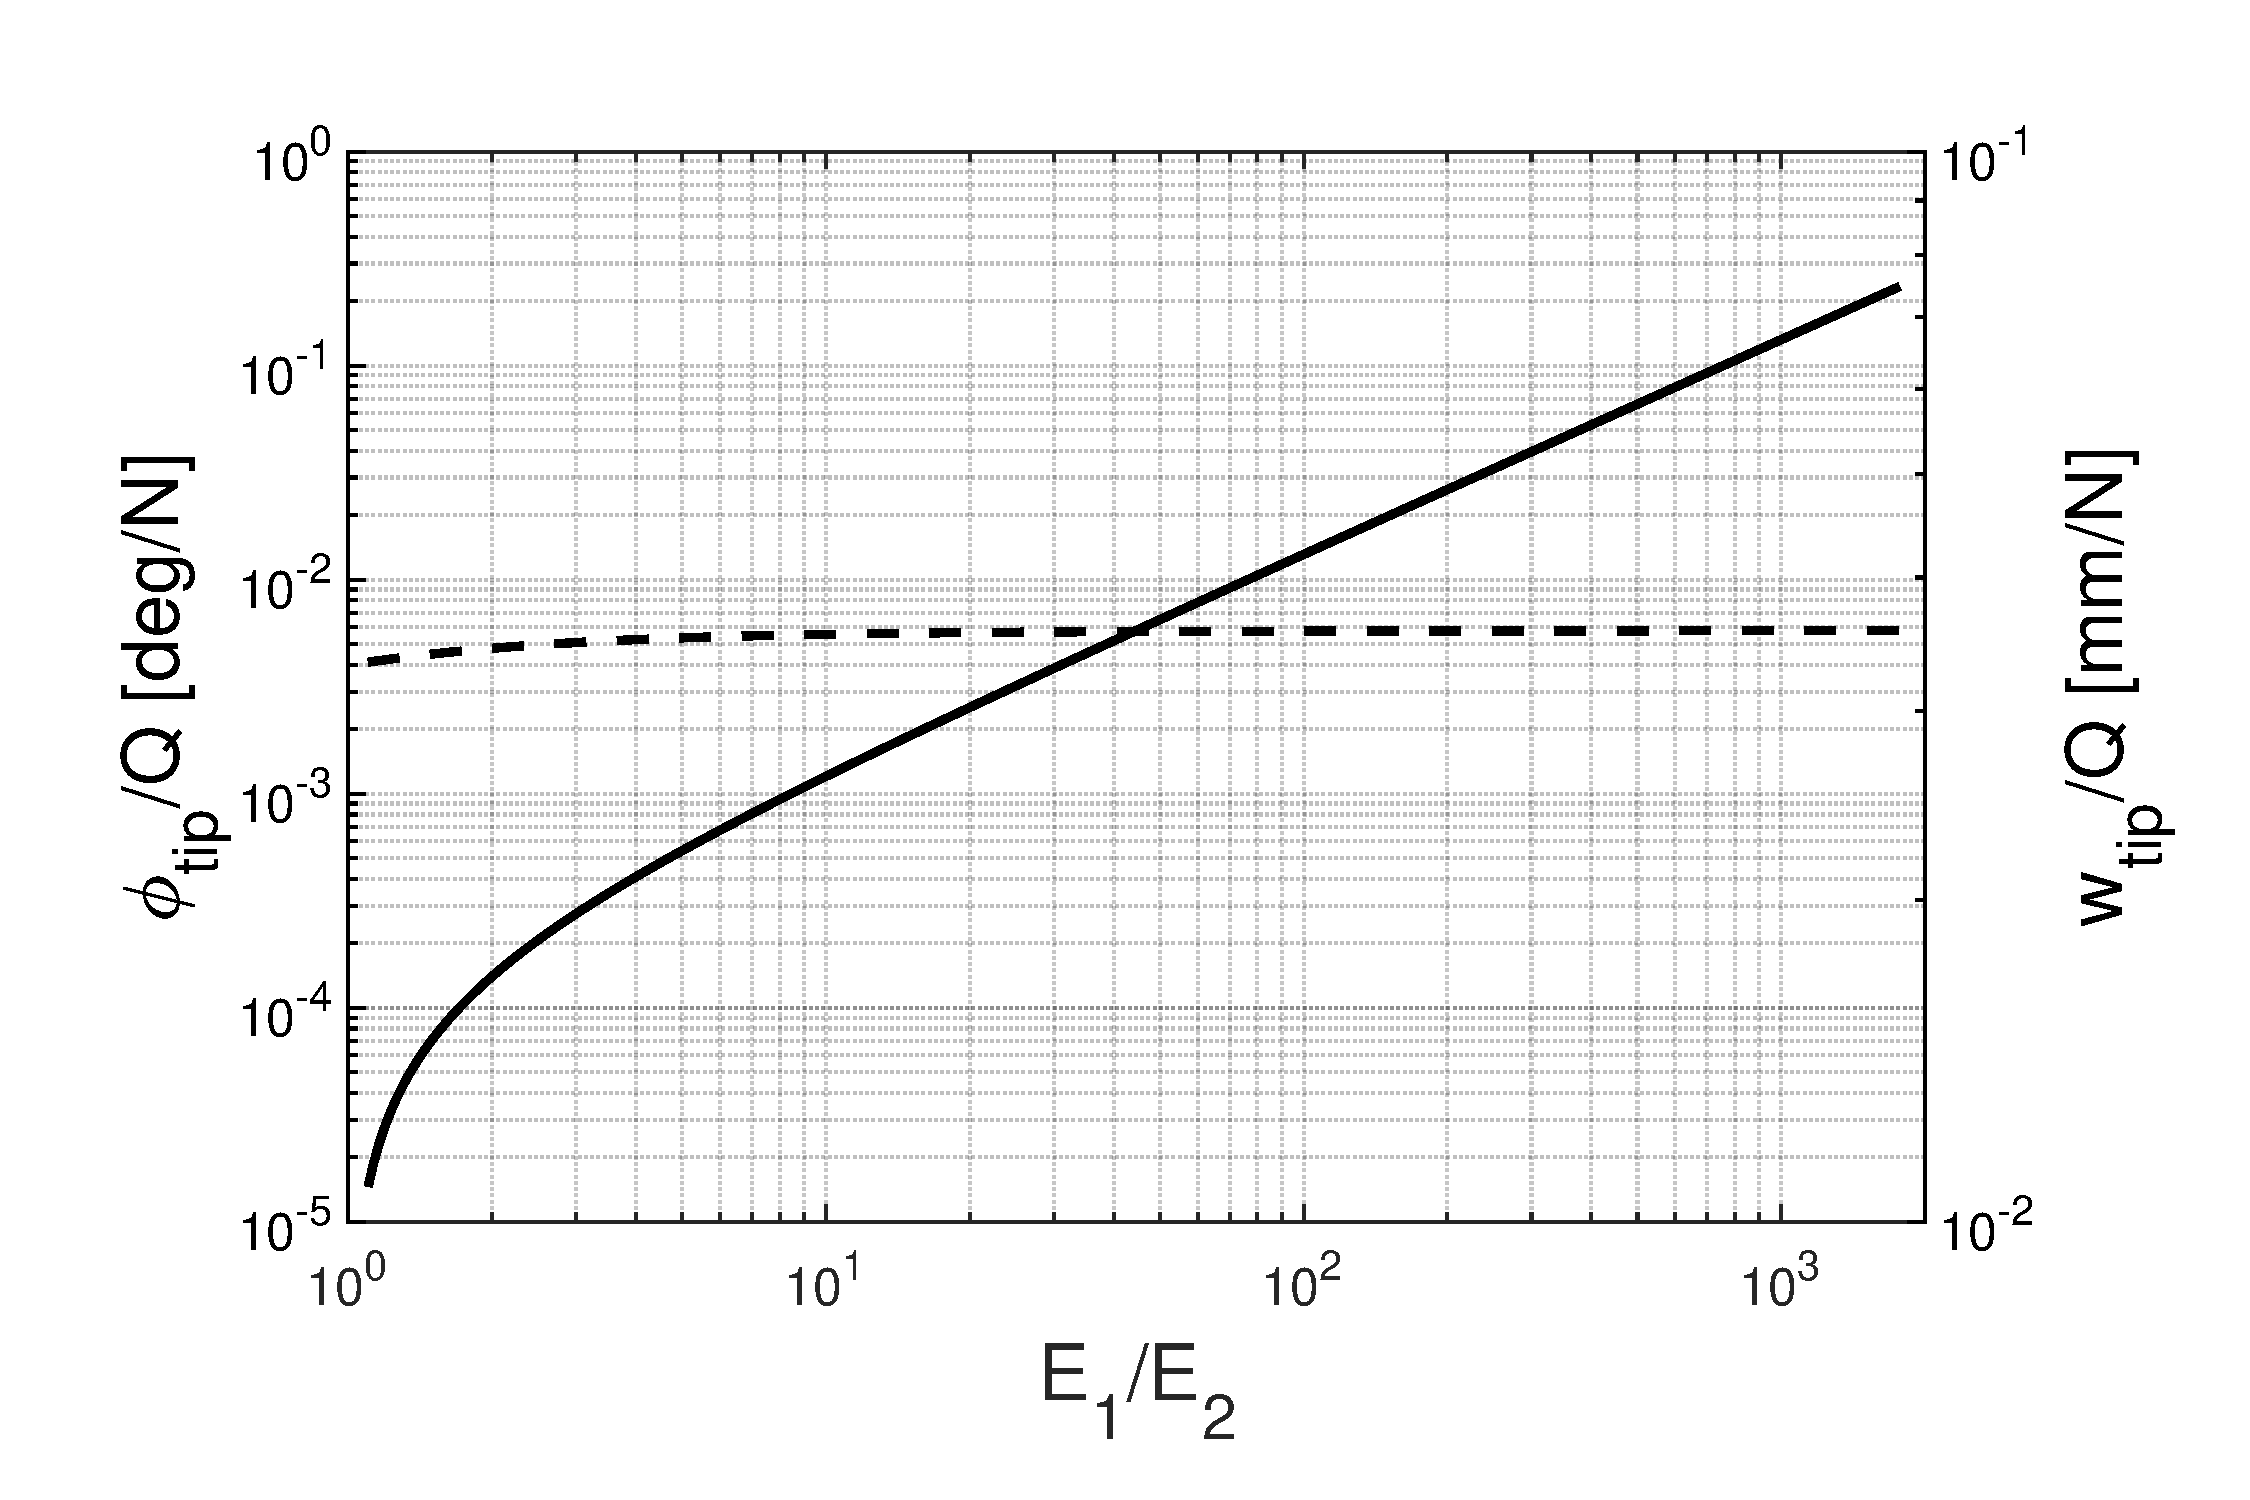
\includegraphics[width=0.8 \textwidth]{../analytical/figures/twist-E1overE2}
      \caption[Influence of the stiffness ratio on the wing-box tip twist and bend]{Influence of the stiffness ratio $E_1/E_2$ on the wing-box tip twist $\phi_{\mathrm{tip}}$ and bend $w_{\mathrm{tip}}$. The solid line is used to represent the twist $\phi_{\mathrm{tip}}$ while the dashed line represents the bend $w_{\mathrm{tip}}$. The two displacements correspond to values seen in the wing-box tip and are divided by the applied force magnitude $Q_z$.}\label{fig:twist-E1overE2}
    \end{figure}

    In Figure \ref{fig:twist-E1overE2}, the stiffness ratio $E_1/E_2$ is modified over a wide range such that $E_1/E_2 \in [10^{0}, 10^{3}]$. It can be seen that the variable $\phi_{\mathrm{tip}}/Q_z$ is consequently increased by various orders of magnitude from $\phi_{\mathrm{tip}}/Q_z = 10^{-4}$ deg/N to $\phi_{\mathrm{tip}}/Q_z = 10^{-1}$ deg/N, as a consequence of the stiffness ratio variation. However, the variation in bend represented with the variable $w_{\mathrm{tip}}/Q_z$ is negligible in comparison. It can be seen that the bending displacement quickly increases for values of $E_1/E_2 > 1$ and it gets to an asymptote for values $E_1/E_2 \gg 1$. These results therefore show how the twist displacement, which gives information regarding the torsional stiffness of the structure, is much more affected by variations of the stiffness ratio $E_1/E_2$ than the bending stiffness is. Consequently, it is not expected to see large increments in bend displacement in comparison with twist displacement when the variable-stiffness mechanism is activated. This results are in compliance with those presented in \cite{Raither2013a}.

    For the proposed mechanism, it is expected that the ratio $E_1/E_2$, which is linked to the effective shear modulus $G_{\mathrm{eff}}$ of the real wing-box, is reduced in various orders of magnitude once the buckling phenomena is triggered. After this event, the results above show that the reduction in bending stiffness of the wing-box will be negligible in comparison with the reduction in torsional stiffness.

  \subsection{Parametric study results and discussion} \label{subsec:results_parametricStudy}

    In the present subsection, the variation of the beam mechanical properties for different geometric parameter values is shown. The beam geometry is characterized through the cross-sectional aspect ratio $B/H$, the thickness ratio $t_2/t_1$ and the slenderness ratio $L/B$. The effect of these parameters on the sectional properties, twist and bending stiffness, and flexural and twisting compliance are shown. Additionally, the variance of the stiffness ratio $E_1/E_2$ is also included in the analysis.

    The influence of the cross-sectional aspect ratio $B/H$ on the torsional stiffness $G I_t$, the shear centre position $y_{\mathrm{SC}}$ and the flexural stiffness $E I_y$ is shown in Figures \ref{fig:GIt-E1overE2-BoverH}, \ref{fig:SC-E1overE2-BoverH} and \ref{fig:EIy-E1overE2-BoverH}, respectively. On its side, the effect of thickness ratio $t_2/t_1$ on the same three beam parameters is shown in Figures \ref{fig:GIt-E1overE2-t2overt1}, \ref{fig:SC-E1overE2-t2overt1} and \ref{fig:EIy-E1overE2-t2overt1}.

    %Figures variation of B/H
    \begin{figure}[!htpb] %G I_t versus B/H
      \centering
      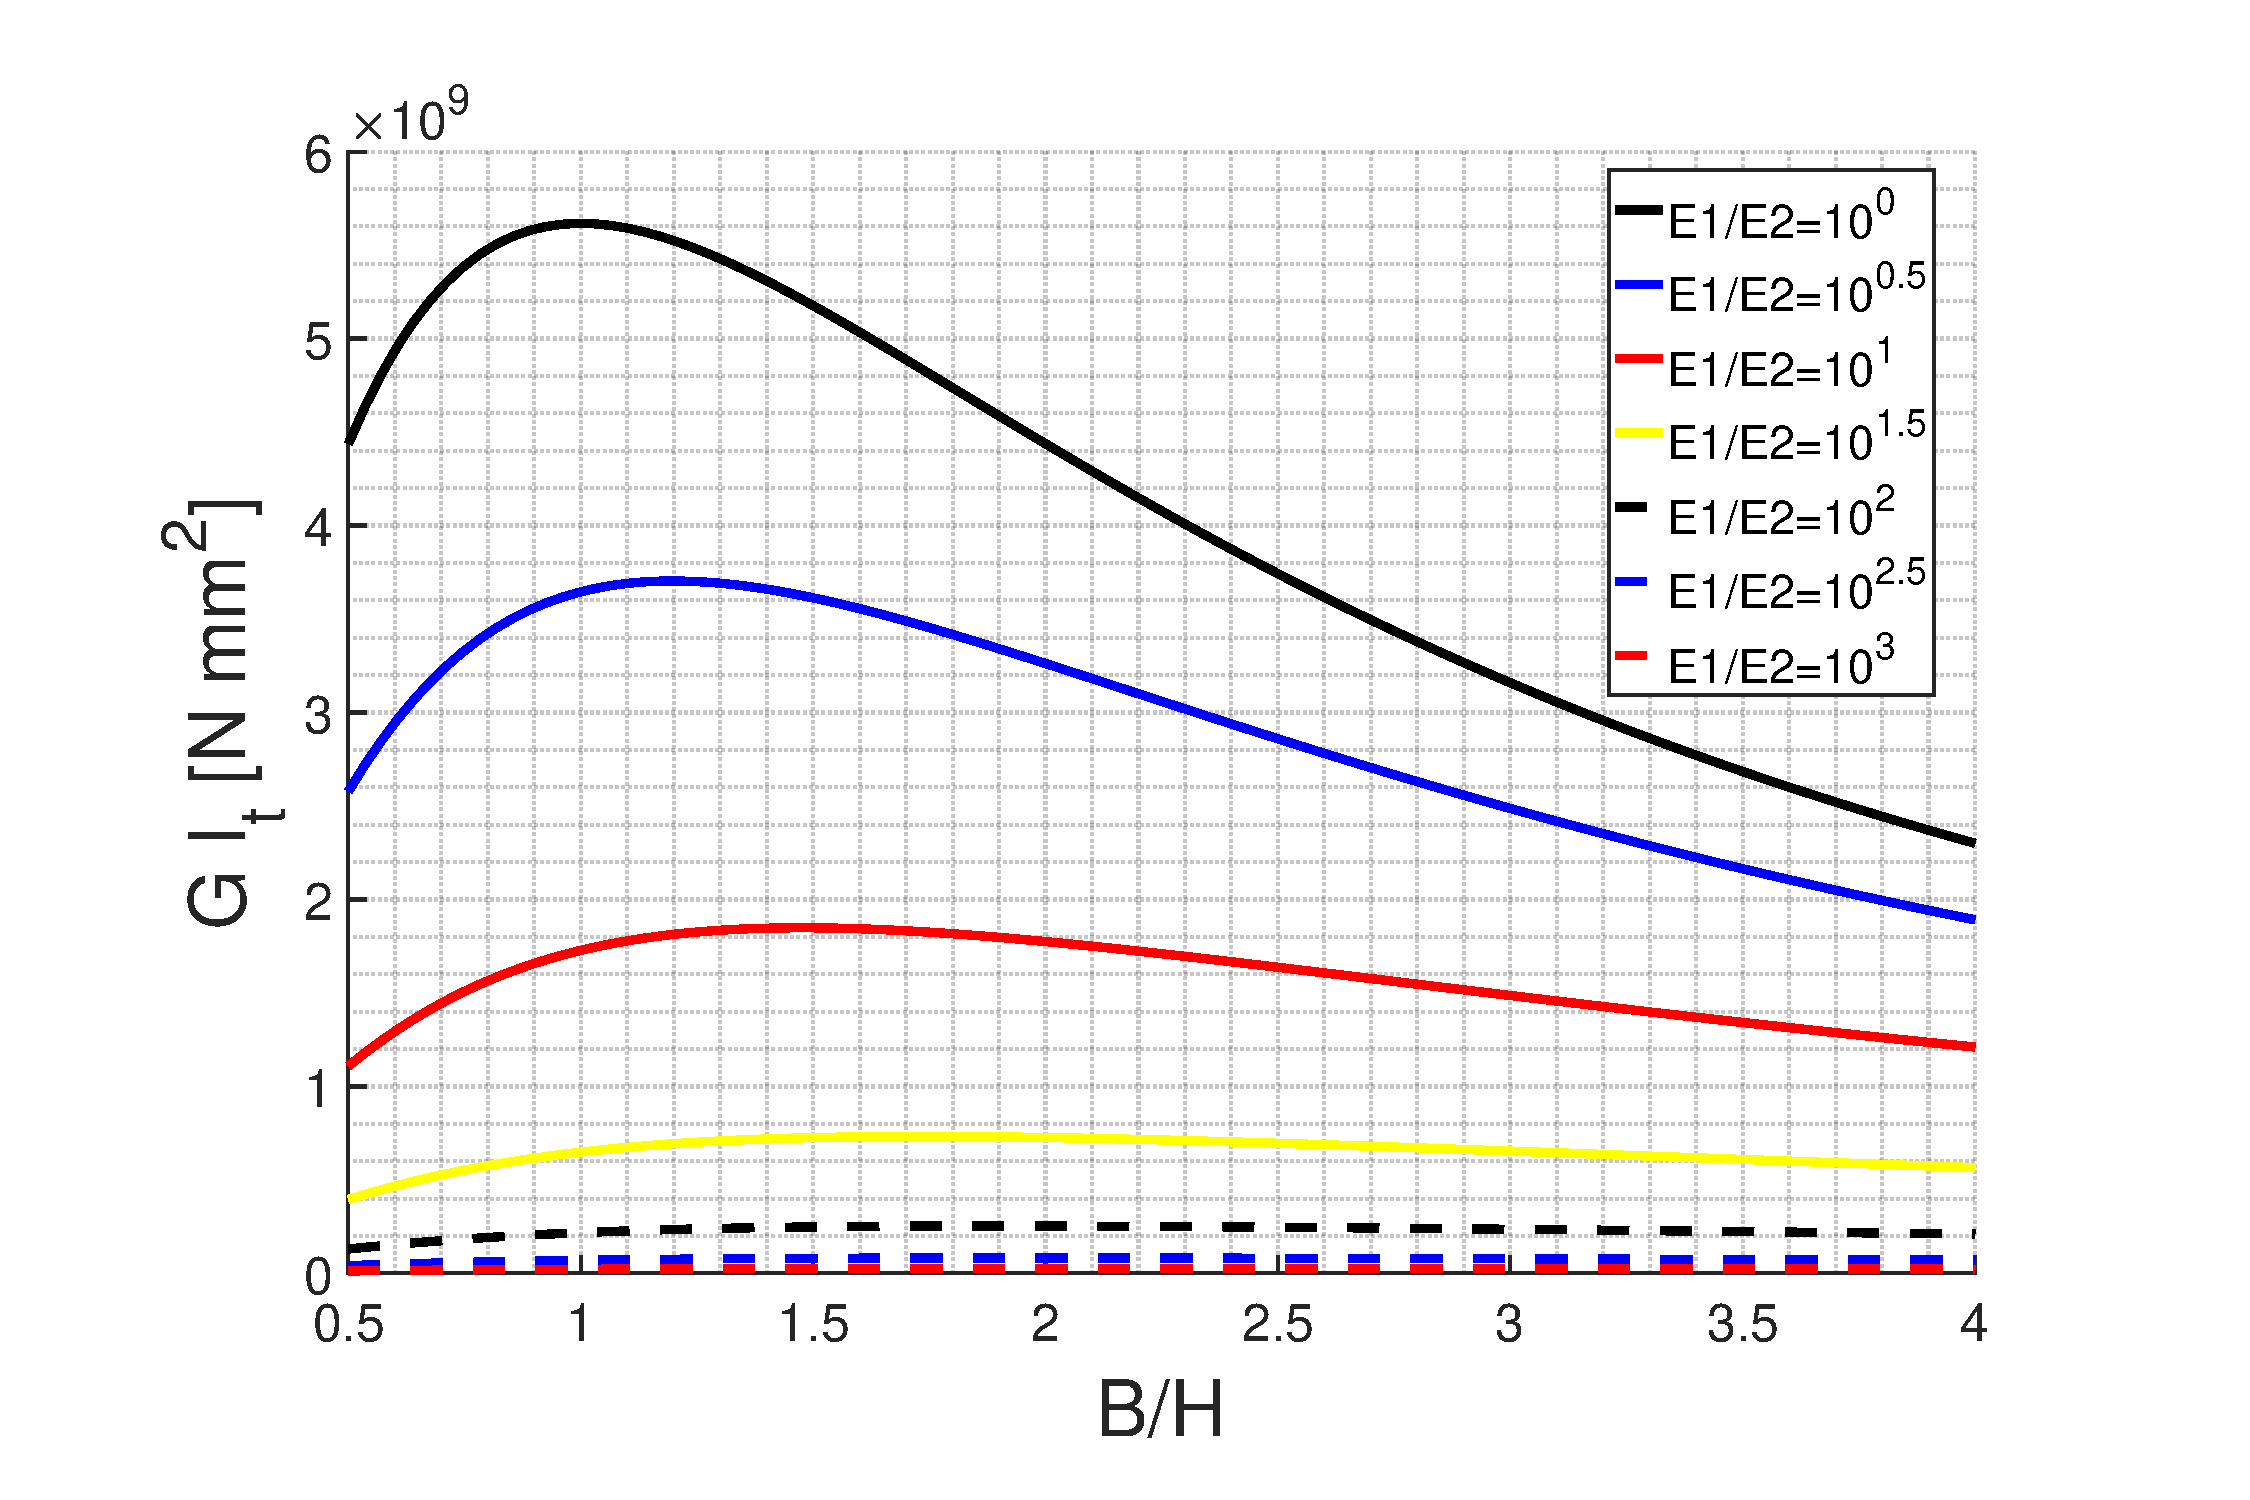
\includegraphics[width=0.8 \textwidth]{../analytical/figures/GIt-E1overE2-BoverH}
      \caption[Influence of the cross-sectional aspect ratio $B/H$ on the torsional stiffness $GI_t$]{Influence of the cross-sectional aspect ratio $B/H$ on the torsional stiffness $GI_t$, shown for various values of the stiffness ratio $E_1/E_2$ ranging from $10^0$ to $10^3$. }\label{fig:GIt-E1overE2-BoverH}
    \end{figure}

    \begin{figure}[!htpb] %Shear centre versus B/H
      \centering
      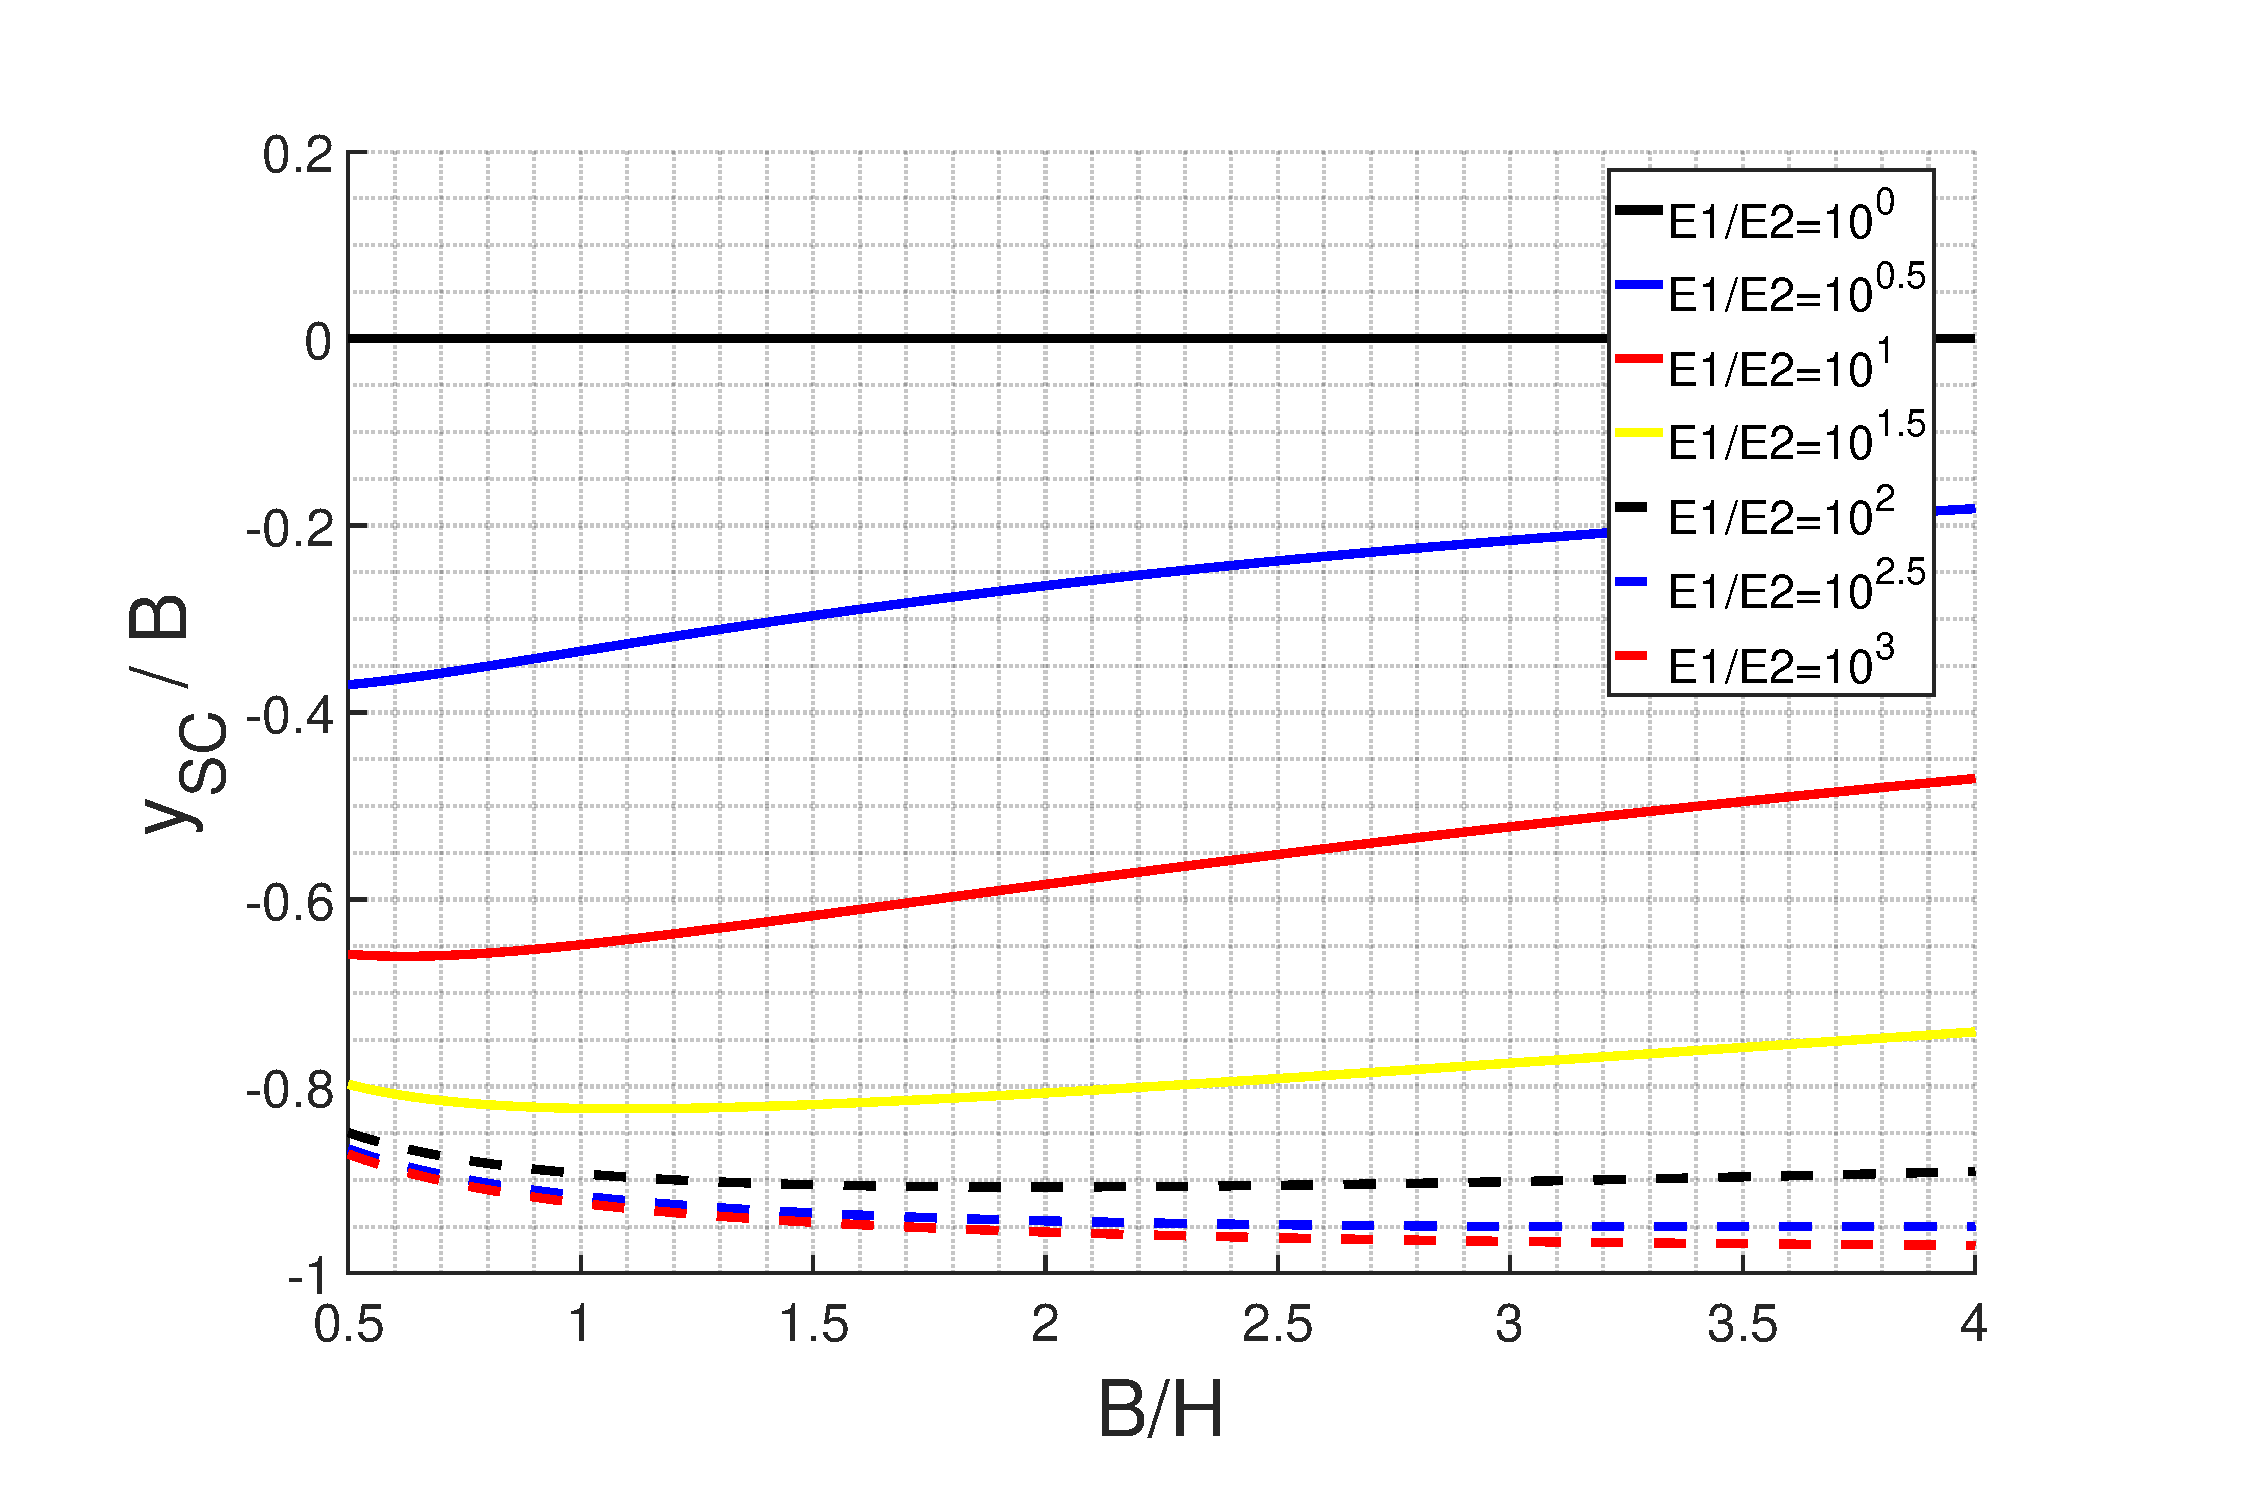
\includegraphics[width=0.8 \textwidth]{../analytical/figures/SC-E1overE2-BoverH}
      \caption[Influence of the cross-sectional aspect ratio $B/H$ on the dimensionless shear centre position $y_{\mathrm{SC}}/B$]{Influence of the cross-sectional aspect ratio $B/H$ on the dimensionless shear centre position $y_{\mathrm{SC}}/B$, shown for various values of the stiffness ratio $E_1/E_2$ ranging from $10^0$ to $10^3$. }\label{fig:SC-E1overE2-BoverH}
    \end{figure}

    \begin{figure}[!htpb] %E I_y = \Phi_y versus B/H
      \centering
      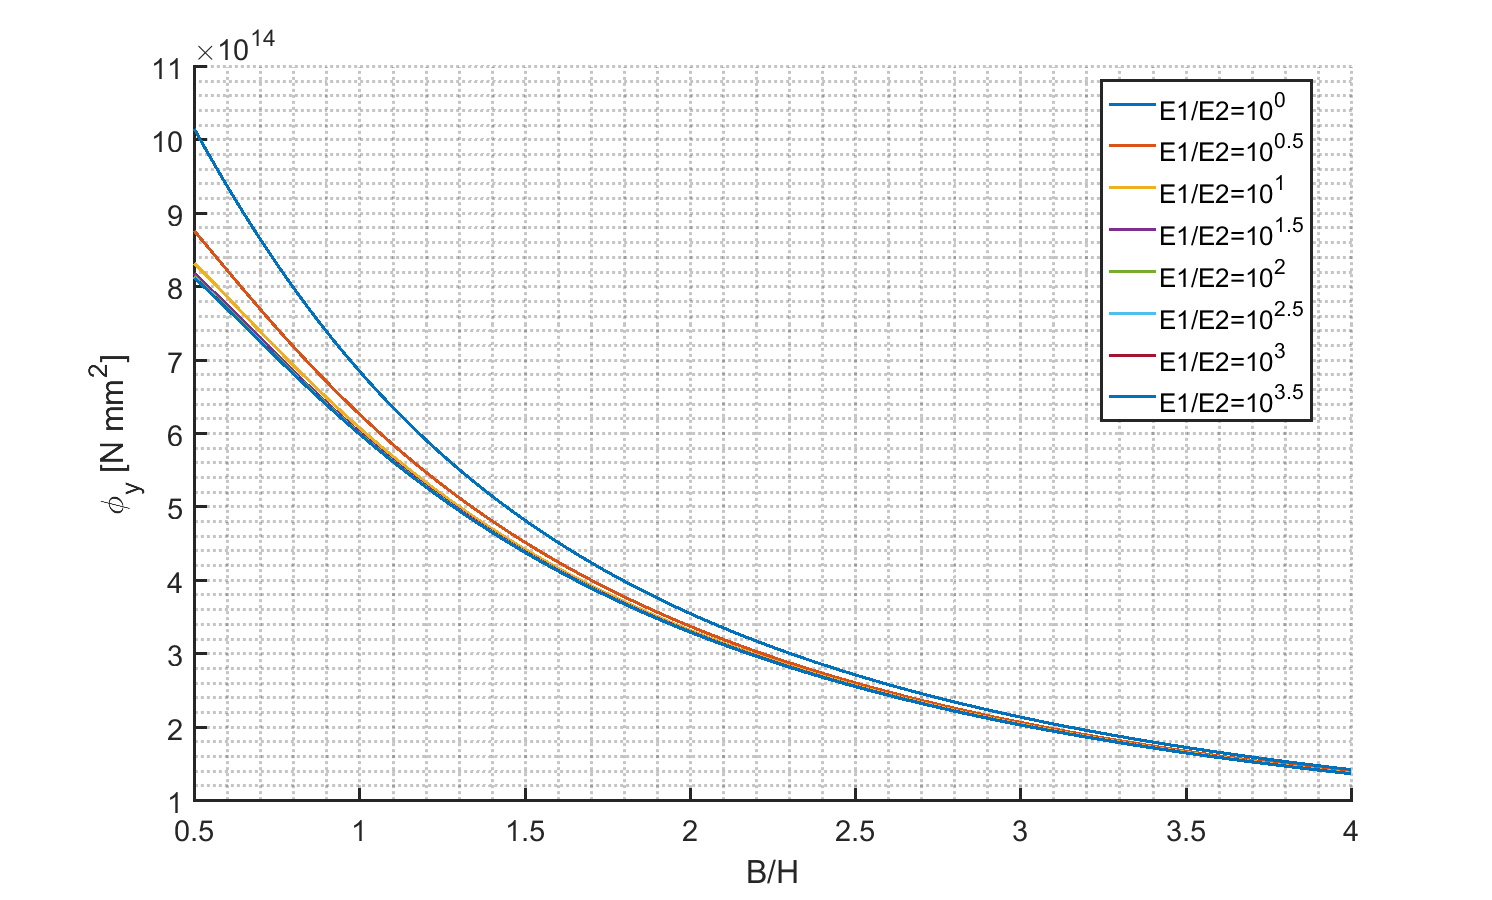
\includegraphics[width=0.8 \textwidth]{../analytical/figures/EIy-E1overE2-BoverH}
      \caption[Influence of the cross-sectional aspect ratio $B/H$ on the flexural stiffness $EI_y$]{Influence of the cross-sectional aspect ratio $B/H$ on the flexural stiffness $EI_y = \Phi_y$, shown for various values of the stiffness ratio $E_1/E_2$ ranging from $10^0$ to $10^3$. }\label{fig:EIy-E1overE2-BoverH}
    \end{figure}

    %%%% Figures variation of t2/t1
    \begin{figure}[!htpb] %G I_t versus t2/t1
      \centering
      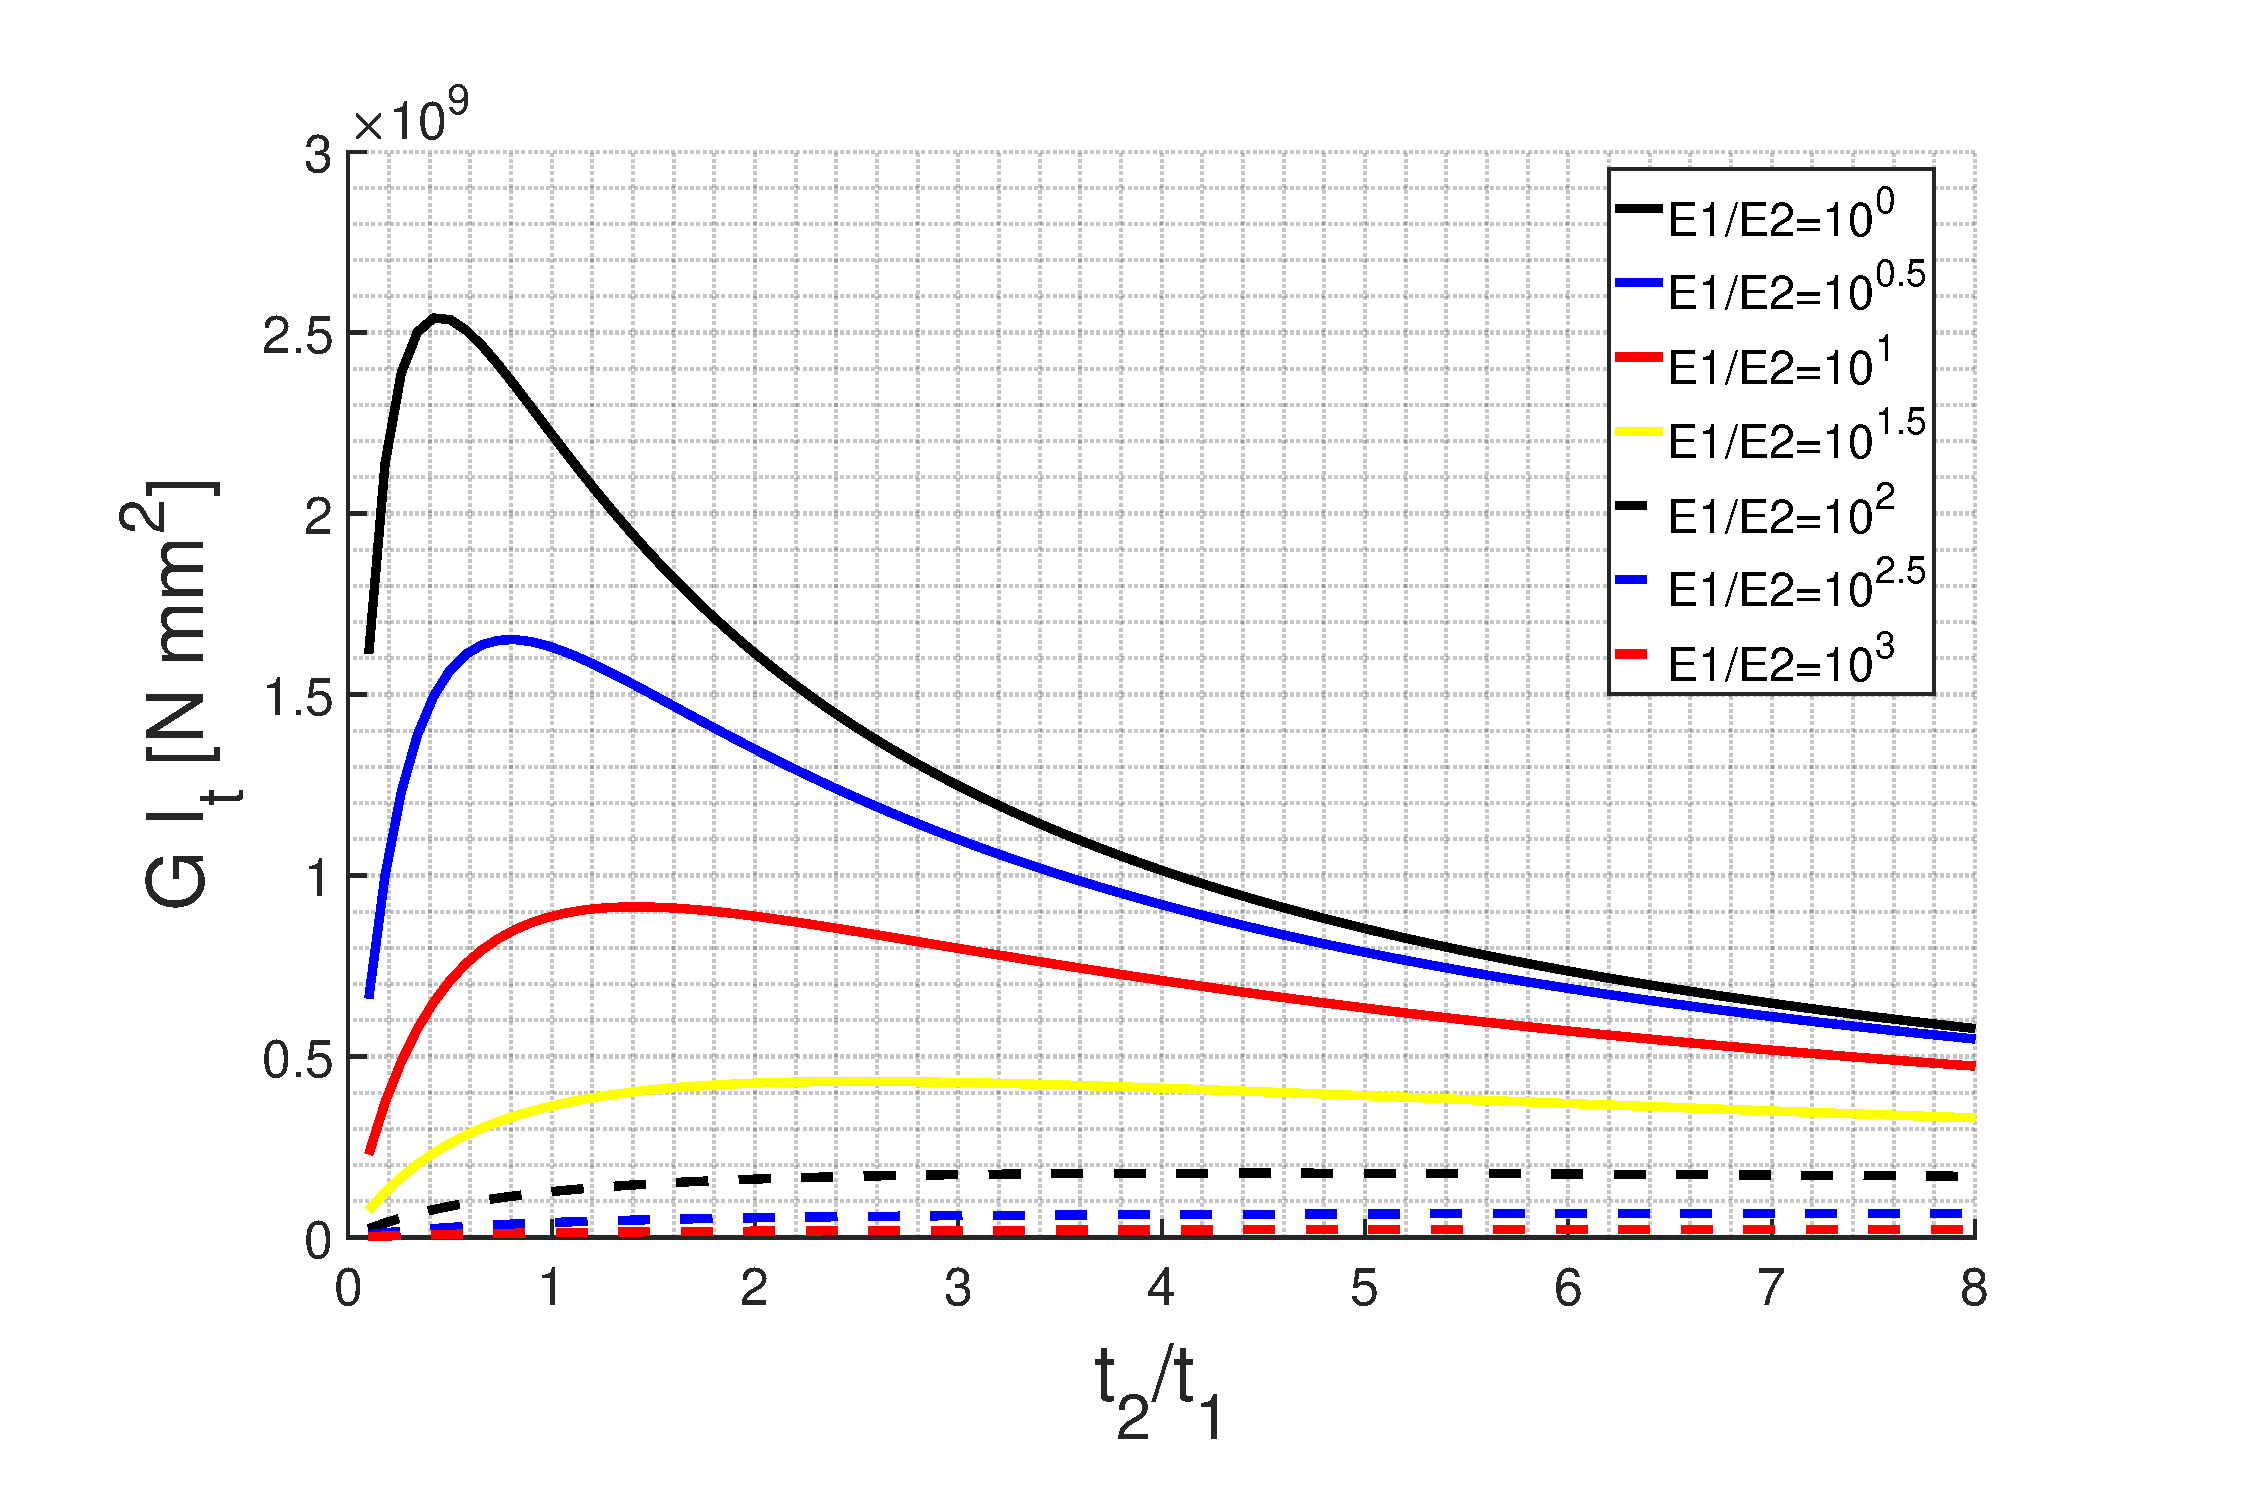
\includegraphics[width=0.8 \textwidth]{../analytical/figures/GIt-E1overE2-t2overt1}
      \caption[Influence of the wall thickness ratio $t_2/t_1$ on the torsional stiffness $GI_t$]{Influence of the wall thickness ratio $t_2/t_1$ on the torsional stiffness $GI_t$, shown for various values of the stiffness ratio $E_1/E_2$ ranging from $10^0$ to $10^3$. }\label{fig:GIt-E1overE2-t2overt1}
    \end{figure}

    \begin{figure}[!htpb] %Shear centre versus t2/t1
      \centering
      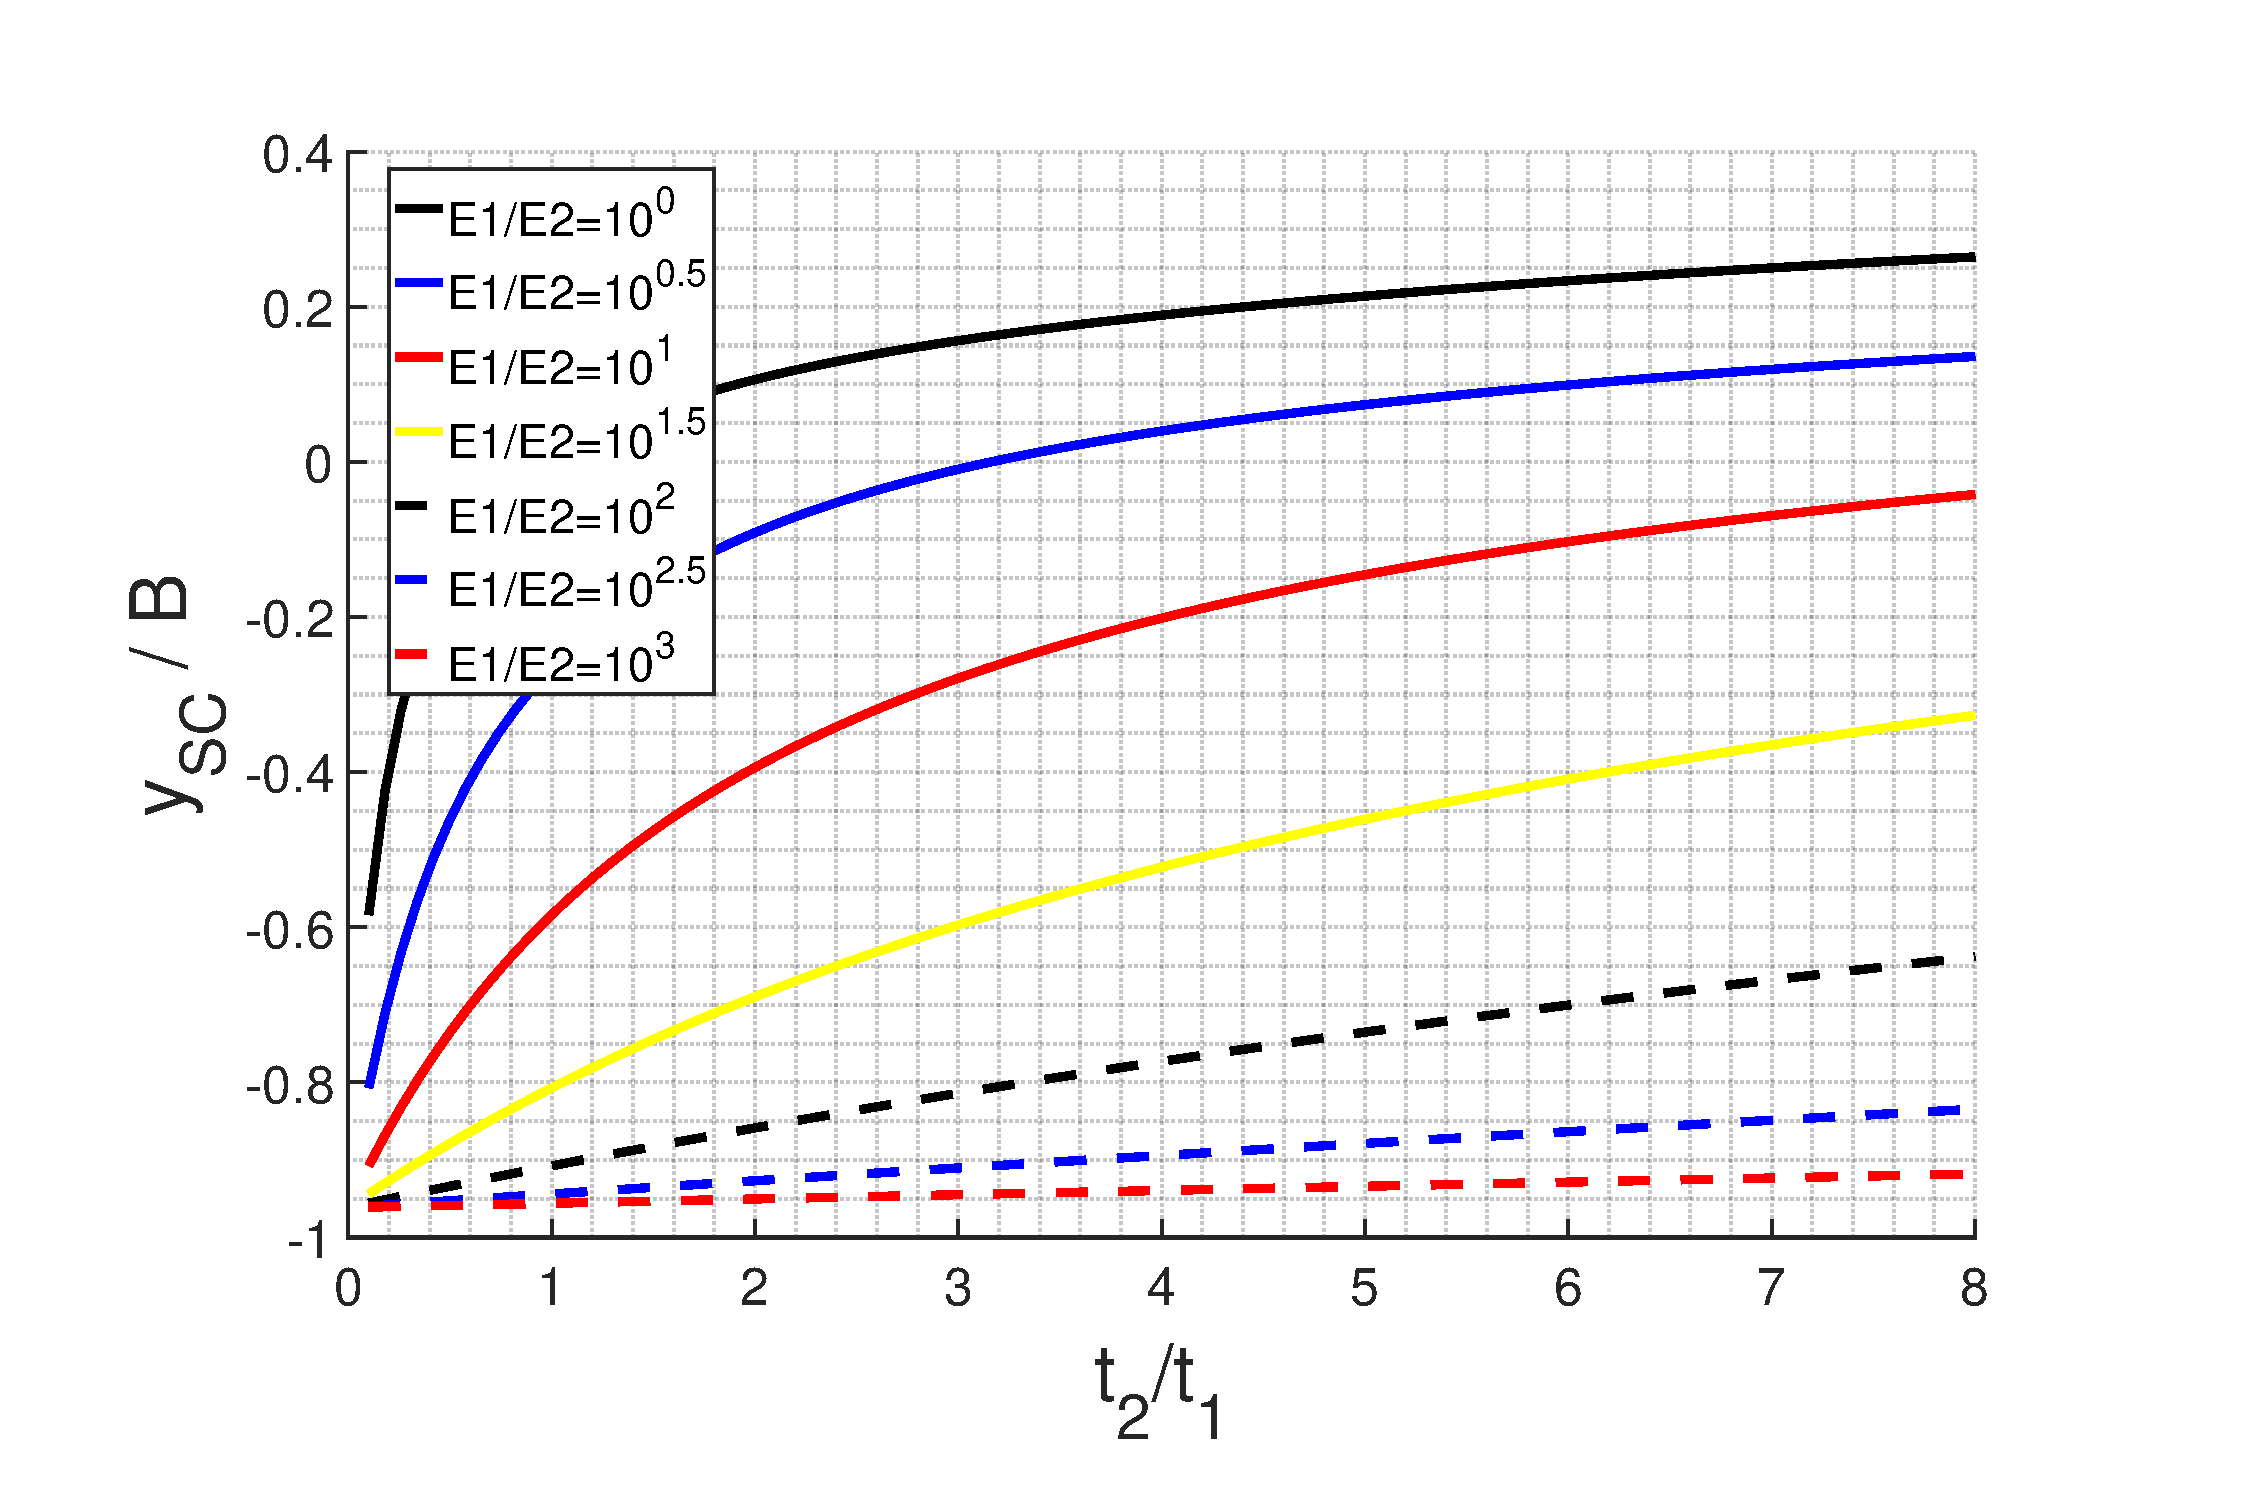
\includegraphics[width=0.8 \textwidth]{../analytical/figures/SC-E1overE2-t2overt1}
      \caption[Influence of the wall thickness ratio $t_2/t_1$ on the dimensionless shear centre position $y_{\mathrm{SC}}/B$]{Influence of the wall thickness ratio $t_2/t_1$ on the dimensionless shear centre position $y_{\mathrm{SC}}/B$, shown for various values of the stiffness ratio $E_1/E_2$ ranging from $10^0$ to $10^3$. }\label{fig:SC-E1overE2-t2overt1}
    \end{figure}

    \begin{figure}[!htpb] %E I_y = \Phi_y versus t2/t1
      \centering
      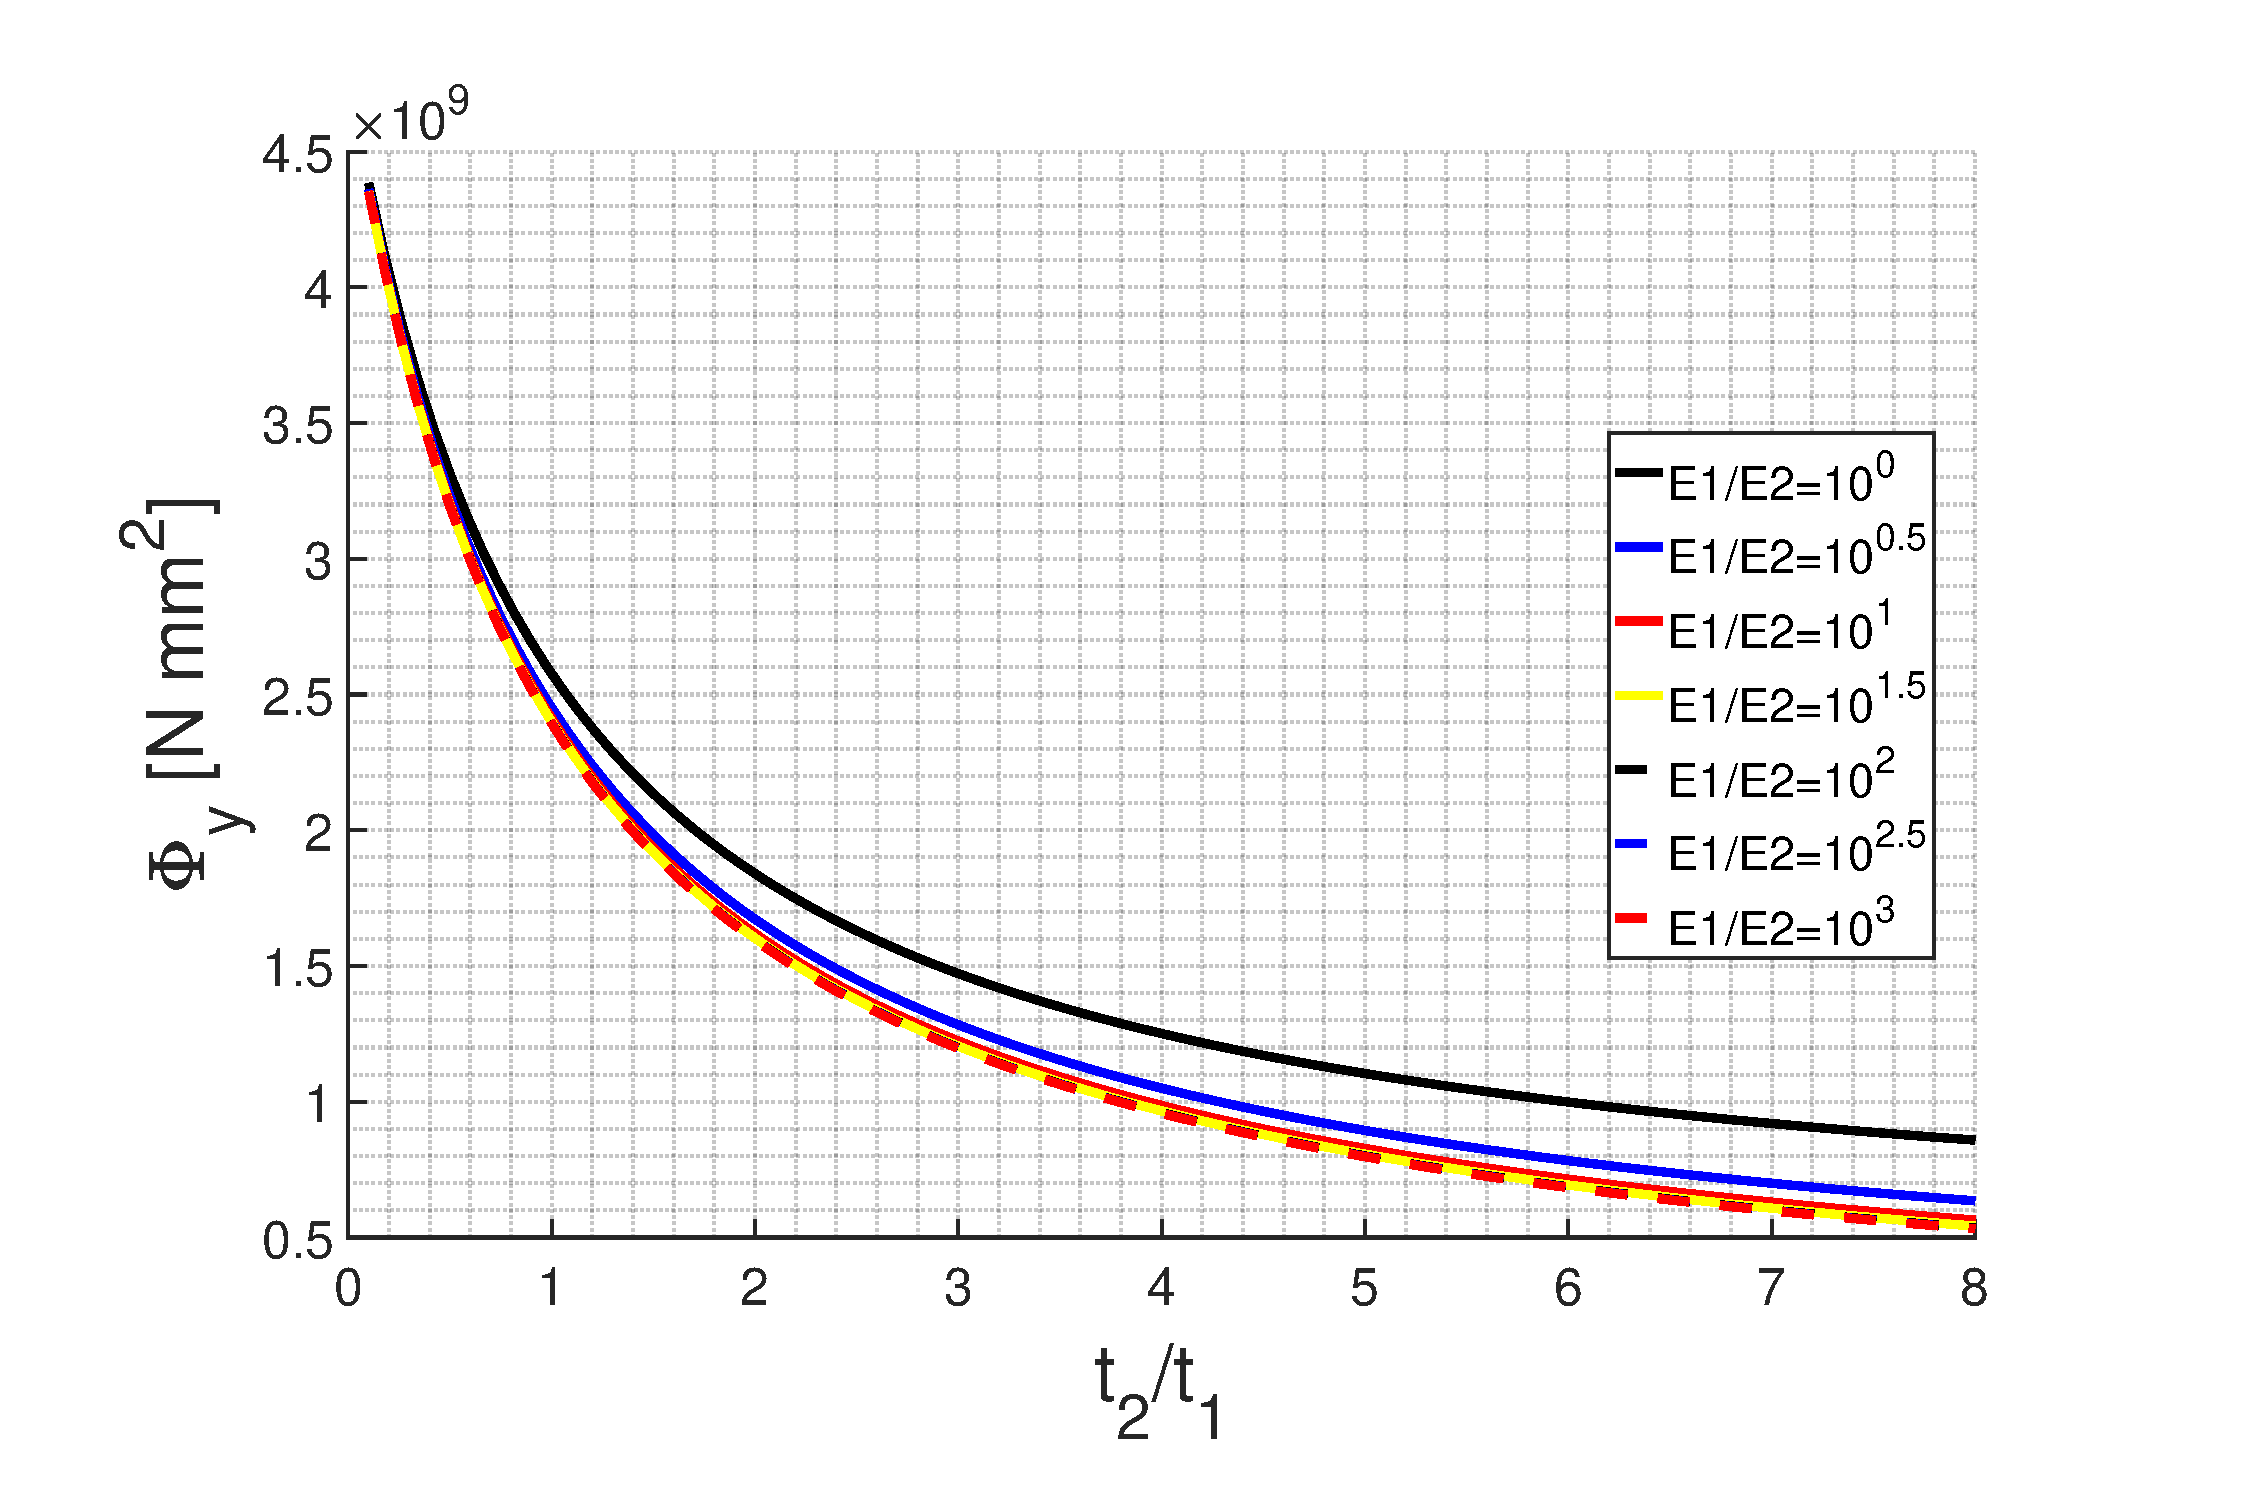
\includegraphics[width=0.8 \textwidth]{../analytical/figures/EIy-E1overE2-t2overt1}
      \caption[Influence of the wall thickness ratio $t_2/t_1$ on the flexural stiffness $EI_y$]{Influence of the wall thickness ratio $t_2/t_1$ on the flexural stiffness $EI_y = \Phi_y$, shown for various values of the stiffness ratio $E_1/E_2$ ranging from $10^0$ to $10^3$. }\label{fig:EIy-E1overE2-t2overt1}
    \end{figure}

    \clearpage
    In Figure \ref{fig:GIt-E1overE2-BoverH}, it can be seen that a maximum torsional stiffness appears for $B/H = 1$ when $E_1/E_2 = 1$. This can be explained because, as it is also shown in \cite{Raither2013a}, the closer the torsional stiffness to the doubly symmetric case, the higher its torsional stiffness. However, when $E_1/E_2 > 10$, the maximum torsional stiffness is shown to appear for $B/H > 1$. A similar conclusion can be extract when analyzing the Figure \ref{fig:GIt-E1overE2-t2overt1}, that shows the influence of the thickness ratio $t_2/t_1$ on the torsional stiffness $G I_t$.

    In Figure \ref{fig:SC-E1overE2-BoverH} shows that for values $E_2 \ll E_1$, the shear centre position $y_{\mathrm{SC}}$ is approximately constant for $B/H$ variations. In this context, the beam approximates its behavior as if it has an open profile section. However, as the value of $E_1/E_2$ decreases, the influence of the ratio $B/H$ increases showing a bigger influence of the web where the Young's modulus $E_2$ applies. On the other hand, Figure \ref{fig:SC-E1overE2-t2overt1} shows that the bigger the thickness ratio $t_2/t_1$ is, the closer that the shear centre $y_{\mathrm{SC}}$ will be to the vertical axis of symmetry. However, for $E_2 \ll E_1$ the influence of the thickness ratio $t_2/t_1$ is reduced.

    In Figure \ref{fig:EIy-E1overE2-BoverH} it can be seen that the flexural stiffness $E I_y$ decreases when the cross-sectional aspect ratio $B/H$ increases. This is explained because the second moment of area $I_y$ is reduced when $B/H$ increases as the coordinate $y$ of the points in the section is reduced as well. Similarly, it can be seen in Figure \ref{fig:EIy-E1overE2-t2overt1} that when the thickness ratio $t_2/t_1$ increases, the value of $E I_y$ decreases. In both cases, the flexural stiffness $E I_y$ is little affected by variations of the stiffness ratio $E_1/E_2$. This result matches what was already shown in Subsection \ref{subsec:bendingTwistCoupling_results_model}.

    % Effect on deflection and torsional compliance
    Additionally, the effect of the cross-sectional aspect ratio $B/H$ on the deflection and torsional compliances is shown in Figures \ref{fig:woverQ-E1overE2-BoverH} and \ref{fig:phioverQ-E1overE2-BoverH}, respectively. The corresponding plots when analyzing the effect of the thickness ratio $t_2/t_1$ on the deflection and torsional compliance are shown on Figures \ref{fig:woverQ-E1overE2-t2overt1} and \ref{fig:phioverQ-E1overE2-t2overt1}, respectively. The beam torsional compliance is expressed as a fraction of the twist at the tip divided by the vertical force applied, that is $|\phi_{\mathrm{tip}}| / Q$, while the beam flexural compliance is expressed as fraction of the maximum vertical displacement at the tip divided by the vertical force applied, that is $w_{\mathrm{0,tip}} / Q$.

    % Displacements
    \begin{figure}[!htpb] %w_0,tip / Q versus B/H, flexural compliance
      \centering
      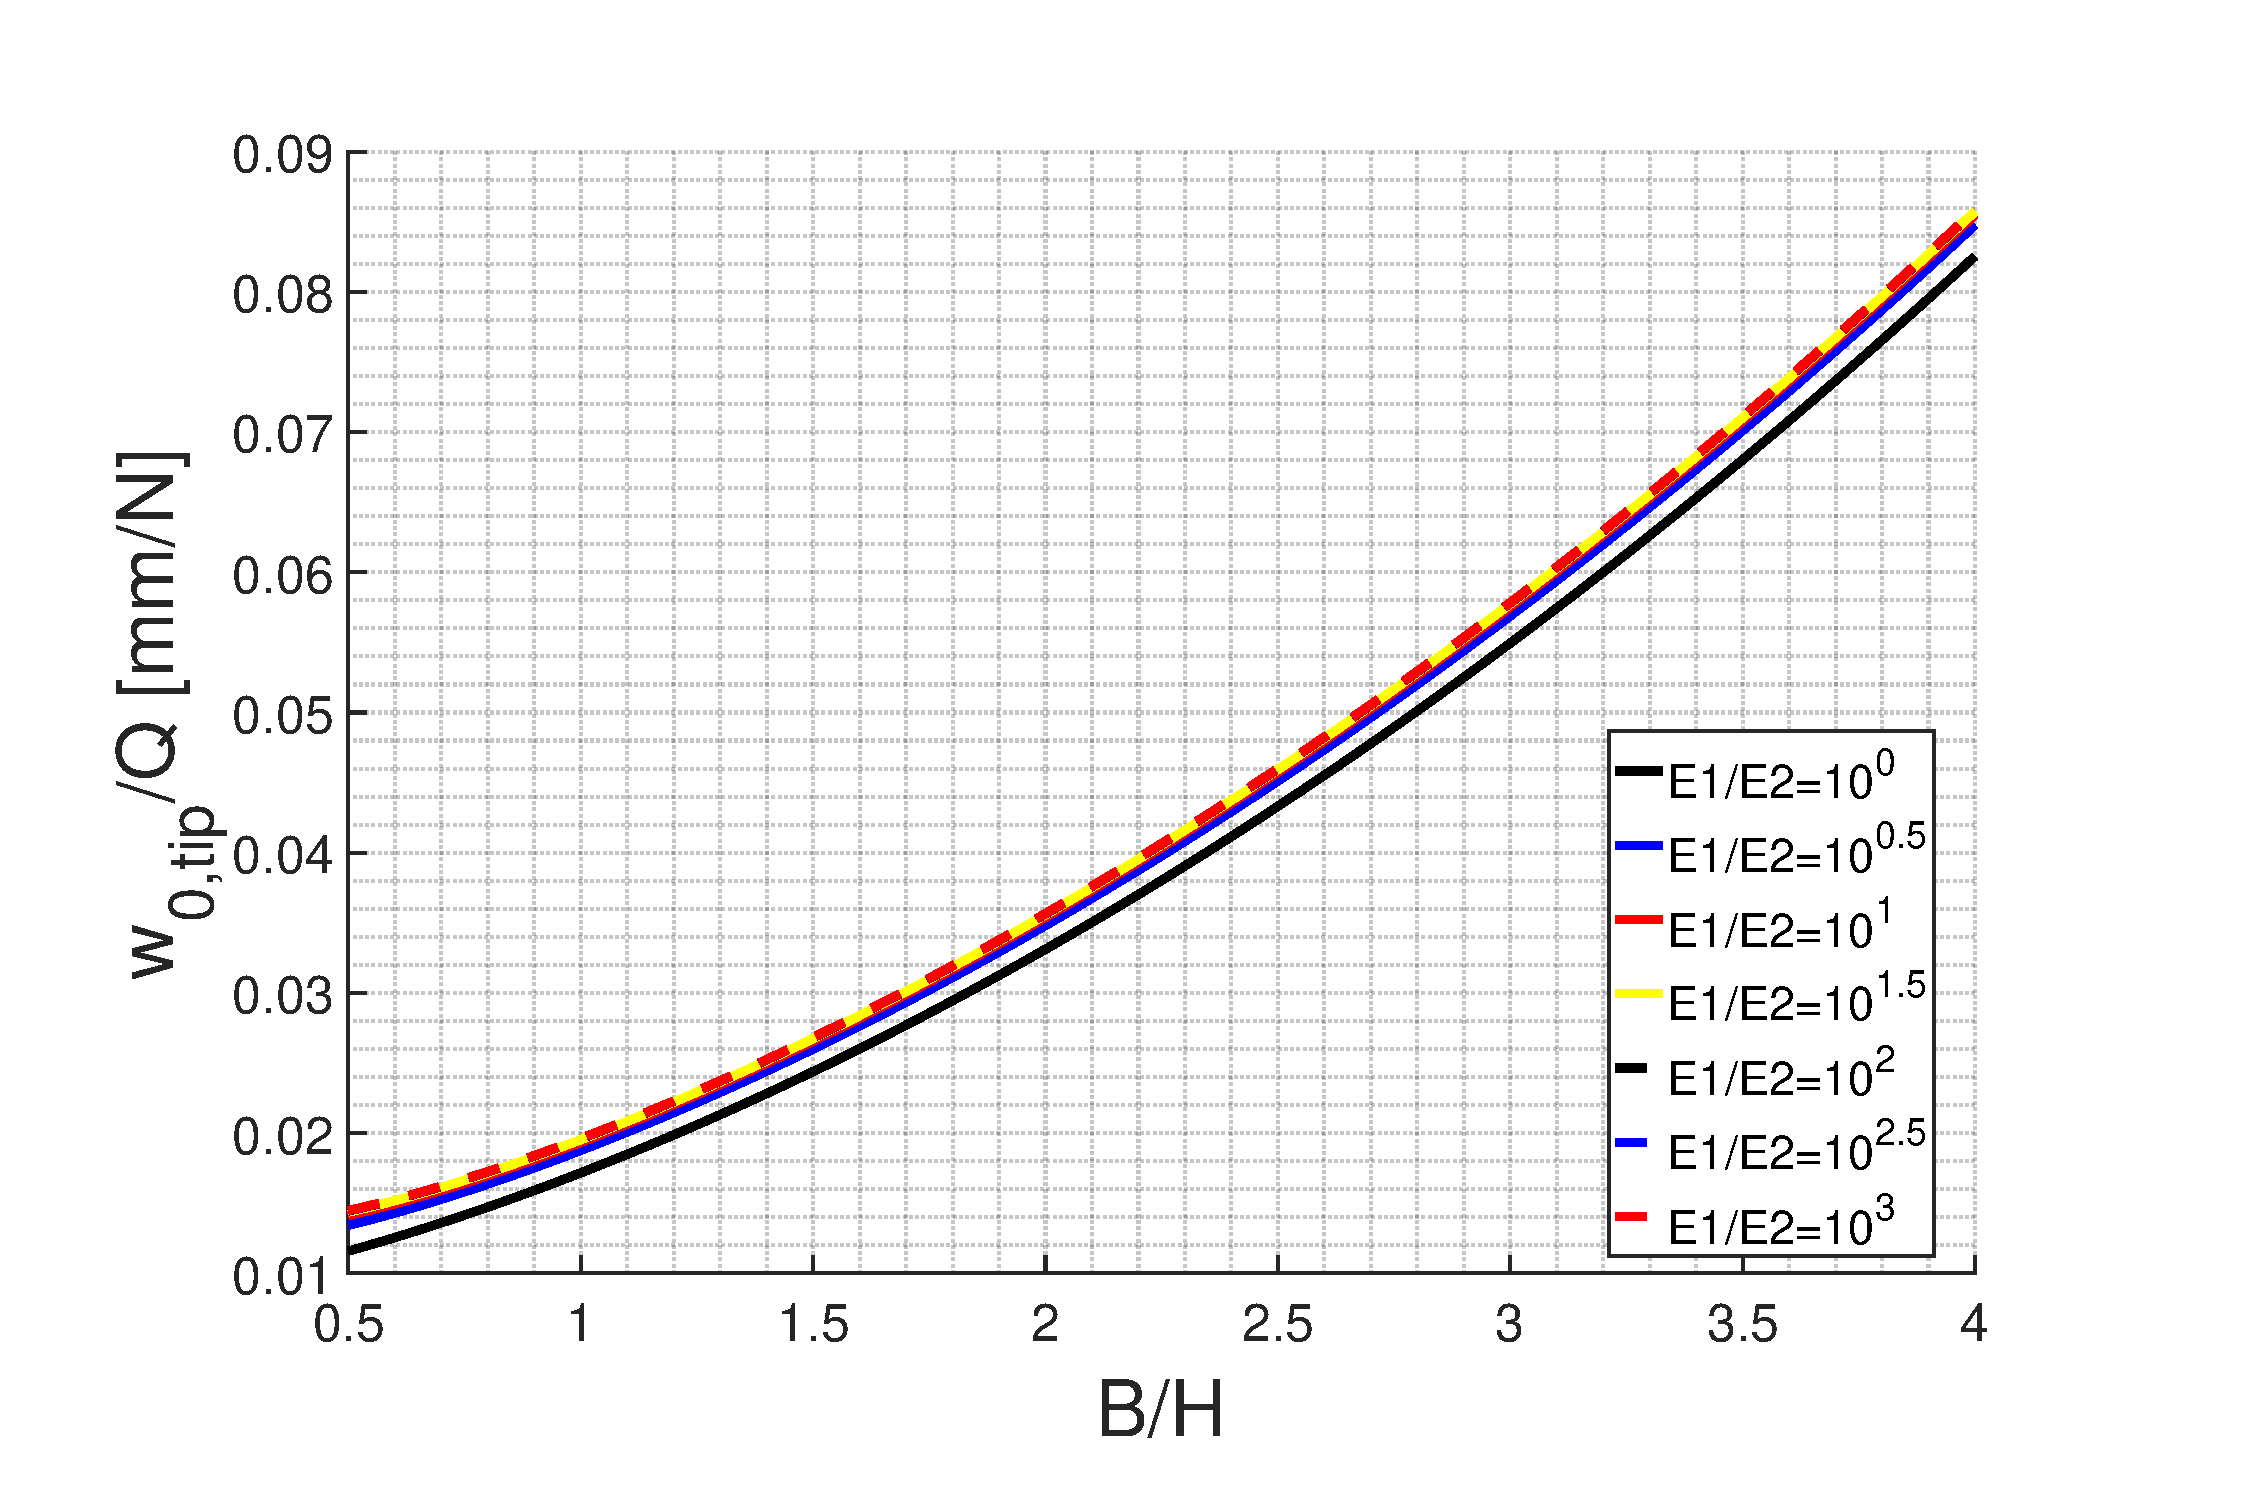
\includegraphics[width=0.8 \textwidth]{../analytical/figures/woverQ-E1overE2-BoverH}
      \caption[Influence of the cross-sectional aspect ratio $B/H$ on the flexural compliance]{Influence of the cross-sectional aspect ratio $B/H$ on the flexural compliance $w_{\mathrm{0,tip}} / Q$, shown for various values of the stiffness ratio $E_1/E_2$ ranging from $10^0$ to $10^3$. }\label{fig:woverQ-E1overE2-BoverH}
    \end{figure}

    \begin{figure}[!htpb] %\phi_tip / Q versus B/H, torsional compliance
      \centering
      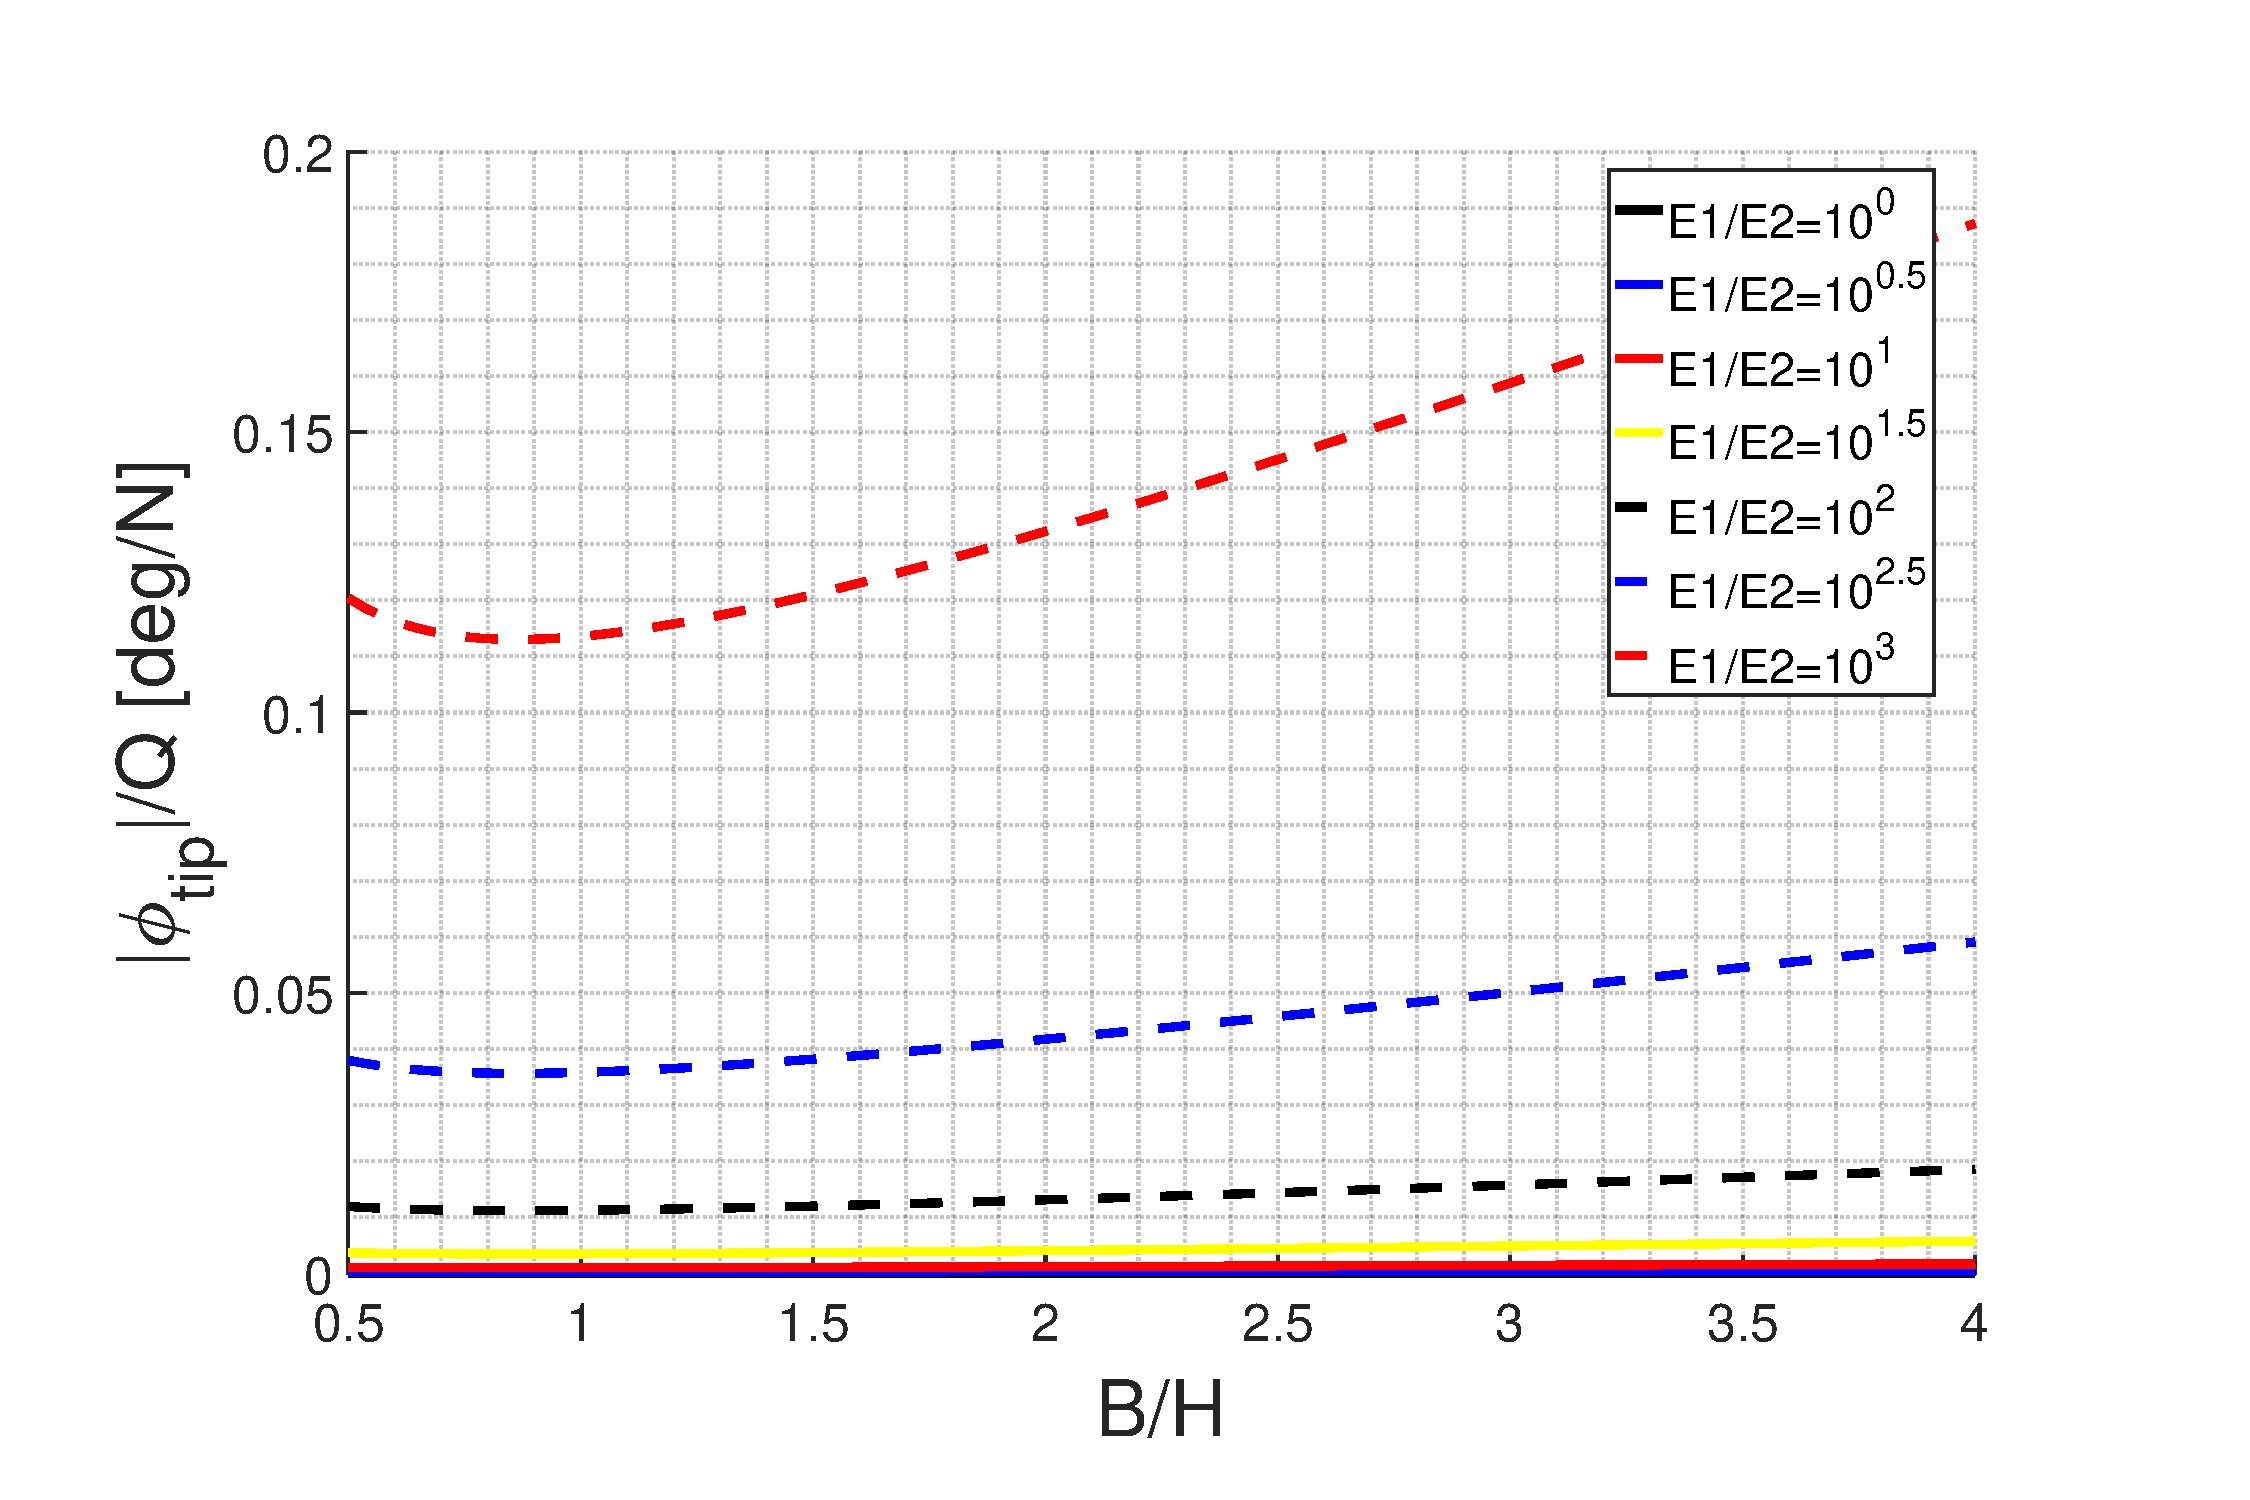
\includegraphics[width=0.8 \textwidth]{../analytical/figures/phioverQ-E1overE2-BoverH}
      \caption[Influence of the cross-sectional aspect ratio $B/H$ on the torsional compliance]{Influence of the cross-sectional aspect ratio $B/H$ on the torsional compliance $|\phi_{\mathrm{tip}}| / Q$, shown for various values of the stiffness ratio $E_1/E_2$ ranging from $10^0$ to $10^3$. }\label{fig:phioverQ-E1overE2-BoverH}
    \end{figure}

    \begin{figure}[!htpb] %w_0,tip / Q versus t2/t1, flexural compliance
      \centering
      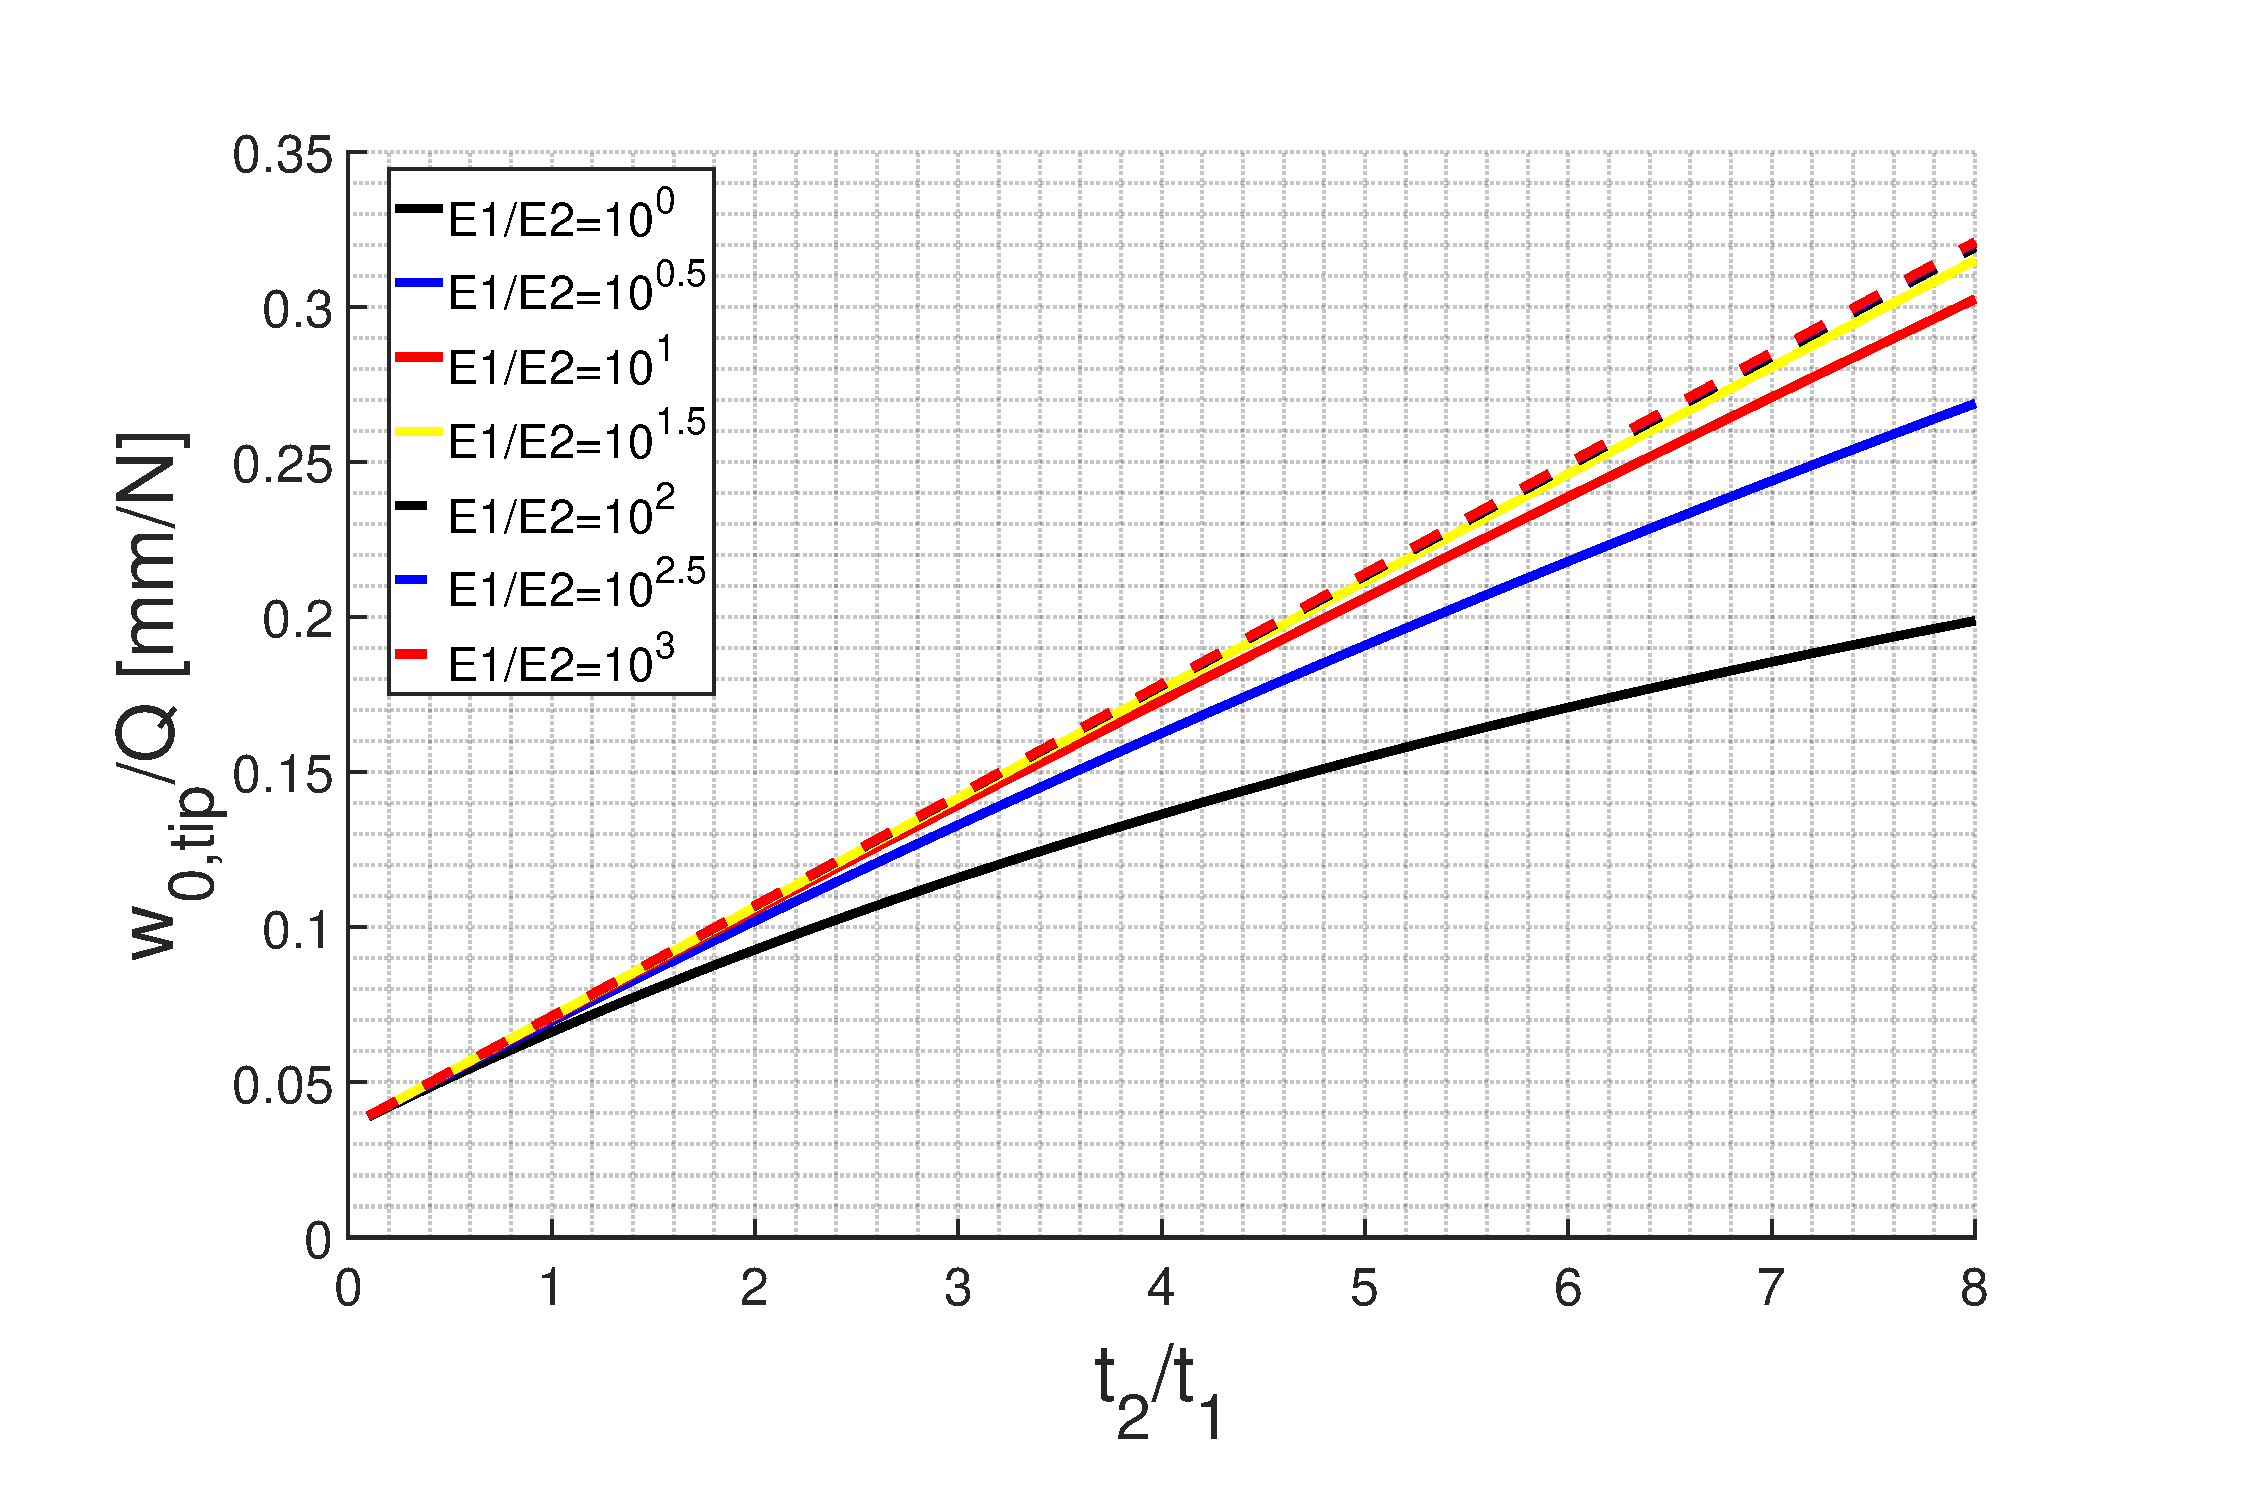
\includegraphics[width=0.8 \textwidth]{../analytical/figures/woverQ-E1overE2-t2overt1}
      \caption[Influence of the thickness ratio $t2/t1$ on the flexural compliance]{Influence of the thickness ratio $t2/t1$ on the flexural compliance $w_{\mathrm{0,tip}} / Q$, shown for various values of the stiffness ratio $E_1/E_2$ ranging from $10^0$ to $10^3$. }\label{fig:woverQ-E1overE2-t2overt1}
    \end{figure}

    \begin{figure}[!htpb] %\phi_tip / Q versus t2/t1, torsional compliance
      \centering
      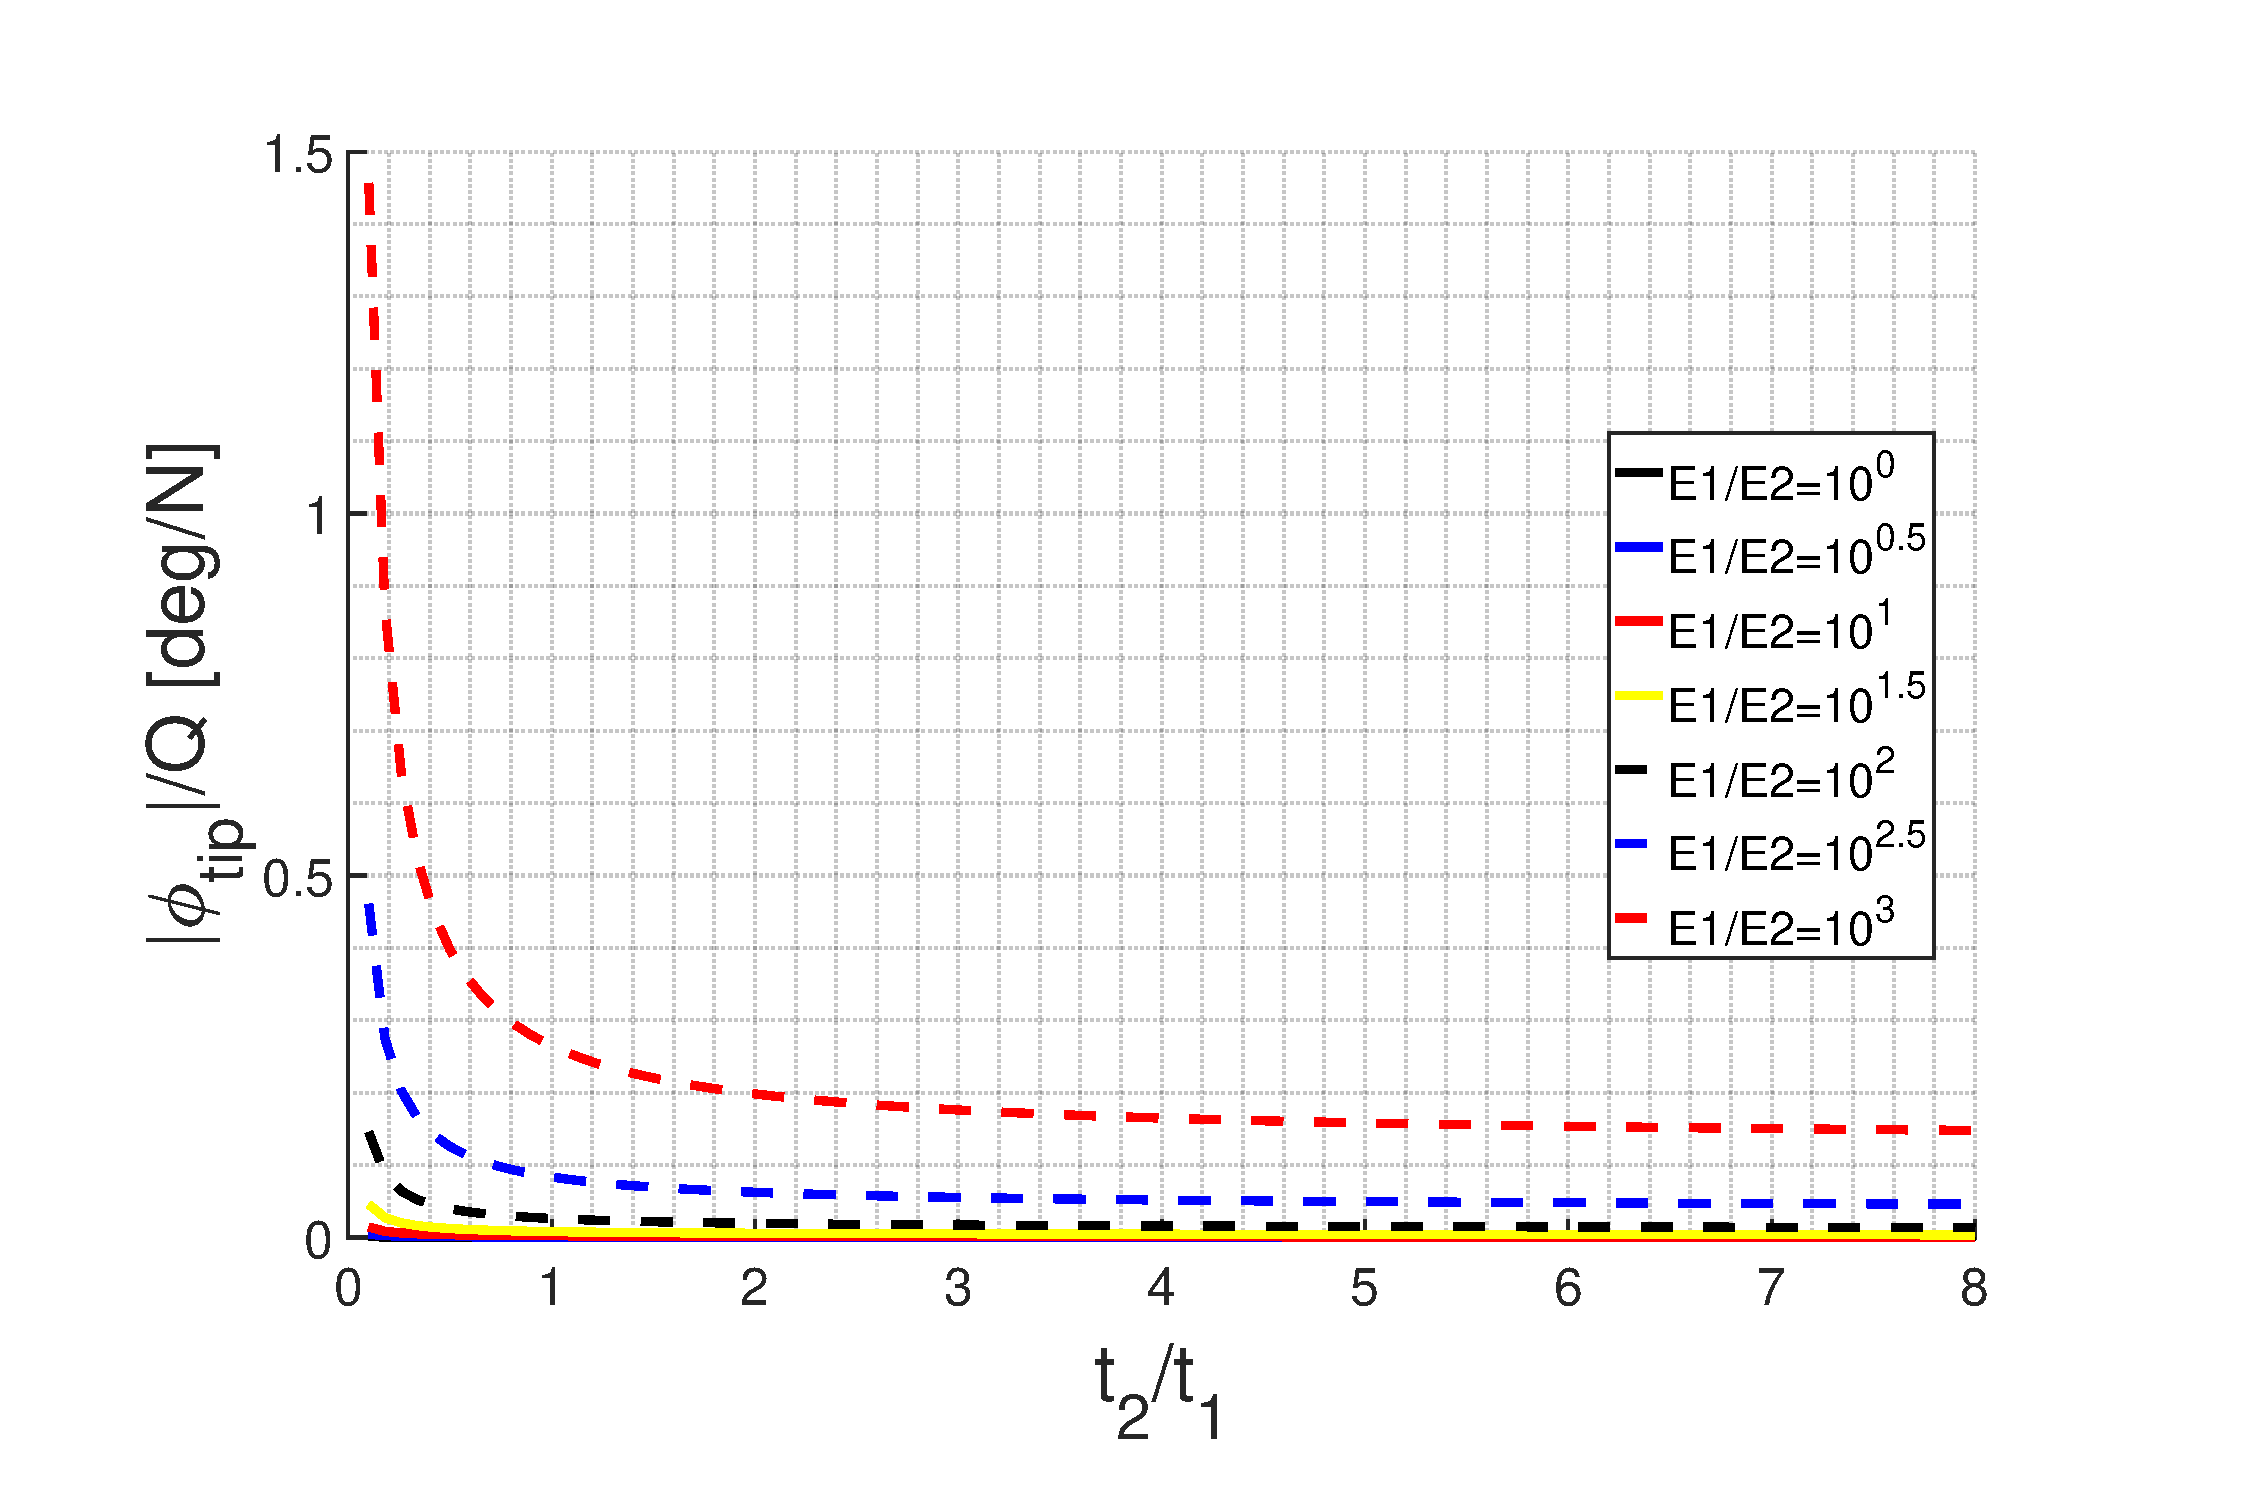
\includegraphics[width=0.8 \textwidth]{../analytical/figures/phioverQ-E1overE2-t2overt1}
      \caption[Influence of the thickness ratio $t2/t1$ on the torsional compliance]{Influence of the thickness ratio $t2/t1$ on the torsional compliance $|\phi_{\mathrm{tip}}| / Q$, shown for various values of the stiffness ratio $E_1/E_2$ ranging from $10^0$ to $10^3$. }\label{fig:phioverQ-E1overE2-t2overt1}
    \end{figure}

    \clearpage
    From the analysis of the torsional compliance $|\phi_{\mathrm{tip}}| / Q$ as a function of the thickness ratio $t_2/t_1$ in Figure \ref{fig:woverQ-E1overE2-t2overt1}, it can be seen that increments in $t_2/t_1$ amplifies the effects of variations of the stiffness ratio $E_1/E_2$ on the flexural compliance $w_{\mathrm{0,tip}} / Q$. On the other hand, Figure \ref{fig:woverQ-E1overE2-BoverH} shows that the flexural compliance $w_{\mathrm{0,tip}} / Q$ increases when the cross-sectional aspect ratio $B/H$ increases and the value of $B/H$ does not alter the magnitude of the effect of variations of $E_1/E_2$ in the flexural compliance, effect that remains small.

    From Figure \ref{fig:phioverQ-E1overE2-t2overt1}, it can be understood that there is not variation in the torsional compliance for values of the thickness ratio $t_2/t_1 > 1$; but for $t_2/t_1 < 1$, the torsional compliance increases considerably. This result shows again something similar at what it was shown in Subsection \ref{subsec:bendingTwistCoupling_results_model}, how the modification of shear stiffness in the second web has a considerable effect on the torsional stiffness. On the other hand, Figure \ref{fig:phioverQ-E1overE2-BoverH} shows small effect of the variation of the cross-sectional aspect ratio $B/H$ on the torsional compliance.

    The effect of the slenderness ratio $L/B$ on the deflection and torsional compliances is shown in Figures \ref{fig:woverQ-E1overE2-LoverB} and \ref{fig:phioverQ-E1overE2-LoverB}, respectively. These two figures show how the flexural and torsional compliance increase for increasing values of $L/B$. Also, Figure \ref{fig:woverQ-E1overE2-LoverB} shows again the small influence of the stiffness ratio $E_1/E_2$ in the flexural compliance while Figure \ref{fig:phioverQ-E1overE2-LoverB} shows how the torsional compliance is considerably affected by variations of $E_1/E_2$.

    %%%% Figures variation of L / B
    \begin{figure}[!htpb] %w_0,tip / Q versus L/B, flexural compliance
      \centering
      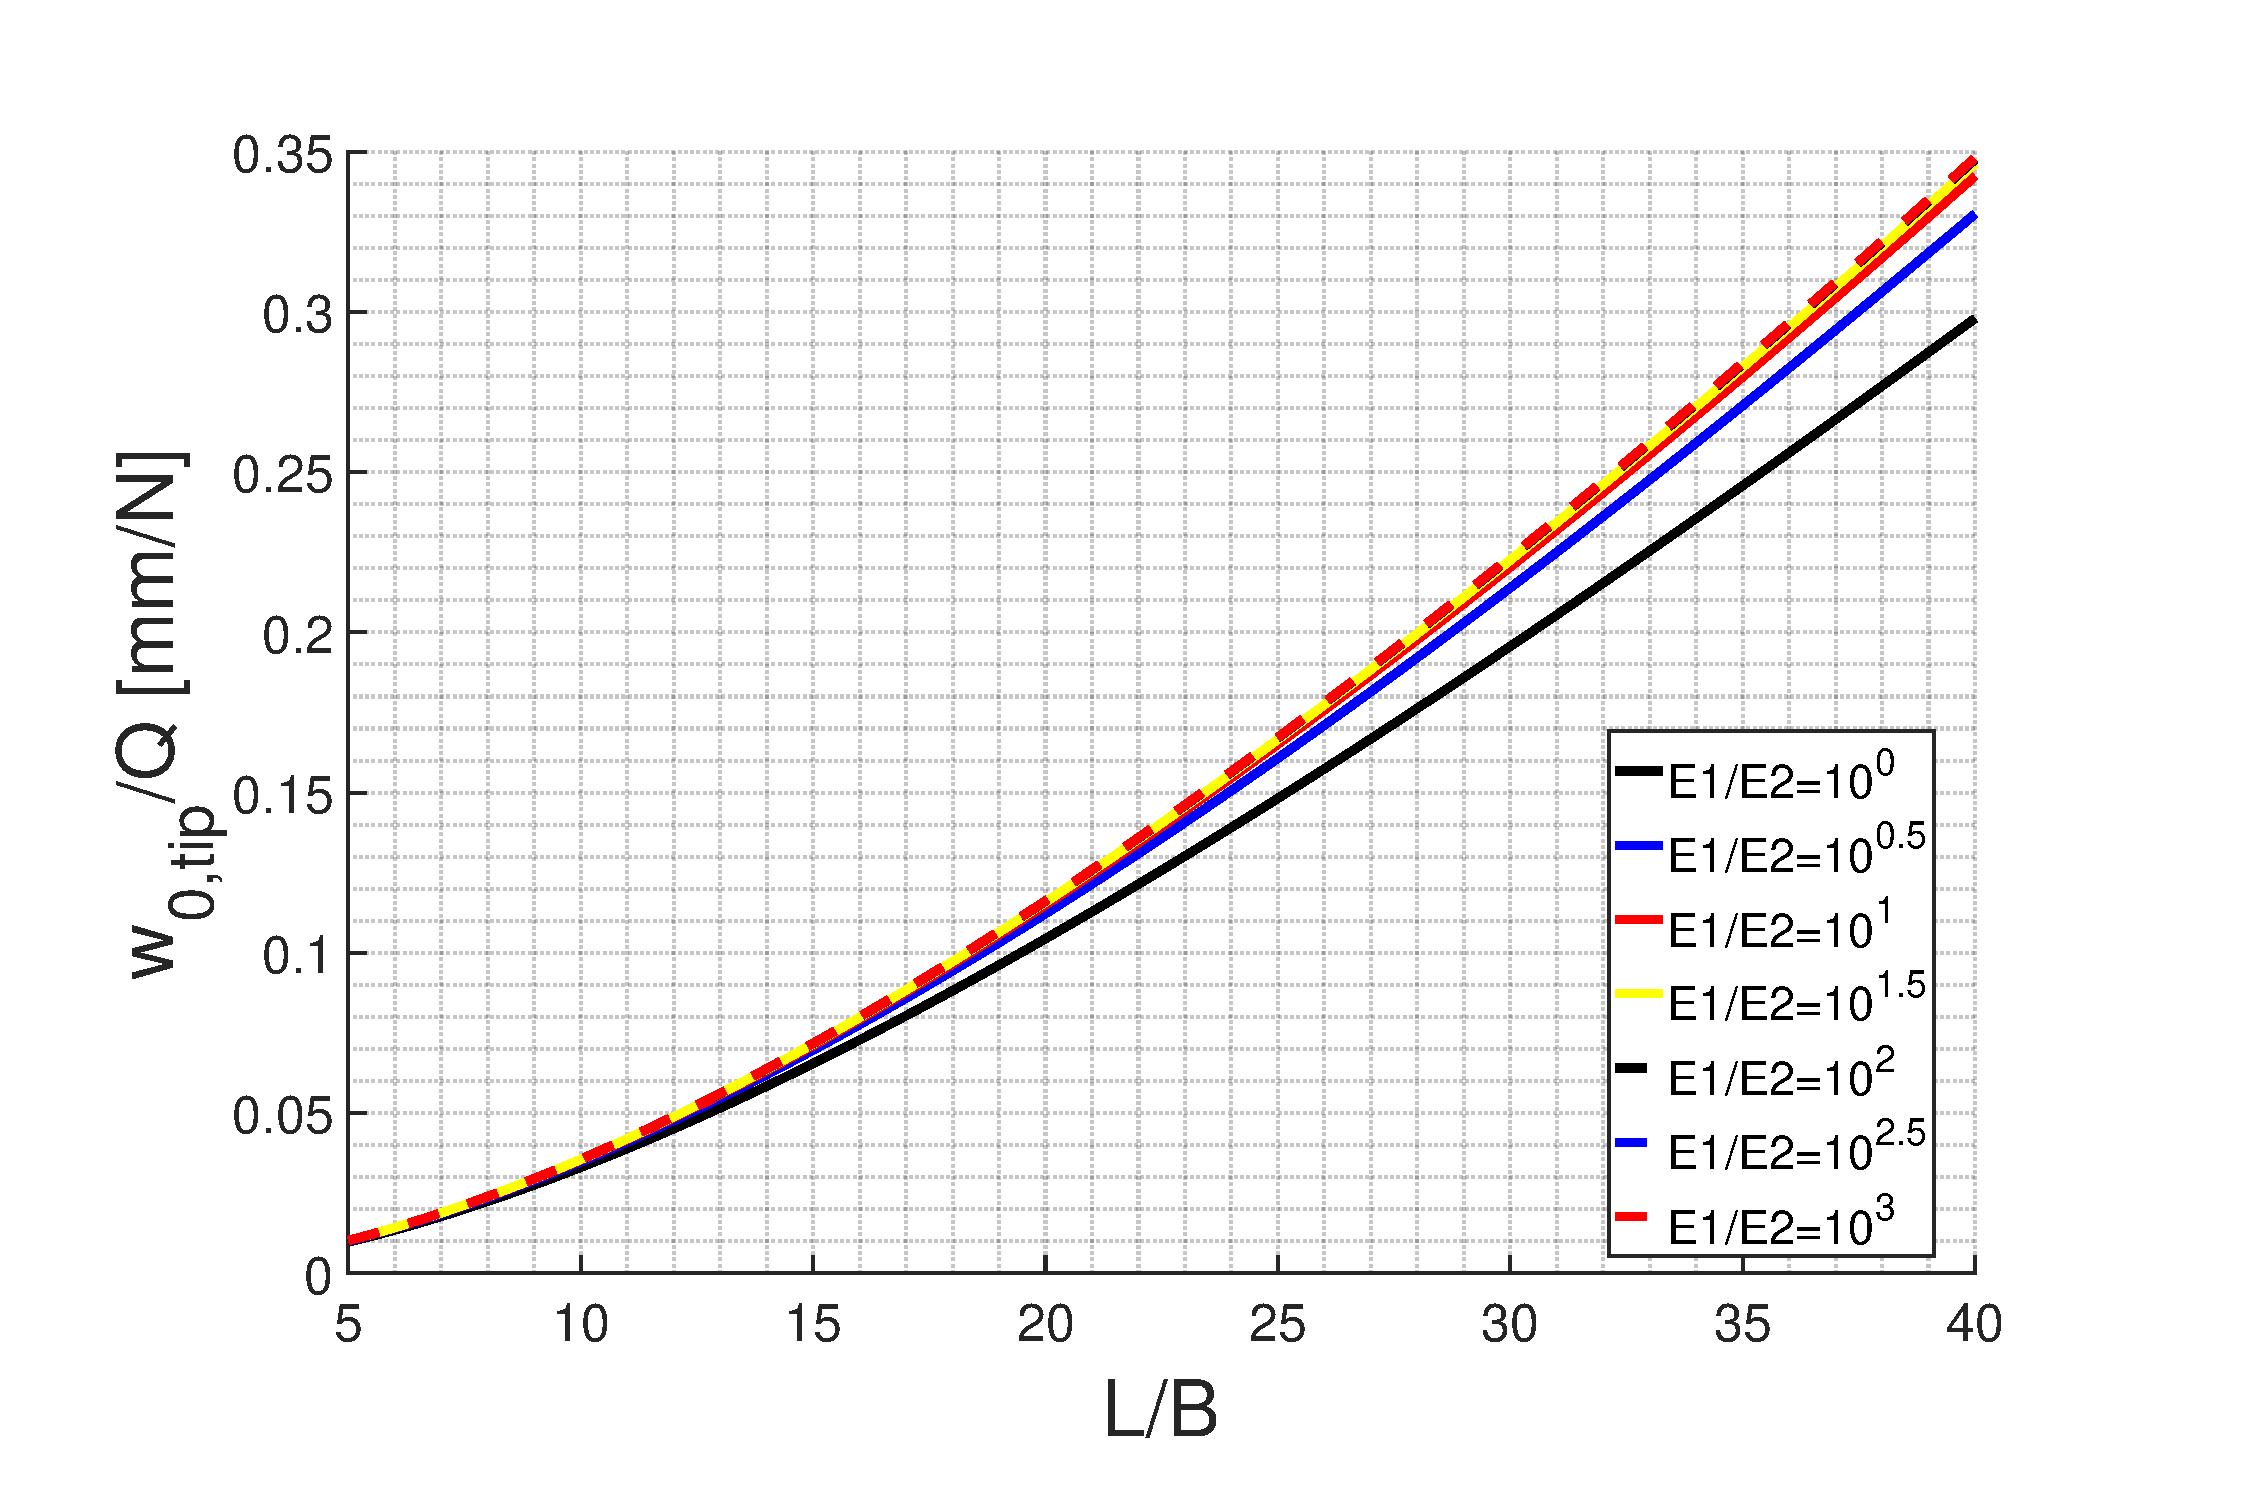
\includegraphics[width=0.8 \textwidth]{../analytical/figures/woverQ-E1overE2-LoverB}
      \caption[Influence of the slenderness ratio $L/B$ on the flexural compliance]{Influence of the slenderness ratio $L/B$ on the flexural compliance $w_{\mathrm{0,tip}} / Q$, shown for various values of the stiffness ratio $E_1/E_2$ ranging from $10^0$ to $10^3$. }\label{fig:woverQ-E1overE2-LoverB}
    \end{figure}

    \begin{figure}[!htpb] %\phi_tip / Q versus L/B, torsional compliance
      \centering
      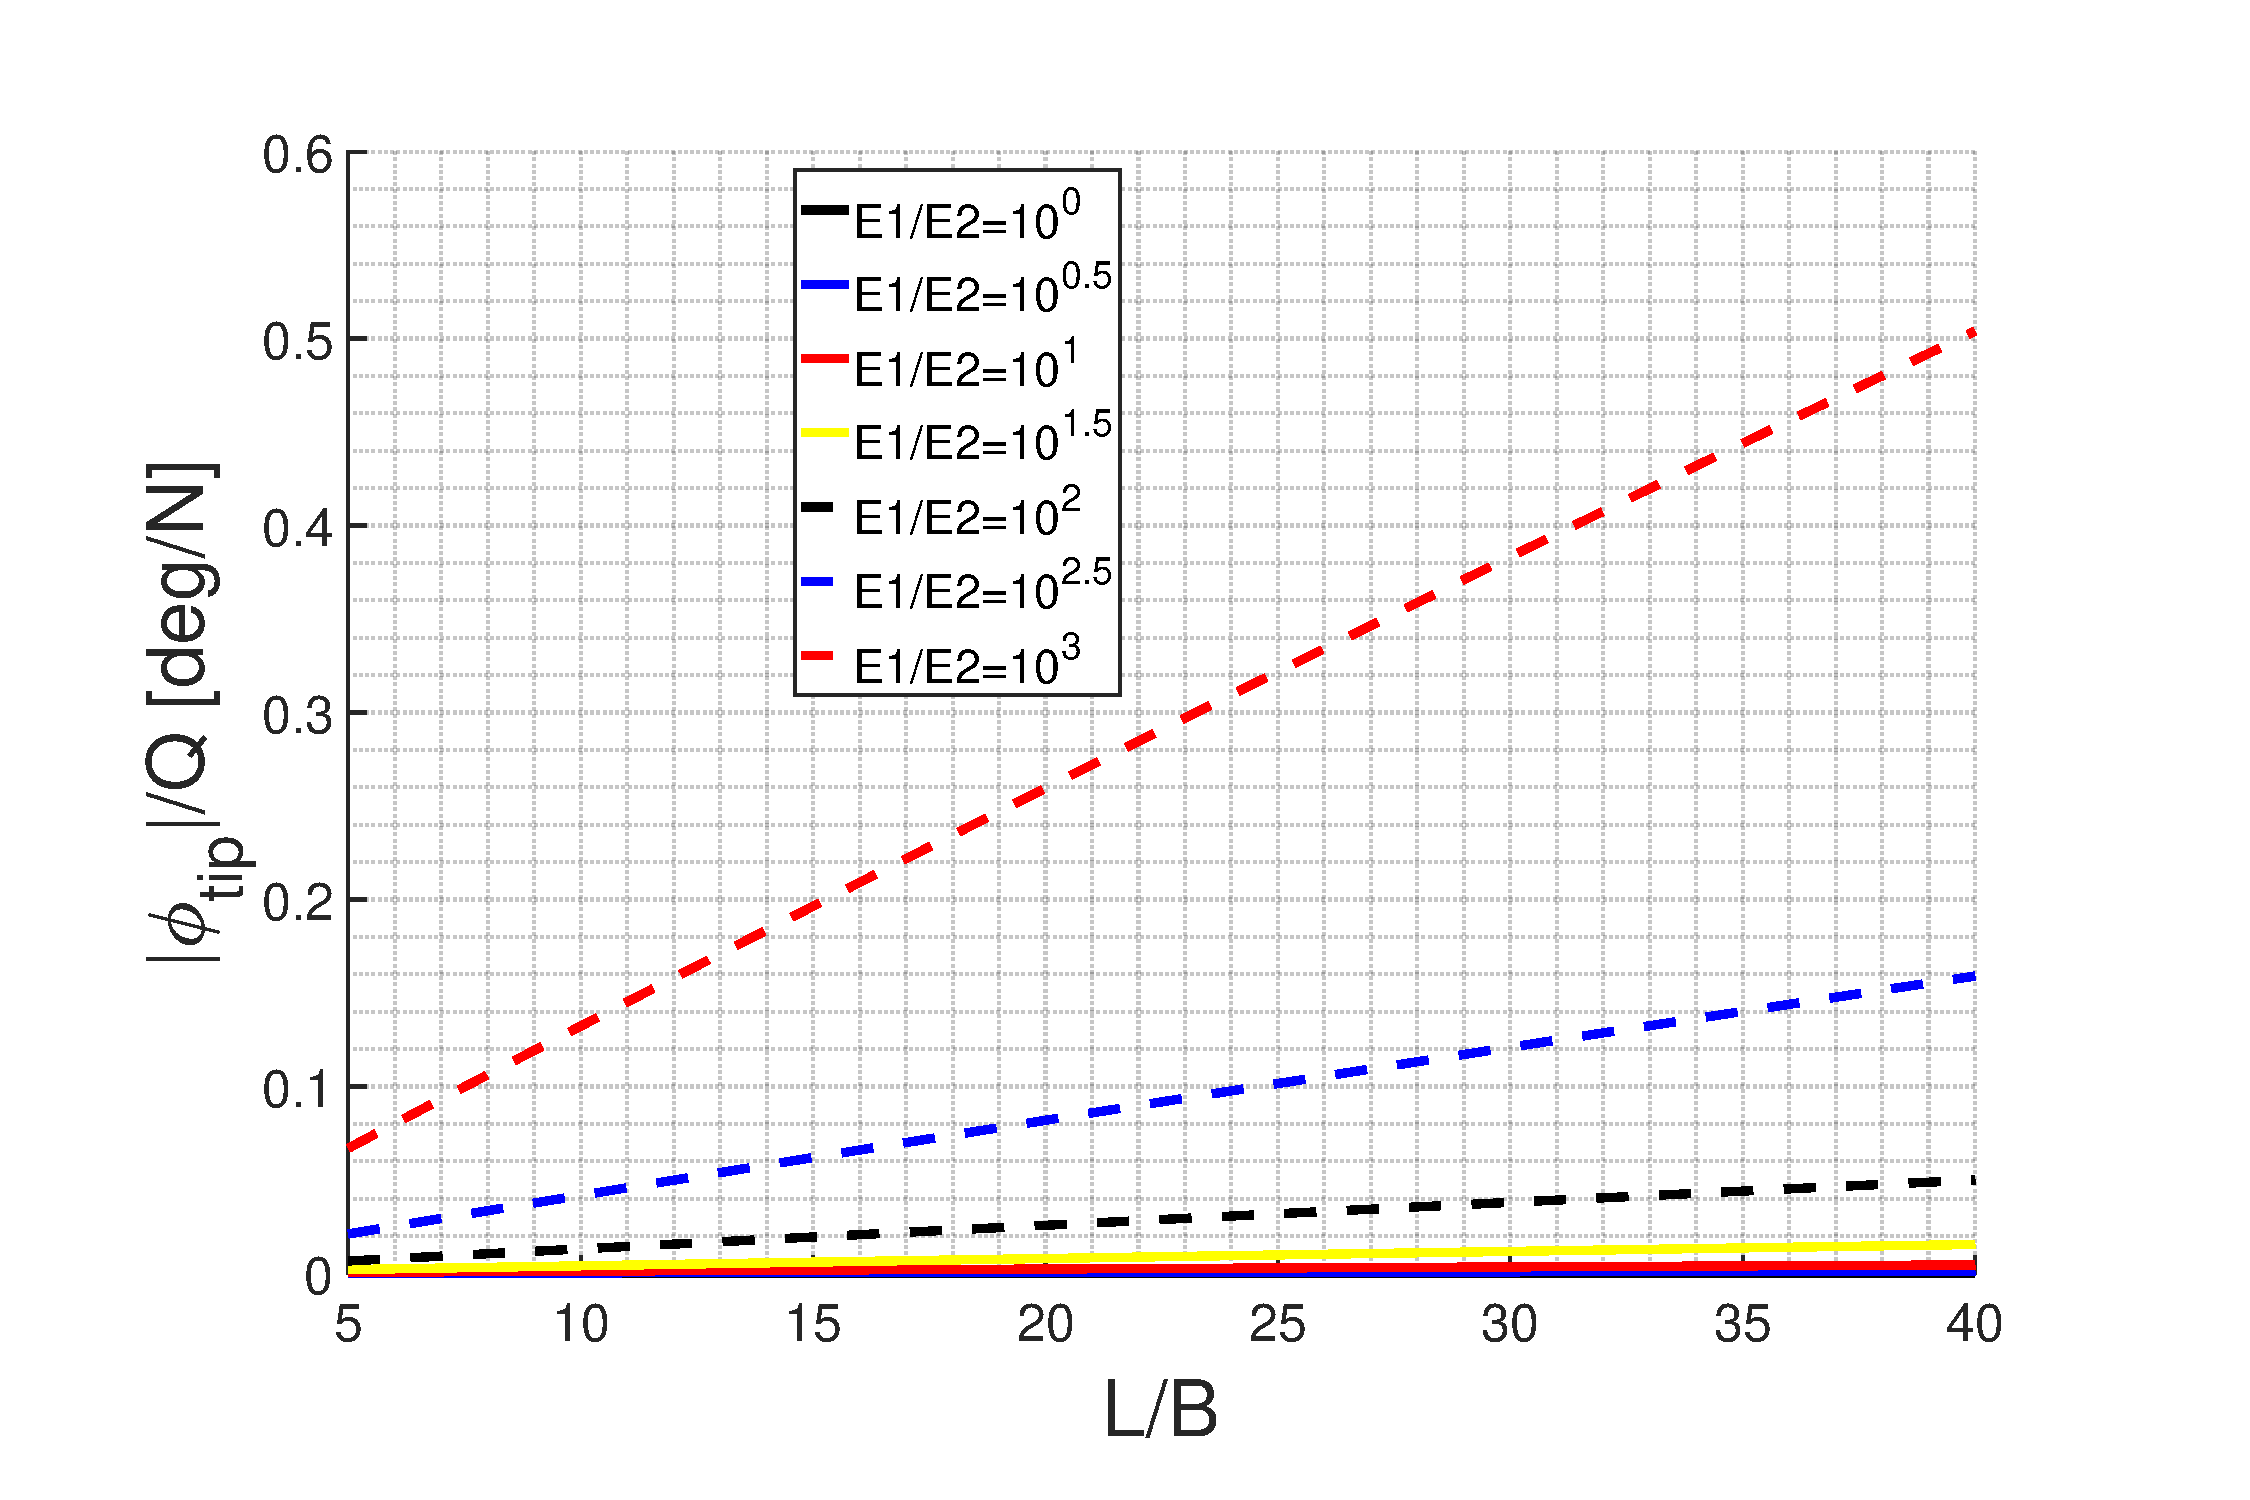
\includegraphics[width=0.8 \textwidth]{../analytical/figures/phioverQ-E1overE2-LoverB}
      \caption[Influence of the slenderness ratio $L/B$ on the torsional compliance]{Influence of the slenderness ratio $L/B$ on the torsional compliance $|\phi_{\mathrm{tip}}| / Q$, shown for various values of the stiffness ratio $E_1/E_2$ ranging from $10^0$ to $10^3$. }\label{fig:phioverQ-E1overE2-LoverB}
    \end{figure}

\clearpage
\section{Computational model analysis} \label{sec:computationalModelAnalysis_results_model}

  In the present section, results from the analysis performed on the computational model are presented. Different aspects of the model are evaluated and design decisions are justified. The analysis considers the modeling of the lattice nodes rigid behavior, the different load introduction strategies, the influence of the mesh in the simulation convergence, the addition of the ribs and the nonlinearities that appear in the problem.

  For the proposed technology, it is expected to see the appearance of large deformations and elastic instabilities in the structure. This means that the structural stiffness of the model is altered as the load applied increases. For this reason, it becomes necessary to execute nonlinear simulations in which the load applied is increased by small step increments. Each of these steps constitutes a different frame that contains particular values of the problem magnitudes at the mesh nodes and elements.

  Furthermore, linear simulations are also executed to provide information of the expected response of the structure considering its initial stiffness, before the onset of the elastic instabilities that alter the stiffness. The results obtained from the nonlinear simulations are compared to those obtained from the linear simulations. This comparison is done by means of the curve displacement-force that shows the achieved twist adaptation of the wing-box at each of the frames that build up the complete simulation window.

  In addition to this general nonlinear/linear global response comparison, the performance of the structure is also analysed by means of the evaluation of the six possible displacements of the mesh nodes at different parts of the structure. The value of these magnitudes are shown in colour contours plots over the solution model.

  % \subsection{Connection between the chiral lattice and the wing-box skin} \label{subsec:connection_results_model}
  %
  %   The modeling of the lattice nodes through either the coupling through a reference point and through tyre was shown to
  %
  %For the parametric study that was performed this reason, it was decided not to use a model where the connection between the chiral lattice and the wing-box skin is modeled following the approach exposed in the Subsection \ref{subsec:connections_computationalModel}. Instead, a more rough connection is used, as shown in Figure \ref{fig:connectionSimple}.
  %
  %    \begin{figure}[!htpb]
  %      \centering
  %      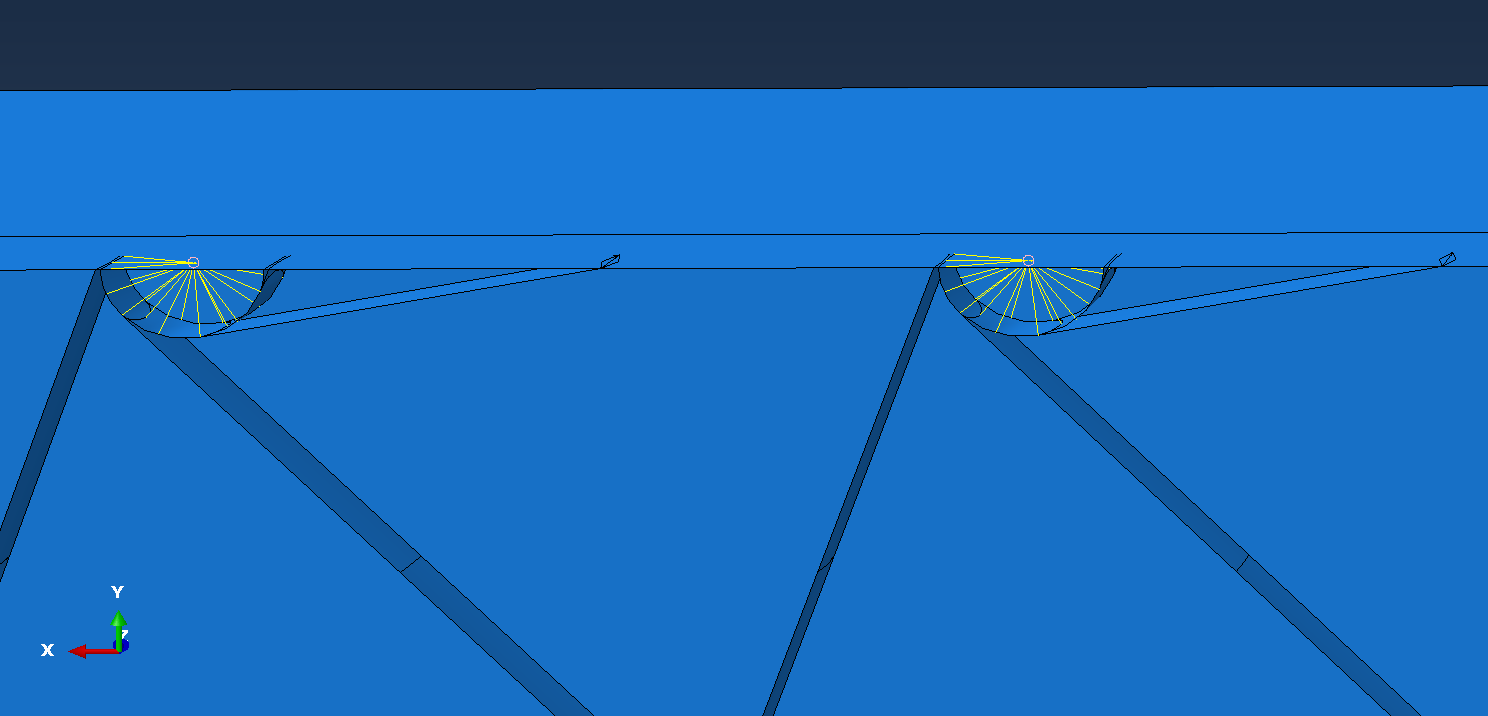
\includegraphics[width=0.8 \textwidth]{figures/result-model/connectionSimple}
  %      \caption[Connection between the chiral lattice and the wing-box for the parametric study]{Connection between the chiral lattice and the wing-box for the parametric study.}\label{fig:connectionSimple}
  %    \end{figure}
  %
  \subsection{Rigid body modeling} \label{subsec:rigidBody_results_model} %To be reviewed
    % -> Rotation of the nodes was like 20\% inferior with the coupling
    
    Two different approaches are followed to model the rigid body behavior of the lattice nodes, as it has been already explained in Subsection \ref{subsec:latticeNodesRigid_Parametrization}. The first modeling approach considers the creation of a coupling condition between a reference point positioned at the centre of the lattice node cylinder and mesh nodes located in the faces of the lattice node. The second approach consists on the introduction of an additional part that is placed in the middle of the cylinder to add stiffness to the element. In this section, the results obtained for each modeling approach are compared.

    In Figure \ref{fig:rigid-modeling}, the displacement-force curve for the nonlinear and linear responses in wing-box twist obtained for each modeling approach are compared. It can be seen that when the tyre approach is used, the collapse of the structure occurs at a smaller load than if the coupling implementation is used.

    Also, the analysis of the mesh nodes displacements on the solution model shows that, when the tyre rigid body behavior is modeled using the tyre part, the rotation of the lattice nodes around its own axis is approximately 20\% higher than when the modeling is done using the coupling constraint. This rotation should be free and be only constrained by the connection to the ligaments. Therefore, it is concluded that the use of the tyre part is a more realistic approach to modeling the rigid body behavior of the lattice nodes.

    \begin{figure}[!htpb]
      \centering
      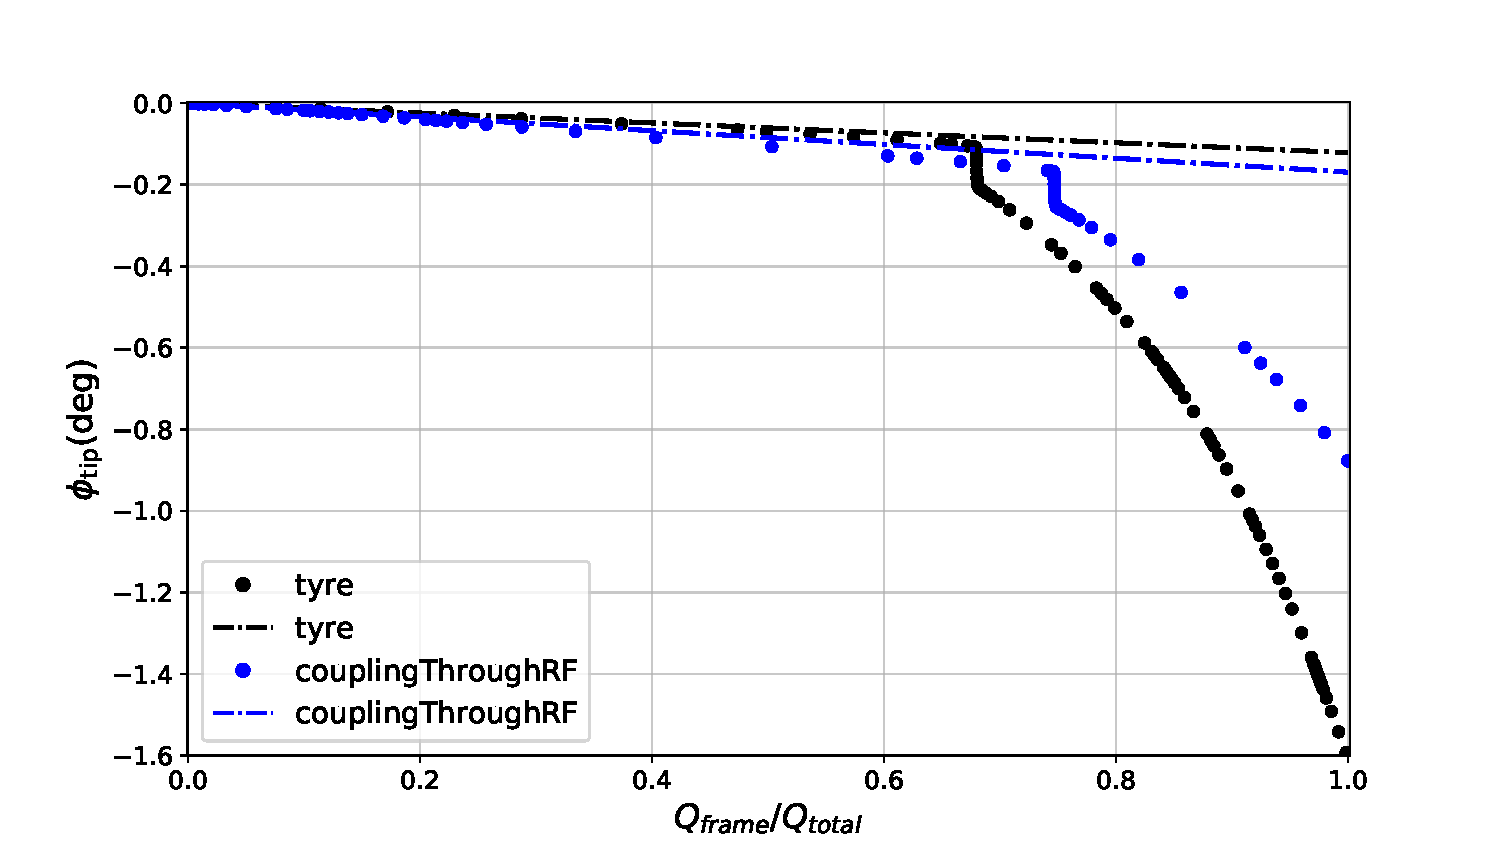
\includegraphics[width=0.8 \textwidth]{figures/result-model/rigid-modeling}
      \caption[Displacement-force curve obtained using different approaches to model the rigid lattice node]{Displacement-force curve obtained using different approaches to model the rigid lattice node. }\label{fig:rigid-modeling}
    \end{figure}

  \clearpage
  \subsection{Load introduction method} \label{subsec:load_results_model}

    As shown in Subsection \ref{subsec:load_computationalModel}, there are multiple ways in which the load can be introduced into the structure. It was decided to locate the load introduction points at the upper flange of the ribs in an attempt of replicate how the load will be introduced in a future manufactured demonstrator. In this subsection, the different results obtained when modifying the load introduction method are shown. 

    Firstly, the option of distributing the same total load over the total number of ribs, three in the baseline configuration, is compared with the option of concentrating all the load on the upper flange of the tip rib. In Figure \ref{fig:forceDisplacement-distributedLoad700N}, the curve displacement-force is shown for these two different cases. It can be seen how when the load is distributed over a number of points and it is not concentrated on a single point, a delay in the onset of the structure collapse occurs. This result is correlated with visual inspection of the displacement of the mesh nodes on the solution model in Abaqus. The corresponding colour contour of the rotational total displacement $\sqrt{\theta^2 + \phi^2 + \psi^2}$ for a distributed load is shown in Figure \ref{fig:distributedLoad700N}. Here it can be seen how buckling has started to occur on the ligaments located close to the ribs, where the load is being introduced. In a further stage, when load increases, buckling would start to occur at the root of the wing-box.

    \begin{figure}[!htpb]
      \centering
      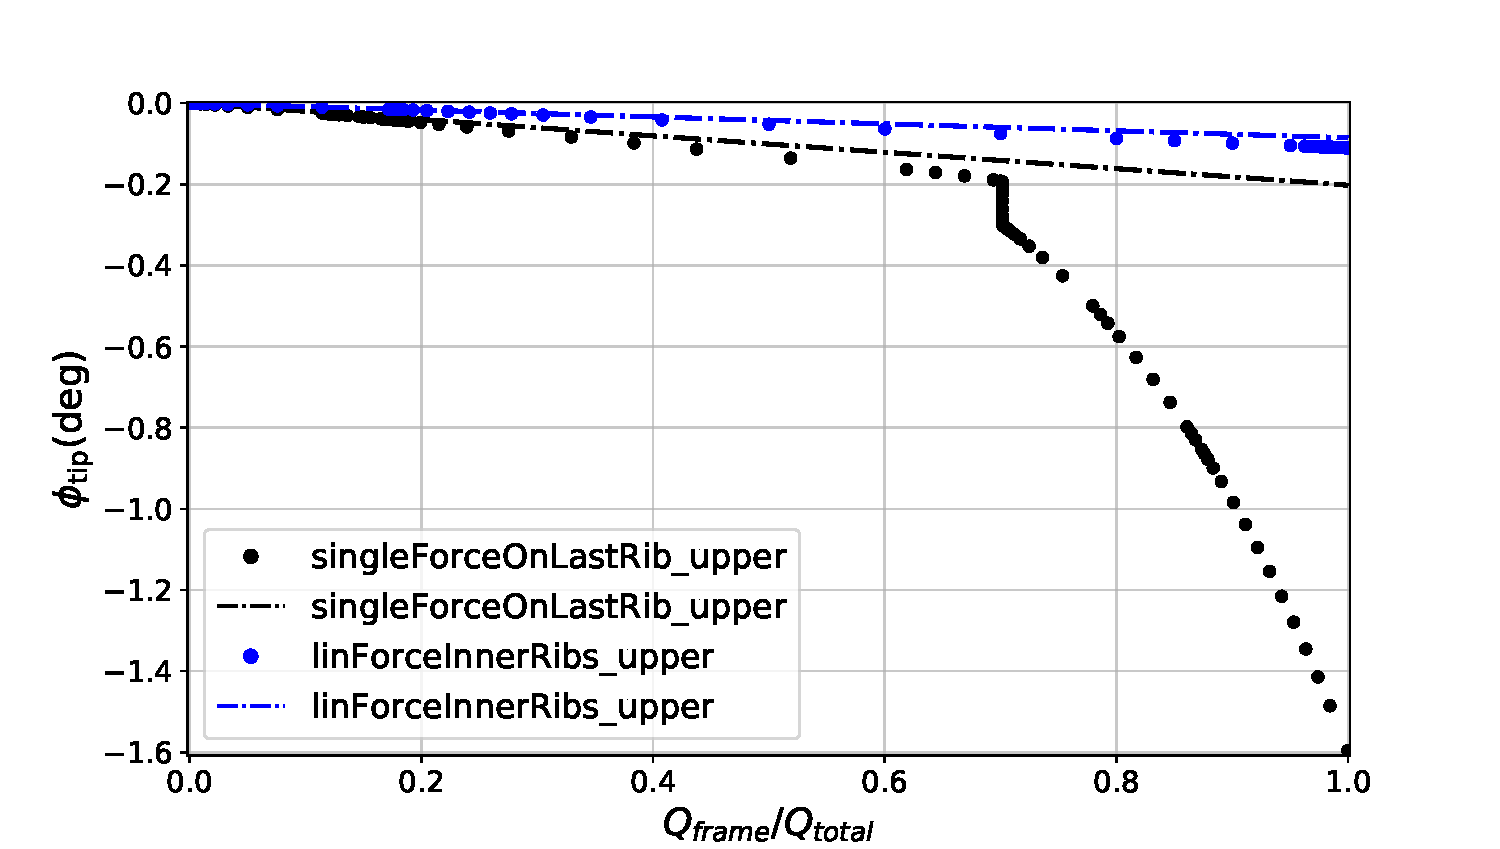
\includegraphics[width=0.8 \textwidth]{figures/result-model/forceDisplacement-distributedLoad700N}
      \caption[Displacement-force curve showing the model response using different load introduction methods]{Displacement-force curve showing the model response using different load introduction methods. The label ``singleForceOnLastRib\_upper'' corresponds to the case of using one single point for the load introduction. This point is located at the upper flange of the tip rib. The label ``linForceInnerRibs\_upper'' corresponds to the case of introducing load on the upper flange of all the available ribs, which are three for the baseline configuration, two in the inner part of the wing-box and one at the tip. It can be see that the concentration of the load advances the onset of the structure collapse.}
      \label{fig:forceDisplacement-distributedLoad700N}
    \end{figure}

    \begin{figure}[!htpb]
      \centering
      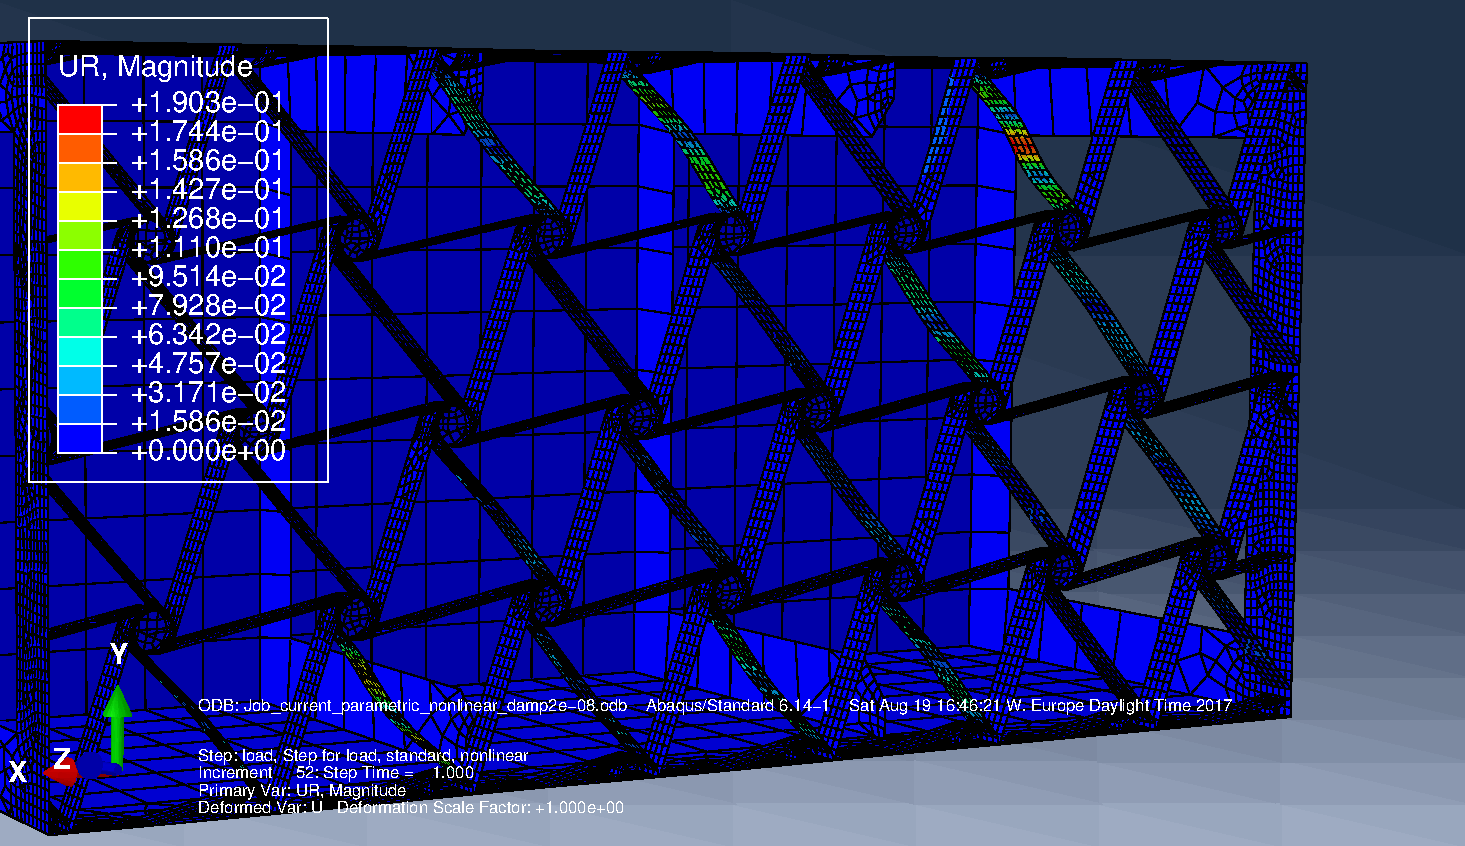
\includegraphics[width=0.8 \textwidth]{figures/result-model/distributedLoad700N}
      \caption[Deformed state of the model for a distributed load introduction method]{Deformed state of the model for a distributed load introduction method. It can be seen how since the buckling is starting to occur at the ligaments located close to the ribs, the onset of the elastic instabilities is delayed.}
      \label{fig:distributedLoad700N}
    \end{figure}

    Secondly, in Figure \ref{fig:forceDisplacement-loadZ0coma8} a comparison of the response for different load position points in the chordwise direction is shown. The plot shows the displacement-force curve for four values of the variable $z/W_{\mathrm{box}}$. A smaller value of $z/W_{\mathrm{box}}$ represents a load introduction point located closer to the chiral lattice. It can be seen that buckling is not triggered for values of $z/W_{\mathrm{box}}$ equal to 0.6 and 0.8. This is explains because the further the introduction point is from the chiral lattice, the less shear strain appears on the chiral lattice and the later that the onset of the elastic instabilities occurs. 

    Since the distribution of the load in more that one rib only delays the onset of the instabilities, it is decided to use a single load introduction point for the study performed on the baseline configuration, in a attempt to simplify the model. Also, it is decided to locate the load introduction point at $z/W_{\mathrm{box}} = 0.5$ to keep the symmetry.

    \begin{figure}[!htpb]
      \centering
      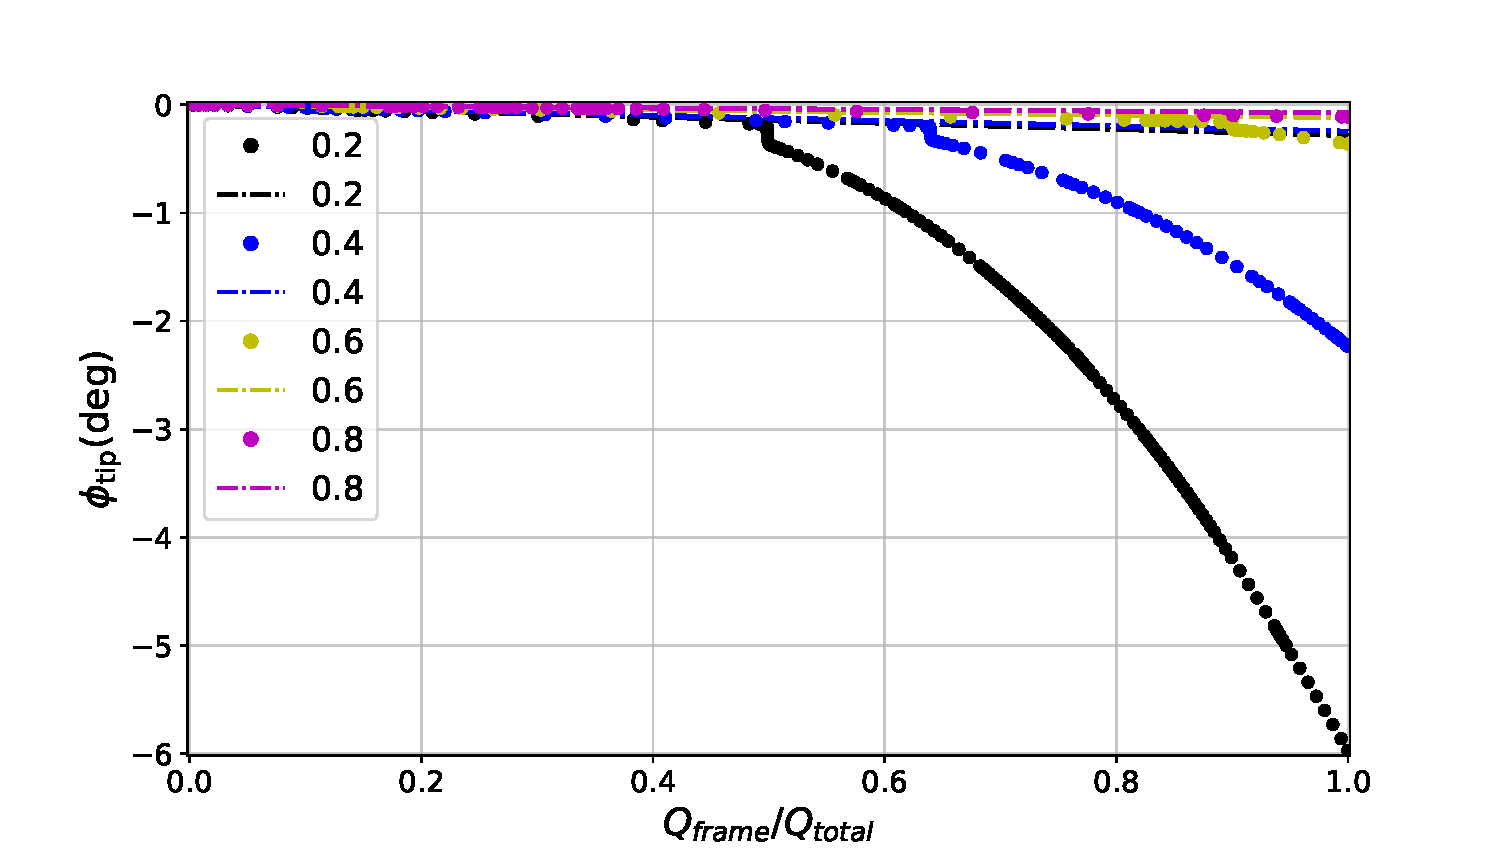
\includegraphics[width=0.8 \textwidth]{figures/result-model/forceDisplacement-loadZ0coma8}
      \caption[Displacement-force curve showing the model response for different load introduction points $z/W_{\mathrm{box}}$]{Displacement-force curve showing the model response for different load introduction points $z/W_{\mathrm{box}}$. A smaller value of $z/W_{\mathrm{box}}$ represents a load introduction point located closer to the chiral lattice. The further the introduction point is from the chiral lattice, the less shear strain appears at the chiral lattice and the later that the onset of the elastic instabilities occurs.}
      \label{fig:forceDisplacement-loadZ0coma8}
    \end{figure}

  \clearpage
  \subsection{Connection between the wing-box skin and the chiral lattice} \label{subsec:connection_results_model} %To be reviewed

    As it has been already explained in Subsection \ref{subsec:connections_computationalModel}, the modeling of the connection between the chiral lattice structure and the wing-box skin is one of the critical aspects of the design. In the basic connection type, the lattice node is cut by half and it is directly attached to the wing-box skin, restraining all the possible degrees of freedom. In a further step, the lattice node is allowed to rotate around its own axis. For this type of connection,  the rotational displacement $\theta$ of the mesh node in the centre of the tyre embedded into the lattice node is left uncoupled when defining the coupling constraint with the mesh nodes on the wing-box skin. Additionally, it is also possible to allow the lattice node to translate parallel to the wing-box skin, leaving the degree of freedom $u$ unrestrained.

    In Figure \ref{fig:UR1_tau-additionalBCAll}, the displacement-force curves obtained for the three types of connection are shown. It can be seen how allowing the free rotation of the nodes leads to an earlier onset of the instabilities that causes the structure collapse. Additionally, it can be seen that when the displacement $u$ is left unrestrained, the mechanism activation occurs even before. In in case, the 

    Finally, the total rotational displacement of the mesh elements is shown in a colour contour plot in Figure \ref{fig:connectionUR3}, where it can be seen how a different buckling field appears for each of the modeling approaches. 

    \begin{figure}[!htpb]
      \centering
      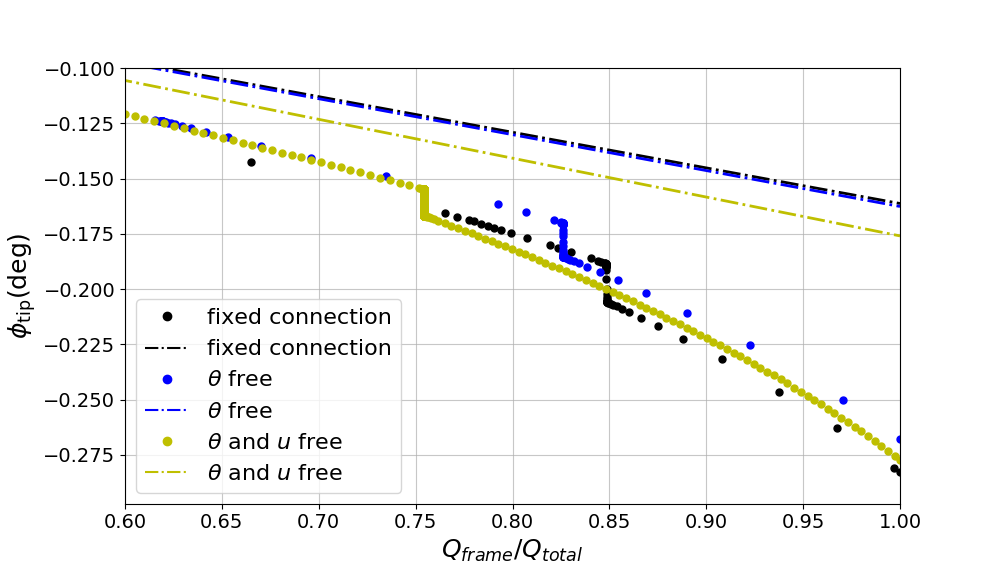
\includegraphics[width=0.8 \textwidth]{figures/further/UR1_tau-additionalBCAll}
      \caption[Displacement-force curve showing the model response for different approaches to model the connection between the chiral node and the wing-box skin]{Displacement-force curve showing the model response for different approaches to model the connection between the chiral node and the wing-box skin. The label ``fixed connection'' represents the wing-box twist adaptation obtained when creating a fixed connection while the label ``free rotation'' represents the wing-box twist adaptation when rotation of the lattice node is left unrestrained. The allowance of free rotational displacement $\theta$ of the lattice nodes around its own axis provokes the advance of the onset of the instabilities.}
      \label{fig:UR1_tau-additionalBCAll}
    \end{figure}

    \begin{figure}[!htpb]
      \centering
      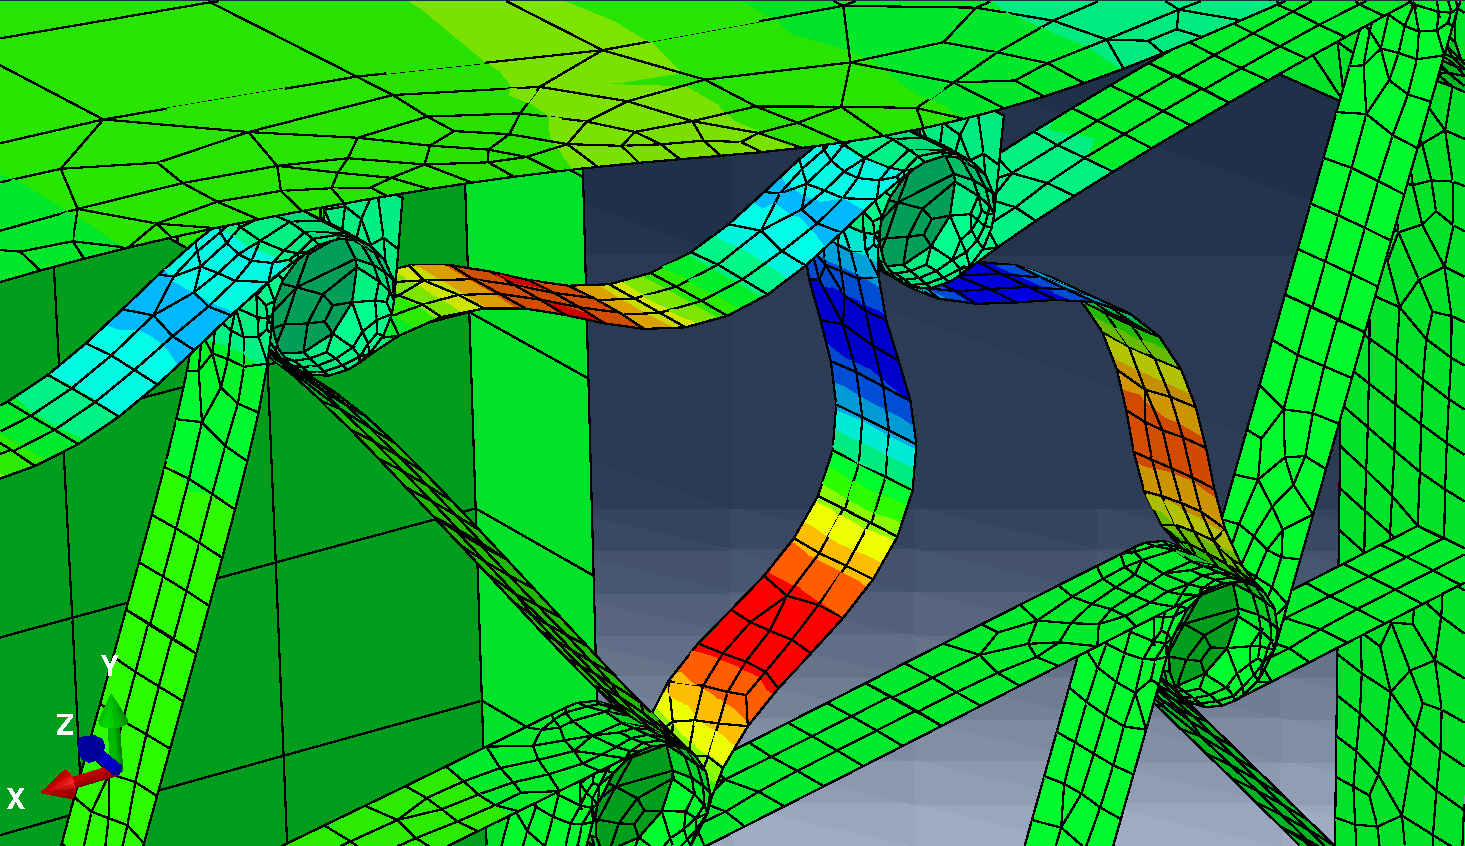
\includegraphics[width=0.8 \textwidth]{figures/further/connectionUR3}
      \caption[Color contour representation of the total angular displacement of the mesh elements on the deformed structure for different approaches to model the connection between the chiral node and the wing-box skin]{Color contour representation of the total angular displacement of the mesh elements on the deformed structure for different approaches to model the connection between the chiral node and the wing-box skin. The figure on the right shows the buckling field when the connection is such that the lattice nodes are restrained in all its degrees of freedom, and the one in the left shows the buckling field when the rotation of the lattice nodes is allowed. It can be seen how different connection approaches load to different buckling fields.}
      \label{fig:connectionUR3}
    \end{figure}

  \clearpage
  \subsection{Mesh} \label{subsec:mesh_results_model}

    The model is build using cell shell elements as the fundamental constituting part. The thickness is assigned in the perpendicular direction, as it is shown in Figure \ref{fig:shellElement}.

    This type of element is a 2D element that it was used to build 3D structures. This kind of procedure may incur in distortions in the mesh elements due to shell elements intersecting in the same line at different angles. For the designed model, this situation occurred at certain locations of the chiral lattice structure. It can be seen in Figure \ref{fig:meshDistorted} that the distorted elements appear at two different locations. Firstly, at the plane where the two ligaments with different curvature join. At this point, the sharp angles that appear in between the geometrical lines induce the appearance of tetrahedral distorted mesh elements. The second typical location for appearance of distorted elements is along the curve where the lattice nodes and the curved ligaments join.

    \begin{figure}[!htpb]
      \centering
      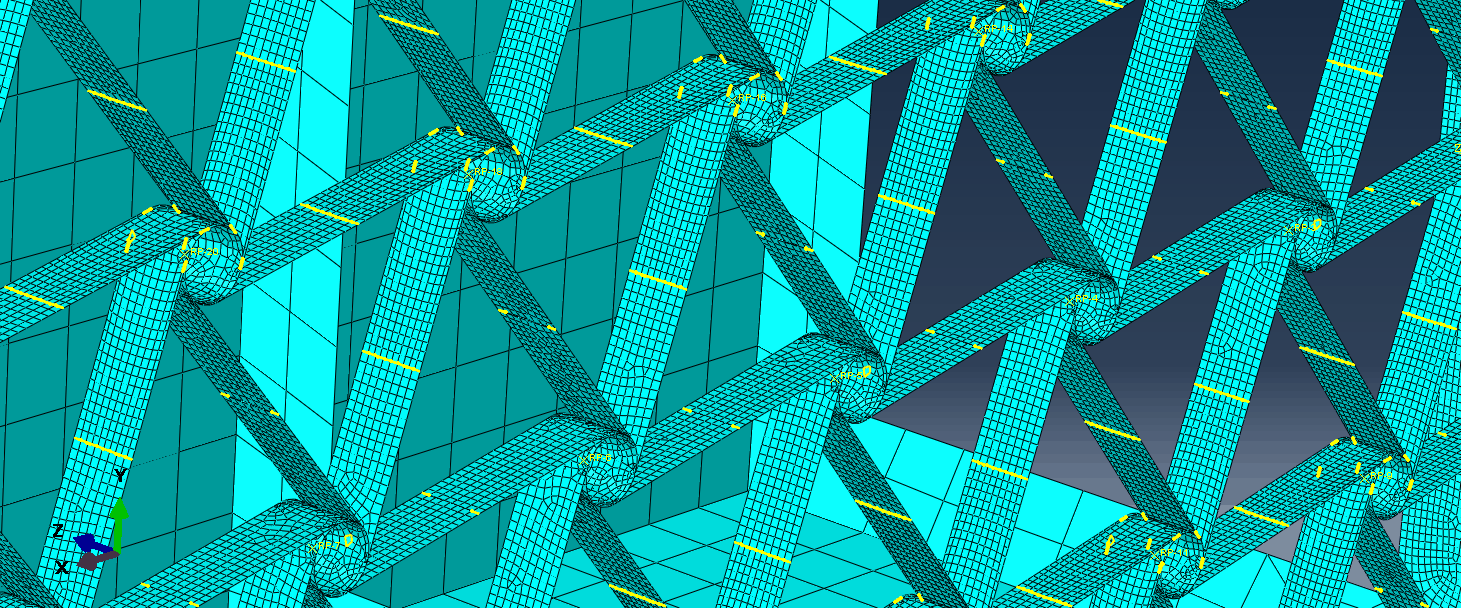
\includegraphics[width=0.8 \textwidth]{figures/result-model/meshDistorted}
      \caption[Distorted mesh elements in the model]{Distorted mesh elements in the model. The number of distorted elements was found to be crucial for the simulation convergence.}\label{fig:meshDistorted}
    \end{figure}

    It was seen that the number of distorted elements had a significant effect in the simulation convergence evolution. For a high number of distorted elements, the simulation could not go further from the first step. No attempts to locally modify the mesh at the mentioned locations were made, instead, it was found that modifying the global mesh size gave enough control over the number of distorted elements to be able to overcome this limitation. The bigger the mesh size in the area, the less distorted elements appear after completing the meshing operations.

  \clearpage
  \subsection{Nonlinear problem and automatic stabilization} \label{subsec:nonlinear_results_model} %OK

    For the case under study, nonlinear simulations are carried out as is expected to find large displacement and non-constant stiffness. In Abaqus, to execute nonlinear simulation involves the following considerations, as shown in \cite{Abaqus}:
    %
    \begin{itemize}
      \item a combination of incremental and iterative procedures;
      \item using the Newton method to solve the nonlinear equations;
      \item determining convergence;
      \item defining loads as a function of time; and
      \item choosing suitable time increments automatically.
    \end{itemize}

    Therefore, Abaqus breaks the step where the load is applied into increments. The software automatically chooses the size of each of the increments based on the convergence evolution of previous increments.

    Also, nonlinear static problems may become unstable. One of the possible sources of such instabilities is buckling. A model where buckling appears locally may not be resoluble using general solution methods. For this kind of cases, it becomes necessary to either solve the problem dynamically or with the aid of artificial damping.

    Since the above situation represents what it is expected to be found in the model response, a constant artificial damping factor is used throughout the whole step to account for the appearance of local instabilities.

    \noindent
    Automatic stabilization with a constant damping factor implies that viscous forces of the form:
    \begin{equation}
      F_v = c \mat{M} v
    \end{equation}
    are added to the global equilibrium equations:
    \begin{equation}
      P - I - F_v = 0,
    \end{equation}
    %
    where $I$ represents the internal forces, $P$ the external forces, $\mat{M}$ is the artificial mass matrix calculated with unity density, $c$ is the defined damping factor, $v = \Delta u / \Delta t$ is the vector of nodal velocities, and $\Delta t$ is the increment of simulation time.

    The final value of $c$ that is going to be used during the simulations is chosen after performing a small parametric study of the different possibilities. As a result, the plot shown in Figure \ref{fig:forceDisplacement-damp} is produced. This plot represents the evolution of the twist at the tip as the load is increased step by step during the nonlinear simulation. As it will be explained in Section \ref{sec:generalResponseCharact_results_sim}, the use of automatic stabilization becomes necessary to capture the nonlinear mechanics that involve buckling on the chiral ligaments and the ultimate collapse of the structure. Finally, special care needs to be taken in order to ensure that the inclusion of artificial damping factor is not leading to inaccurate results due to over-damping of the structure. This can be done by comparing the fraction of the static energy that it is dissipated compared with the external work that is introduced into the system. Such a comparison is presented in the discussion below.

    \begin{figure}[!htpb]
      \centering
      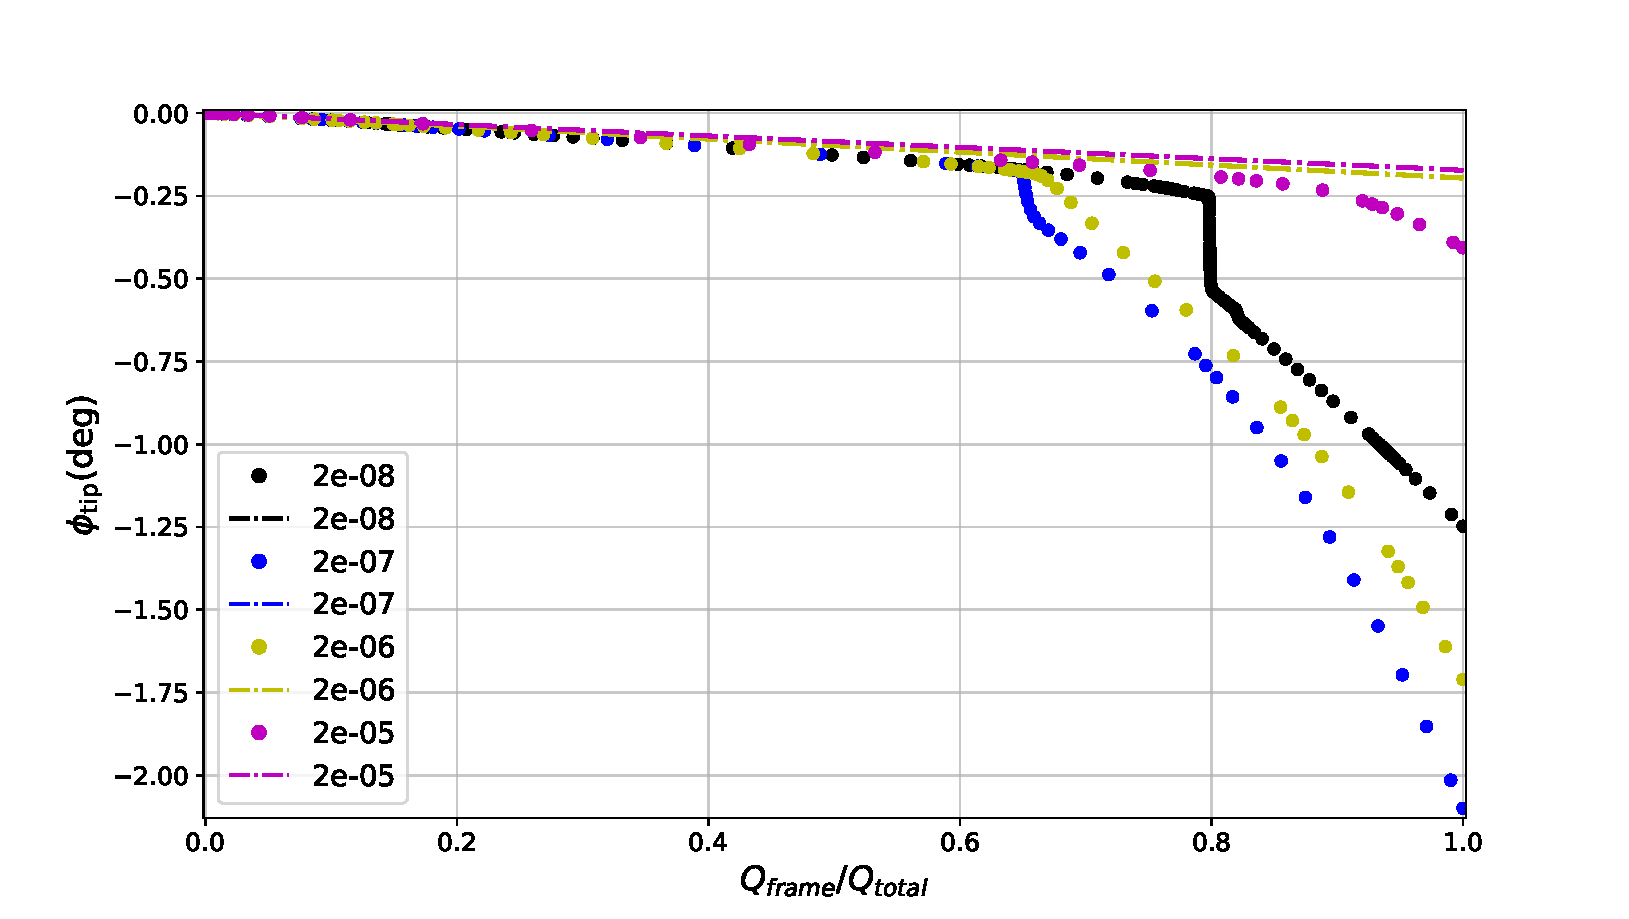
\includegraphics[width=0.8 \textwidth]{figures/result-model/forceDisplacement-damp}
      \caption[Displacement-force curve for various values of constant artificial damping factor]{Displacement-force curve for various values of constant artificial damping factor.}\label{fig:forceDisplacement-damp}
    \end{figure}

    As it can be seen in Figure \ref{fig:forceDisplacement-damp}, all the different values of the damping factors considered success to capture the wing-box tip twist adaptation. However, the responses differ considerably and not clear trend is shown. For low values of $c$, the structure fails to properly capture the onset of the buckling phenomena while, for high values of $c$, the structure over-damping leads to inaccurate results. To check if over-damping of the structure is occurring, a comparison between the static dissipated energy and the external work is shown for values of $c =$\notcien{2}{-5}, $c =$\notcien{2}{-8} and $c =$\notcien{2}{-9} in Figures \ref{fig:energy_damp-5}, \ref{fig:energy_damp-8} and \ref{fig:energy_damp-9}, respectively. In these plots, the moment where the structure collapses due to the buckling phenomena occurring on the chiral ligaments can be seen as a sudden change in the slope of both energy curves. Here it can be seen that for the case of $c =$\notcien{2}{-5}, the slope of the curve showing the energy dissipated through artificial stabilization is positive after the onset of buckling, which is a sign of over-damping in this region. On the other hand, for the case of $c =$\notcien{2}{-8}, the slope remains of the curve remains zero. Finally, for the case of $c =$\notcien{2}{-9}, the slope also remains zero and the final value for the energy dissipated is smaller than for $c =$\notcien{2}{-8}. The displacement-force curve is coincident for the two cases of $c =$\notcien{2}{-8} and $c =$\notcien{2}{-9}.

    \begin{figure}[!htpb]
      \centering
      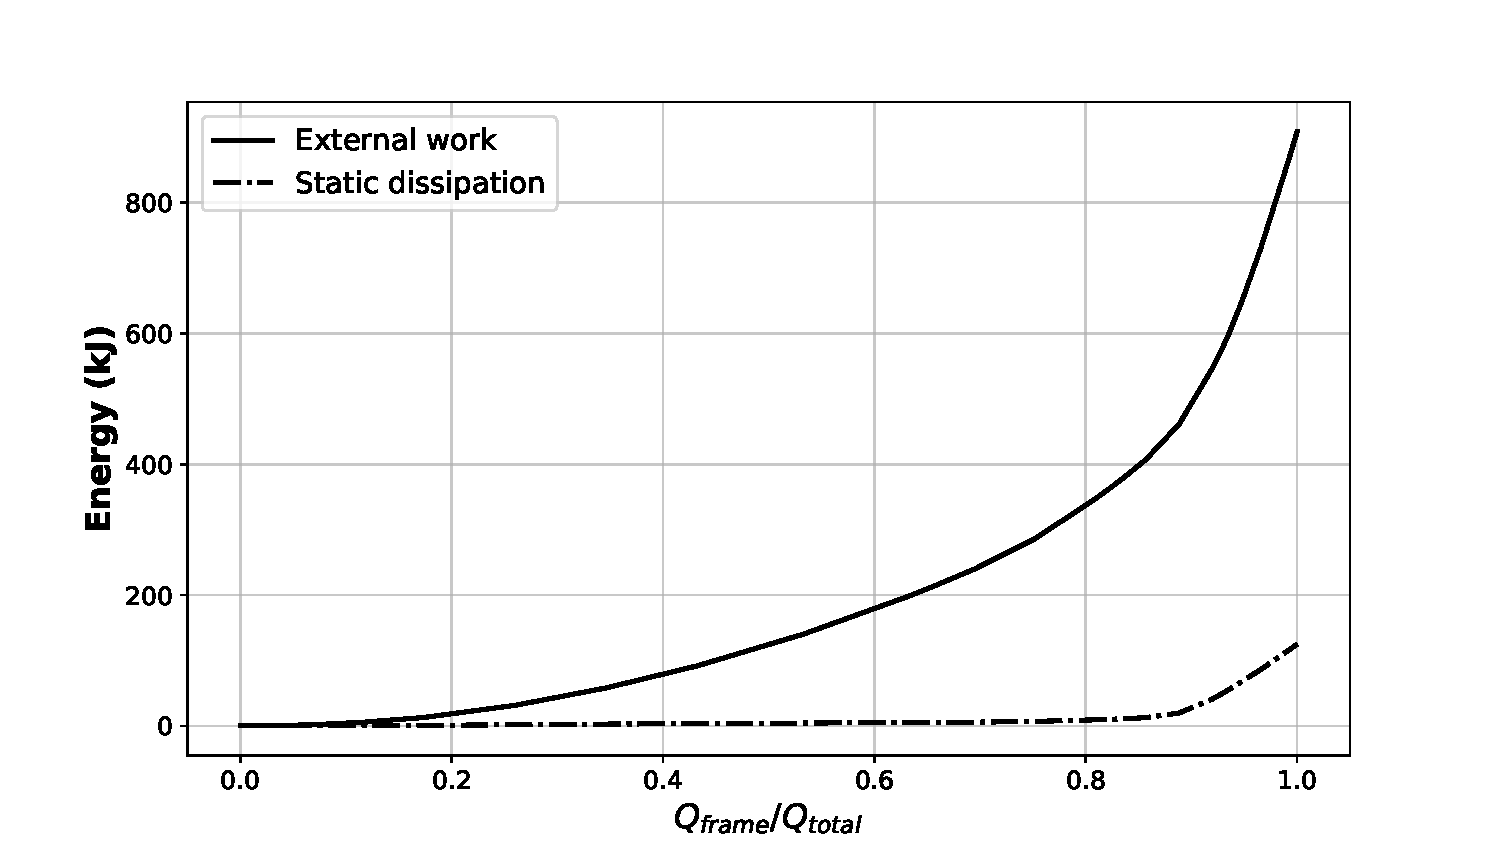
\includegraphics[width=0.8 \textwidth]{figures/result-model/energy_damp-5}
      \caption[External work and static dissipation for a damping factor equal to \notcien{2}{-5}]{External work and static dissipation for a damping factor equal to \notcien{2}{-5}. The positive slope of the curve showing the energy used in the static dissipation is a sign of over-damping.}\label{fig:energy_damp-5}
    \end{figure}

    \begin{figure}[!htpb]
      \centering
      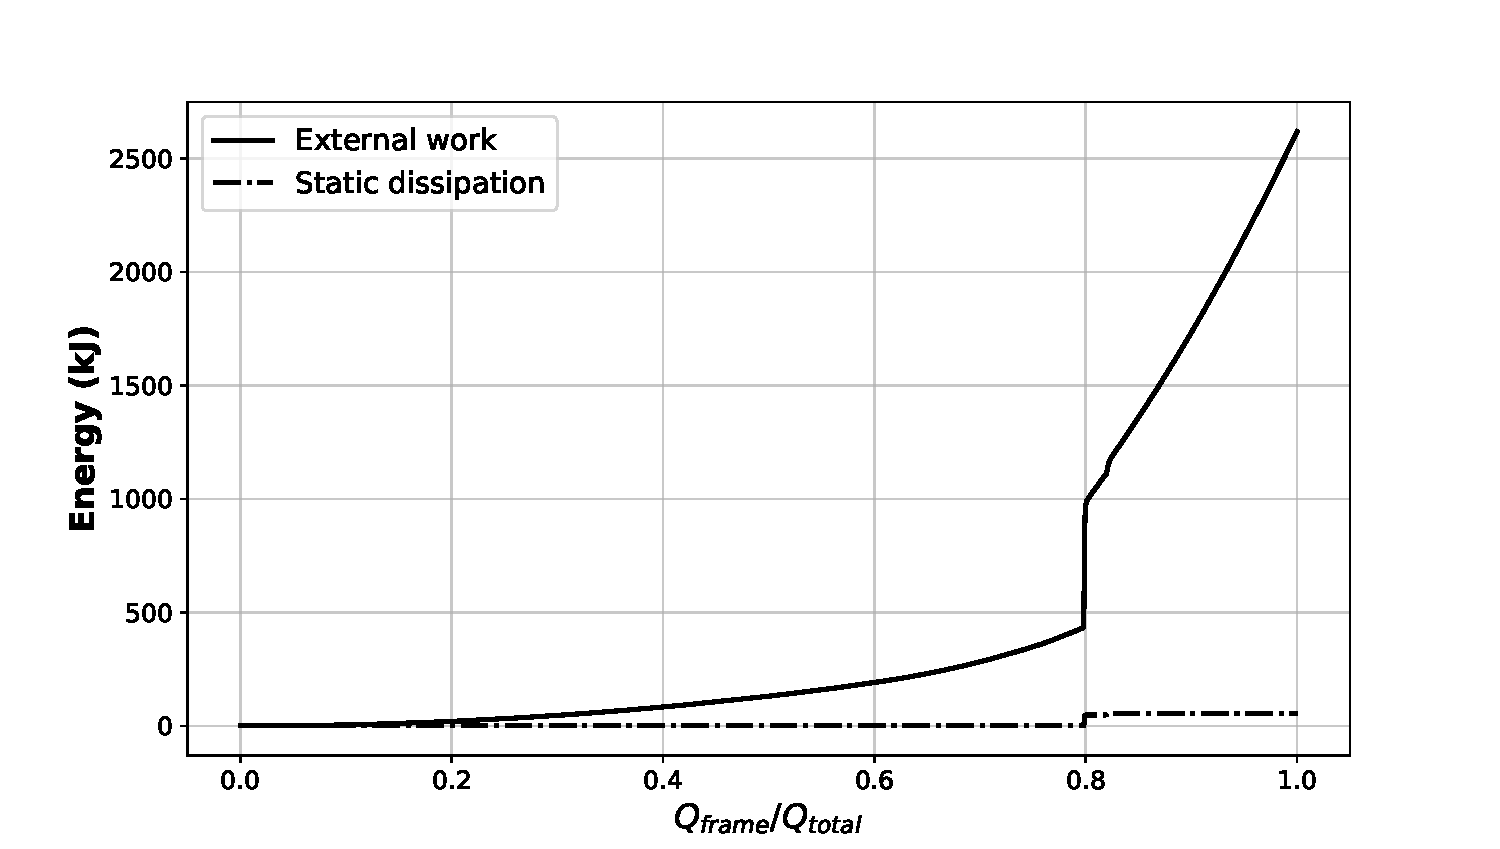
\includegraphics[width=0.8 \textwidth]{figures/result-model/energy_damp-8}
      \caption[External work and static dissipation for a damping factor equal to \notcien{2}{-8}]{External work and static dissipation for a damping factor equal to \notcien{2}{-8}. After the structure collapse the static dissipation energy remains constant and small compared with the external work introduced into the system.}\label{fig:energy_damp-8}
    \end{figure}

    \begin{figure}[!htpb]
      \centering
      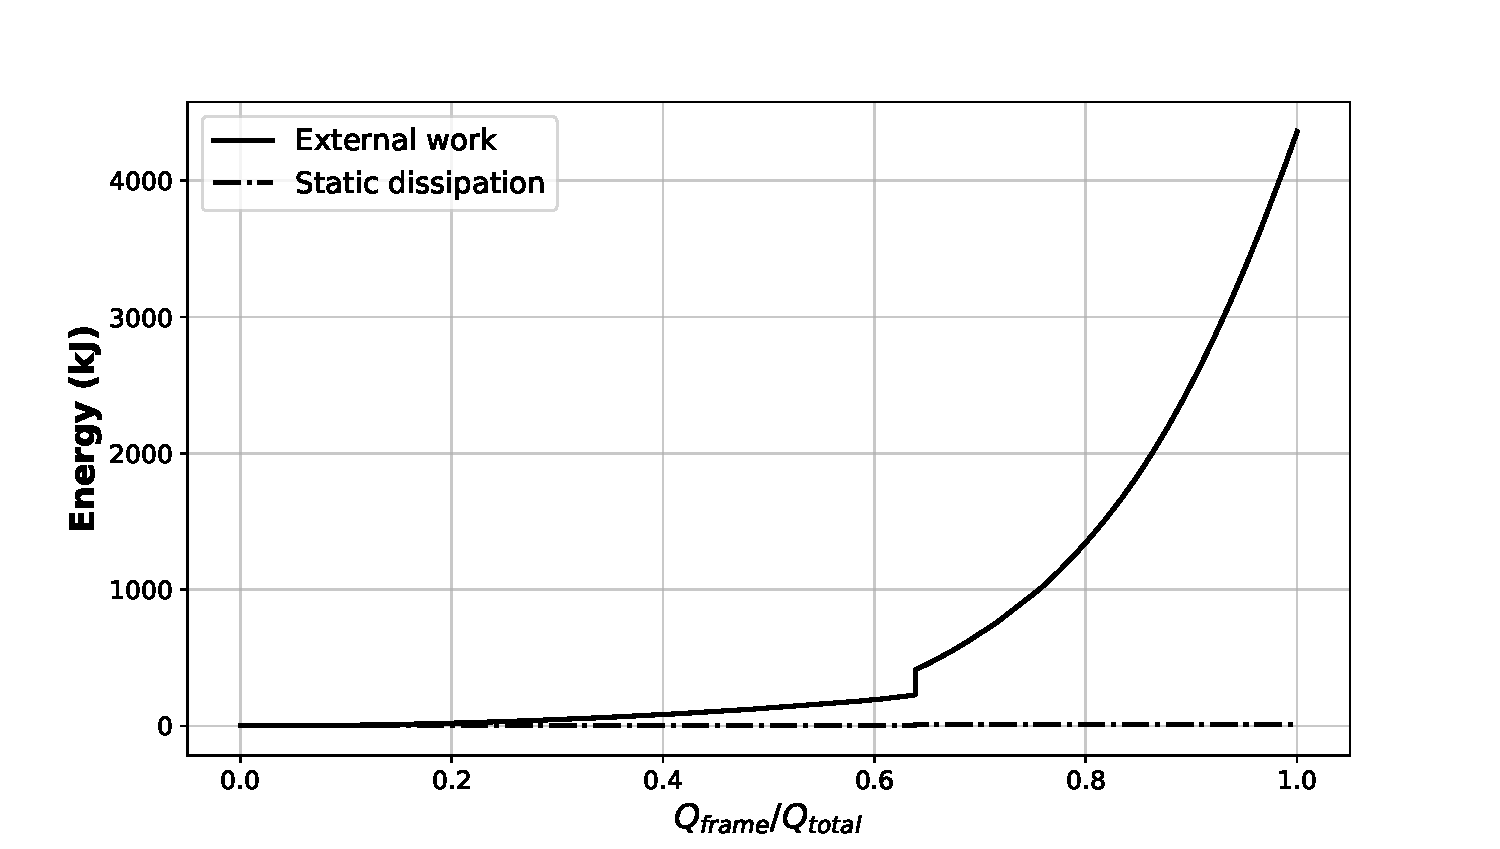
\includegraphics[width=0.8 \textwidth]{figures/result-model/energy_damp-9}
      \caption[External work and static dissipation for a damping factor equal to \notcien{2}{-9}]{External work and static dissipation for a damping factor equal to \notcien{2}{-9}. After the structure collapse the static dissipation energy remains constant and negligible compared with the external work introduced into the system.}\label{fig:energy_damp-9}
    \end{figure}

    Finally, since the objective is to capture the dynamics that involve buckling on the chiral ligaments and the ultimate collapse of the structure, keeping the energy dissipated a small as possible fraction of the external work, it is decided to use constant damping factor $c =$\notcien{2}{-9} for the simulations perform ahead. 

  \clearpage
  \subsection{Ribs inclusion and control over the local deformation} \label{subsec:ribs_results_model}
    %
    %Solution characterization
    % -> For the normal case
    %     - \ref{fig:normalCaseNoDampNoInnerRibs_800N}
    %     - the initial buckling ocurrs far from the root
    %     - UR1 of ~0.3 deg at the beam tip
    %
    % -> Introduccing damping
    %     - \ref{fig:normalCaseNoDampNoInnerRibs_800N}
    %     - Really big local deformations appear on the wing-box upper surface
    %     - UR1 of one order of magnitude higher, 3deg at the tip
    %     - Introduccing inner ribs becomes necessary to achieve greater twist with reduced local deformation
    %     - There is a point at which the structure collapses
    %     - \ref{fig:normalCaseDampNoInnerRibs}
    %     - See plot that compares the external work introduced in the system and the static energy dissipated through artificial stabilization. \ref{fig:normalCaseNoDampNoInnerRibs_800N_stabilizationPlot}
    %
    % -> Introducing inner ribs but not damping
    %     - \ref{fig:normalCaseNoDamp2InnerRibs_800N}
    %     - Buckling again appears at the front at it is very little
    %     - The simulation stops really soon, only tau/T = 0.134 achieved for the current plot
    % -> Introducing damping and inner ribs
    %     - Twist at the tip is now of about 0.68deg
    %     - The energy plot for this is \ref{fig:normalCaseDamp2InnerRibs_800N_stabilizationPLot}
    %     - The deformation plot shows now how buclking start at the lattice located close to the inner rib more close to the root, in a positive x from the position of the rib. The buckling then moves a group of lattices at the root, in the upper position of the lattice.
    %     - Some local deformation still ocurrs at the section of the wing-box skin located in between the root at the first inner rib.
    %     - However, the inner ribs help the upper skin of the wing-box to remain more flat than before.

    %First approach: no ribs, no damp
    As explained in Subsection \ref{subsubsec:Ribs_Parametrization}, two different designs are developed for the rib, one consists in a open profile and the other one in a closed profile. A first set of simulations are executed for the option of one open section at the rib at the tip. In Figure \ref{fig:closeOfRib-800N}, it can be seen an example of the response seen for this type of configuration after a prescribed load of 800 N has been applied. It can be seen that, under the prescribed load, the rib closes its profile and the upper flange shows a bigger displacement $v$ compared with the lower flange.

    \begin{figure}[!htpb]
      \centering
      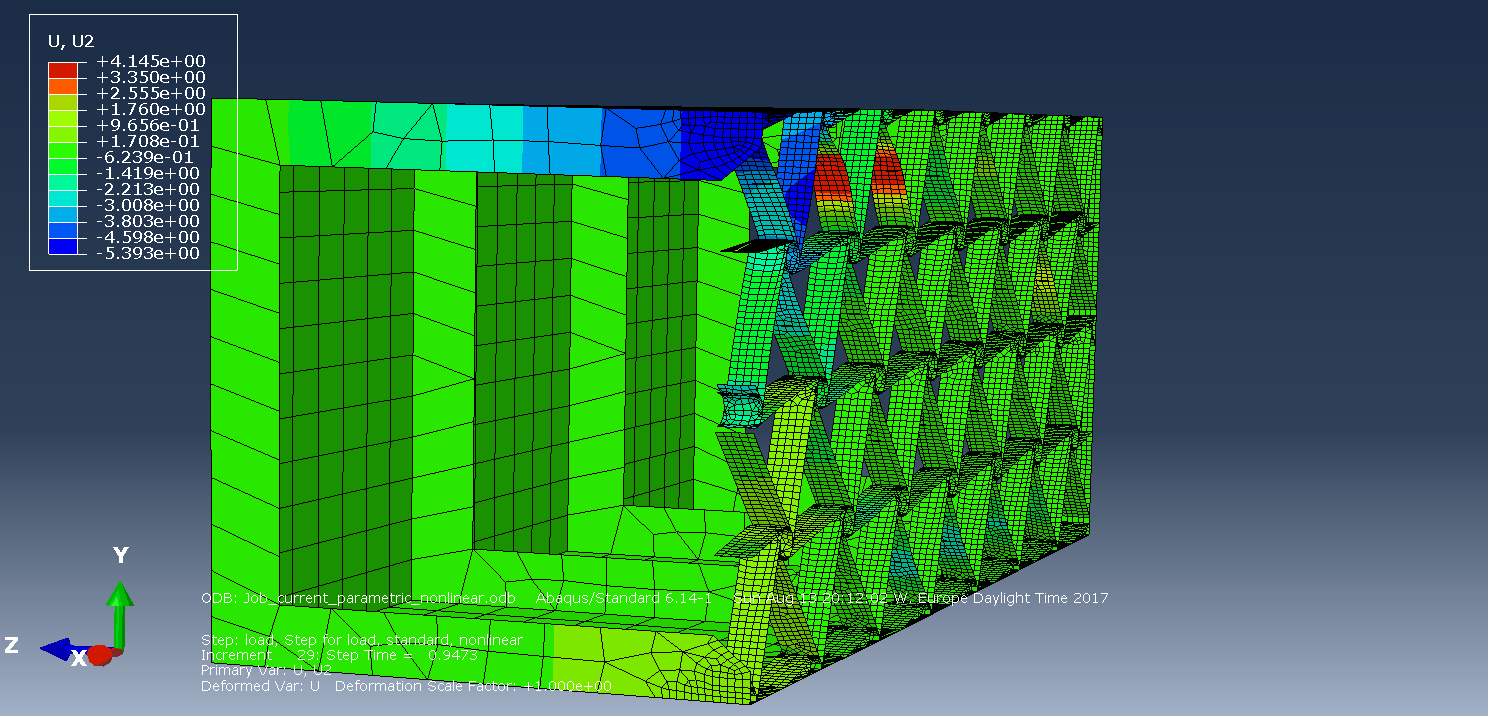
\includegraphics[width=0.8 \textwidth]{figures/result-model/closeOfRib-800N}
      \caption[Vertical displacement $v$ at the tip rib]{Vertical displacement $v$ at the tip rib. The colour contour shows those mesh nodes located on the upper flange of the rib have a higher $v$, therefore showing how the rib is closing under the prescribed load (800 N)}\label{fig:closeOfRib-800N}
    \end{figure}

    In an attempt to avoid a deformation in the rib that causes the rib to close, it was decided to use ribs with a close profile. Simulation are initially executed without incorporating automatic stabilization. Then, the colour contour plot of the total rotational displacement over the solution model is shown in Figure \ref{fig:normalCaseNoDampNoInnerRibs_800N}, where it can be seen that the initial buckling occurs in ligaments located far from the root. The twist of the beam, measured as the rotational displacement $u$ around the $x$ direction, is approximately 0.3 deg. The prescribed load as -800 N and the simulation converged to the 95\% of the prescribed load.

    \begin{figure}[!htpb]
      \centering
      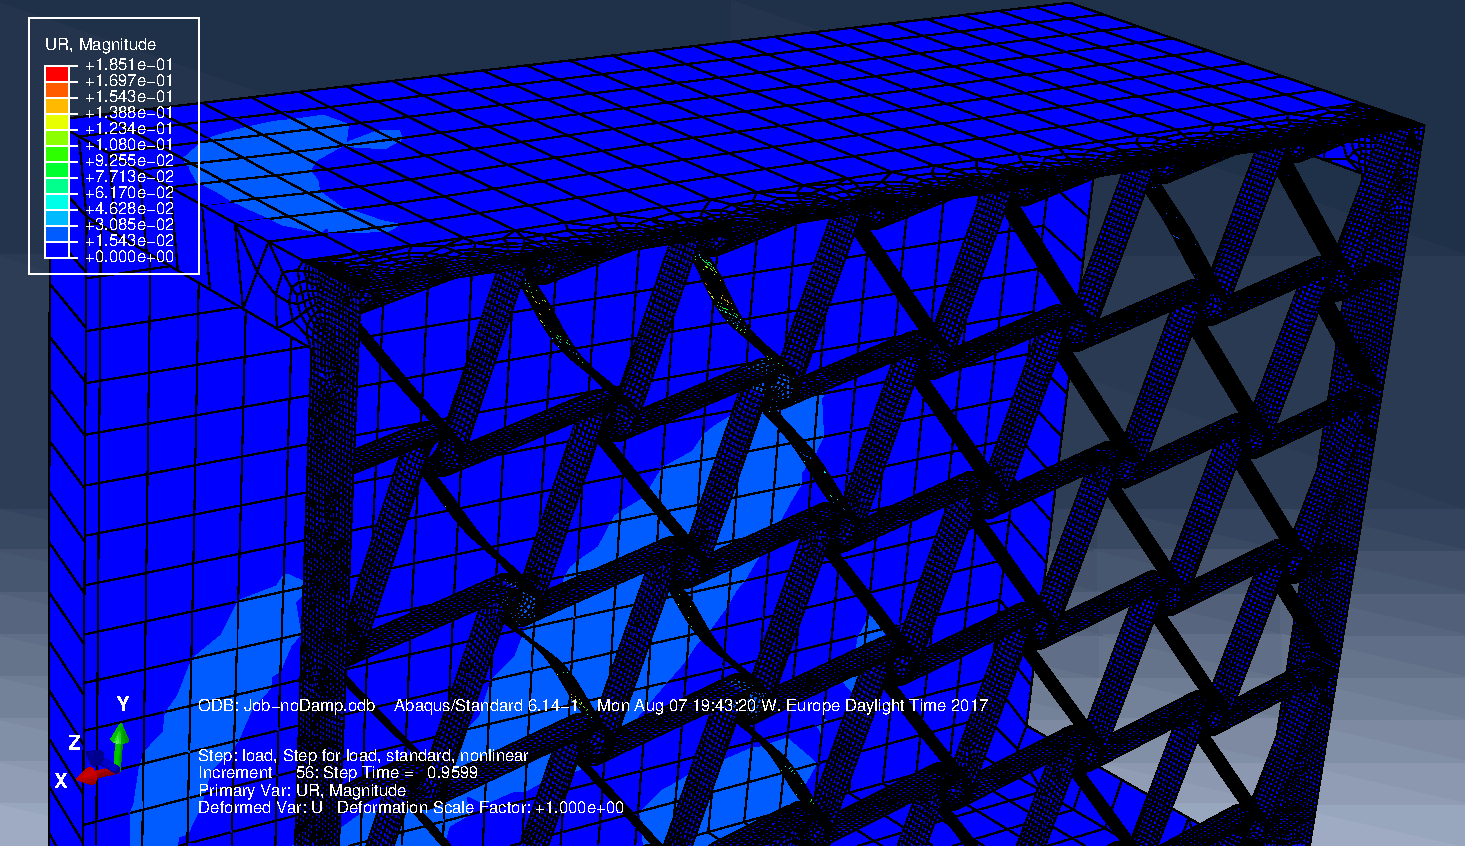
\includegraphics[width=0.8 \textwidth]{figures/result-model/normalCaseNoDampNoInnerRibs_800N}
      \caption[Model response without the use of inner ribs nor automatic stabilization]{Model response without the use of inner ribs nor automatic stabilization. The simulation converged to the 95\% of the prescribed load (800 N). Elastic deformations in the ligaments occur at the tip of the wing-box, close to the point where the load is introduced.}\label{fig:normalCaseNoDampNoInnerRibs_800N}
    \end{figure}

    In order to investigate further stages of the simulation, the addition of automatic stabilization through artificial damping factor becomes necessary, as it was explained in Subsection \ref{subsec:nonlinear_results_model}. After doing so, the colour contour plot of the total rotational displacement over the solution model is shown in Figure \ref{fig:normalCaseDampNoInnerRibs}. Apart from the buckling occurring at the chiral ligaments, this figure shows how big local deformations appear on the wing-box upper skin for this case. Also, it can be seen that the buckling phenomena has moved backwards to the ligaments close to the root.

    \begin{figure}[!htpb]
      \centering
      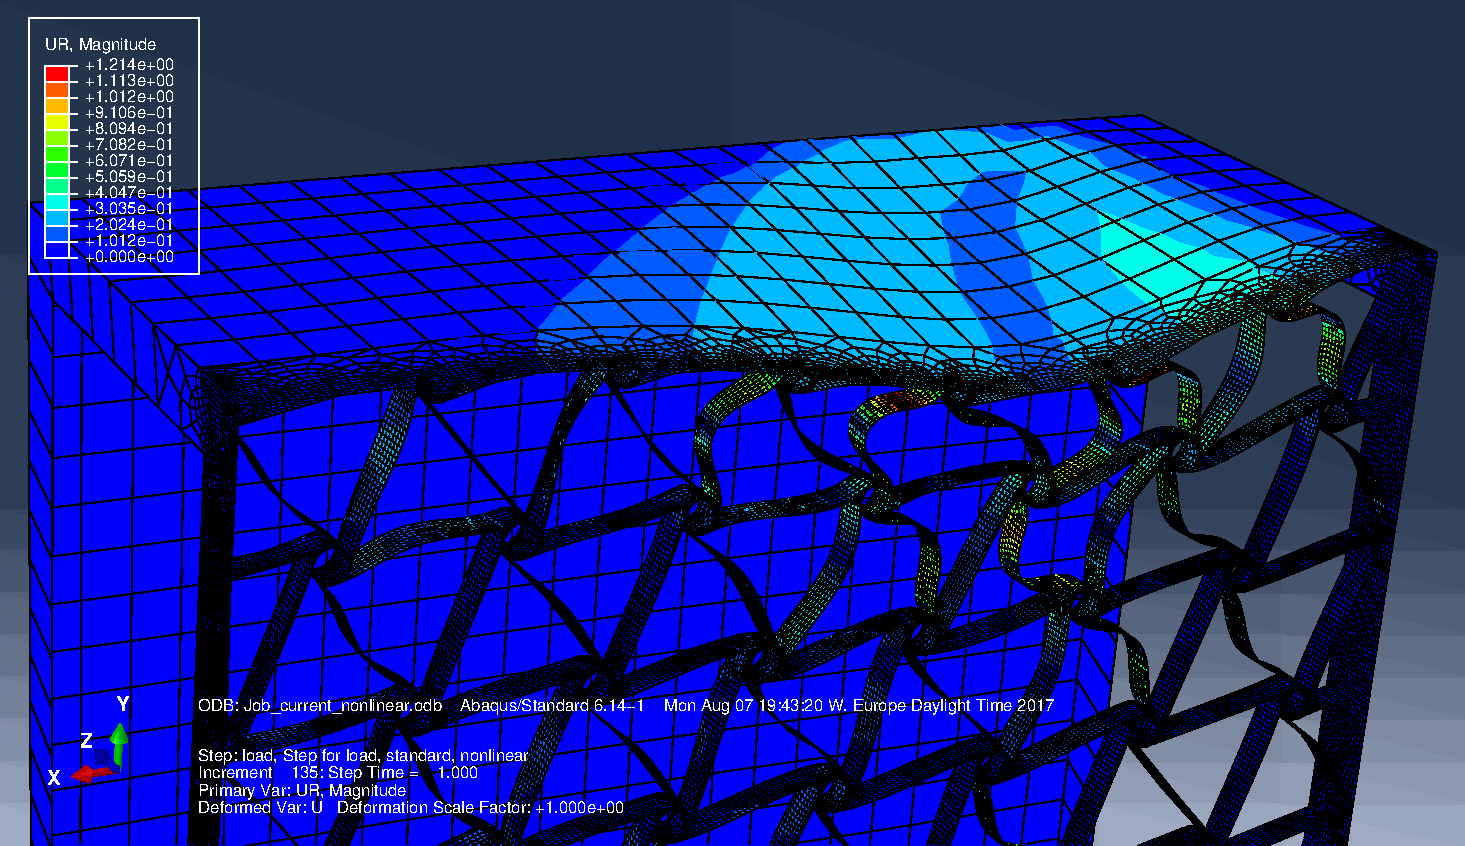
\includegraphics[width=0.8 \textwidth]{figures/result-model/normalCaseDampNoInnerRibs}
      \caption[Model response without the use of inner ribs and with automatic stabilization]{Model response without the use of inner ribs and with automatic stabilization. The simulation converged to the 100\% of the prescribed load (800 N). The inclusion of artificial constant damping factor allows the simulation to achieve further load increments, overpassing the point at which the collapse of the structure occurs. For the considered configuration and under the prescribed load, severe local deformations occurs at the wing-box skin which is needed to be accounted for.}\label{fig:normalCaseDampNoInnerRibs}
    \end{figure}

    %Inner ribs, no damp
    In order to reduce the local deformations occurring at the wing-box skin, a pair of inner ribs as described in Subsection \ref{subsec:parametrization_Model} are added to the model. This element adds stiffness to the structure in bending. Now, the colour contour with the total rotational displacement is shown in Figure \ref{fig:normalCaseNoDamp2InnerRibs}. Here it can be seen that the ligaments that start to buckle are located at the same position that they were when the model did not incorporate inner ribs. However, now the magnitude of local deformation at the wing-box skin has decreased due to the stiffness added to the structure as a result of the inner ribs inclusion.

    \begin{figure}[!htpb]
      \centering
      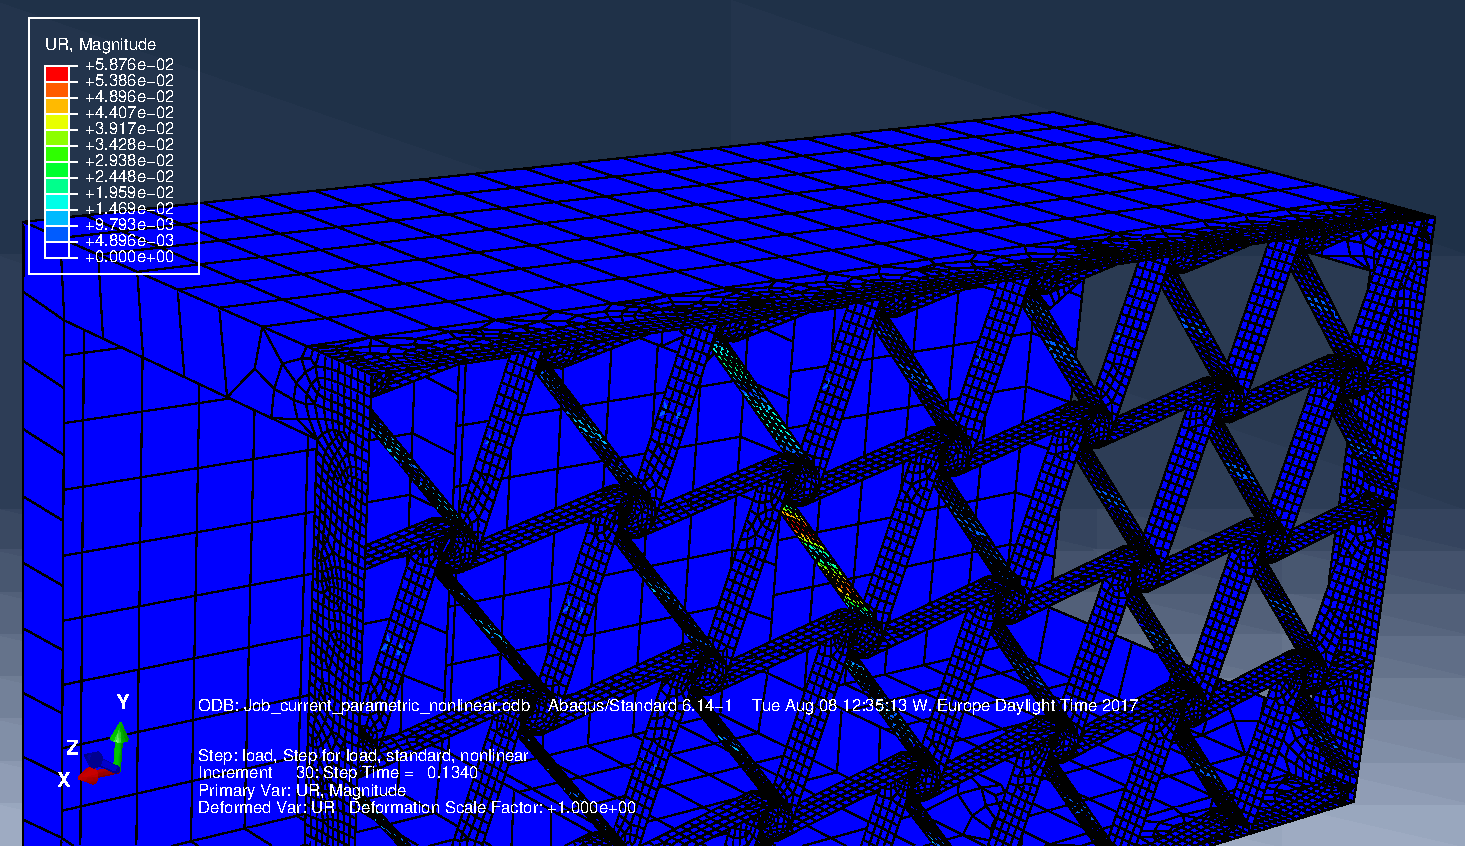
\includegraphics[width=0.8 \textwidth]{figures/result-model/normalCaseNoDamp2InnerRibs_800N}
      \caption[Model response incorporating inner ribs and without automatic stabilization]{Model response incorporating inner ribs and without automatic stabilization. The simulation converged to the 13\% of the prescribed load (800 N). The inner ribs have added stiffness to the structure in the bending.}
      \label{fig:normalCaseNoDamp2InnerRibs}
    \end{figure}

    %Now damp and inner ribs
    However, for this last case, the simulation was only able to converge up to 13\% of the prescribed load. In other to progress further in the analysis, the use of automatic stabilization becomes necessary again. For this reason, in the final configuration, automatic stabilization through constant damping factor is used together with the inner ribs. A description of the response of the structure for this last case is presented in next chapter.